% Options for packages loaded elsewhere
\PassOptionsToPackage{unicode}{hyperref}
\PassOptionsToPackage{hyphens}{url}
\PassOptionsToPackage{dvipsnames,svgnames,x11names}{xcolor}
%
\documentclass[
  letterpaper,
  DIV=11,
  numbers=noendperiod]{scrreprt}

\usepackage{amsmath,amssymb}
\usepackage{iftex}
\ifPDFTeX
  \usepackage[T1]{fontenc}
  \usepackage[utf8]{inputenc}
  \usepackage{textcomp} % provide euro and other symbols
\else % if luatex or xetex
  \usepackage{unicode-math}
  \defaultfontfeatures{Scale=MatchLowercase}
  \defaultfontfeatures[\rmfamily]{Ligatures=TeX,Scale=1}
\fi
\usepackage{lmodern}
\ifPDFTeX\else  
    % xetex/luatex font selection
\fi
% Use upquote if available, for straight quotes in verbatim environments
\IfFileExists{upquote.sty}{\usepackage{upquote}}{}
\IfFileExists{microtype.sty}{% use microtype if available
  \usepackage[]{microtype}
  \UseMicrotypeSet[protrusion]{basicmath} % disable protrusion for tt fonts
}{}
\makeatletter
\@ifundefined{KOMAClassName}{% if non-KOMA class
  \IfFileExists{parskip.sty}{%
    \usepackage{parskip}
  }{% else
    \setlength{\parindent}{0pt}
    \setlength{\parskip}{6pt plus 2pt minus 1pt}}
}{% if KOMA class
  \KOMAoptions{parskip=half}}
\makeatother
\usepackage{xcolor}
\usepackage{svg}
\setlength{\emergencystretch}{3em} % prevent overfull lines
\setcounter{secnumdepth}{5}
% Make \paragraph and \subparagraph free-standing
\makeatletter
\ifx\paragraph\undefined\else
  \let\oldparagraph\paragraph
  \renewcommand{\paragraph}{
    \@ifstar
      \xxxParagraphStar
      \xxxParagraphNoStar
  }
  \newcommand{\xxxParagraphStar}[1]{\oldparagraph*{#1}\mbox{}}
  \newcommand{\xxxParagraphNoStar}[1]{\oldparagraph{#1}\mbox{}}
\fi
\ifx\subparagraph\undefined\else
  \let\oldsubparagraph\subparagraph
  \renewcommand{\subparagraph}{
    \@ifstar
      \xxxSubParagraphStar
      \xxxSubParagraphNoStar
  }
  \newcommand{\xxxSubParagraphStar}[1]{\oldsubparagraph*{#1}\mbox{}}
  \newcommand{\xxxSubParagraphNoStar}[1]{\oldsubparagraph{#1}\mbox{}}
\fi
\makeatother

\usepackage{color}
\usepackage{fancyvrb}
\newcommand{\VerbBar}{|}
\newcommand{\VERB}{\Verb[commandchars=\\\{\}]}
\DefineVerbatimEnvironment{Highlighting}{Verbatim}{commandchars=\\\{\}}
% Add ',fontsize=\small' for more characters per line
\usepackage{framed}
\definecolor{shadecolor}{RGB}{241,243,245}
\newenvironment{Shaded}{\begin{snugshade}}{\end{snugshade}}
\newcommand{\AlertTok}[1]{\textcolor[rgb]{0.68,0.00,0.00}{#1}}
\newcommand{\AnnotationTok}[1]{\textcolor[rgb]{0.37,0.37,0.37}{#1}}
\newcommand{\AttributeTok}[1]{\textcolor[rgb]{0.40,0.45,0.13}{#1}}
\newcommand{\BaseNTok}[1]{\textcolor[rgb]{0.68,0.00,0.00}{#1}}
\newcommand{\BuiltInTok}[1]{\textcolor[rgb]{0.00,0.23,0.31}{#1}}
\newcommand{\CharTok}[1]{\textcolor[rgb]{0.13,0.47,0.30}{#1}}
\newcommand{\CommentTok}[1]{\textcolor[rgb]{0.37,0.37,0.37}{#1}}
\newcommand{\CommentVarTok}[1]{\textcolor[rgb]{0.37,0.37,0.37}{\textit{#1}}}
\newcommand{\ConstantTok}[1]{\textcolor[rgb]{0.56,0.35,0.01}{#1}}
\newcommand{\ControlFlowTok}[1]{\textcolor[rgb]{0.00,0.23,0.31}{\textbf{#1}}}
\newcommand{\DataTypeTok}[1]{\textcolor[rgb]{0.68,0.00,0.00}{#1}}
\newcommand{\DecValTok}[1]{\textcolor[rgb]{0.68,0.00,0.00}{#1}}
\newcommand{\DocumentationTok}[1]{\textcolor[rgb]{0.37,0.37,0.37}{\textit{#1}}}
\newcommand{\ErrorTok}[1]{\textcolor[rgb]{0.68,0.00,0.00}{#1}}
\newcommand{\ExtensionTok}[1]{\textcolor[rgb]{0.00,0.23,0.31}{#1}}
\newcommand{\FloatTok}[1]{\textcolor[rgb]{0.68,0.00,0.00}{#1}}
\newcommand{\FunctionTok}[1]{\textcolor[rgb]{0.28,0.35,0.67}{#1}}
\newcommand{\ImportTok}[1]{\textcolor[rgb]{0.00,0.46,0.62}{#1}}
\newcommand{\InformationTok}[1]{\textcolor[rgb]{0.37,0.37,0.37}{#1}}
\newcommand{\KeywordTok}[1]{\textcolor[rgb]{0.00,0.23,0.31}{\textbf{#1}}}
\newcommand{\NormalTok}[1]{\textcolor[rgb]{0.00,0.23,0.31}{#1}}
\newcommand{\OperatorTok}[1]{\textcolor[rgb]{0.37,0.37,0.37}{#1}}
\newcommand{\OtherTok}[1]{\textcolor[rgb]{0.00,0.23,0.31}{#1}}
\newcommand{\PreprocessorTok}[1]{\textcolor[rgb]{0.68,0.00,0.00}{#1}}
\newcommand{\RegionMarkerTok}[1]{\textcolor[rgb]{0.00,0.23,0.31}{#1}}
\newcommand{\SpecialCharTok}[1]{\textcolor[rgb]{0.37,0.37,0.37}{#1}}
\newcommand{\SpecialStringTok}[1]{\textcolor[rgb]{0.13,0.47,0.30}{#1}}
\newcommand{\StringTok}[1]{\textcolor[rgb]{0.13,0.47,0.30}{#1}}
\newcommand{\VariableTok}[1]{\textcolor[rgb]{0.07,0.07,0.07}{#1}}
\newcommand{\VerbatimStringTok}[1]{\textcolor[rgb]{0.13,0.47,0.30}{#1}}
\newcommand{\WarningTok}[1]{\textcolor[rgb]{0.37,0.37,0.37}{\textit{#1}}}

\providecommand{\tightlist}{%
  \setlength{\itemsep}{0pt}\setlength{\parskip}{0pt}}\usepackage{longtable,booktabs,array}
\usepackage{calc} % for calculating minipage widths
% Correct order of tables after \paragraph or \subparagraph
\usepackage{etoolbox}
\makeatletter
\patchcmd\longtable{\par}{\if@noskipsec\mbox{}\fi\par}{}{}
\makeatother
% Allow footnotes in longtable head/foot
\IfFileExists{footnotehyper.sty}{\usepackage{footnotehyper}}{\usepackage{footnote}}
\makesavenoteenv{longtable}
\usepackage{graphicx}
\makeatletter
\newsavebox\pandoc@box
\newcommand*\pandocbounded[1]{% scales image to fit in text height/width
  \sbox\pandoc@box{#1}%
  \Gscale@div\@tempa{\textheight}{\dimexpr\ht\pandoc@box+\dp\pandoc@box\relax}%
  \Gscale@div\@tempb{\linewidth}{\wd\pandoc@box}%
  \ifdim\@tempb\p@<\@tempa\p@\let\@tempa\@tempb\fi% select the smaller of both
  \ifdim\@tempa\p@<\p@\scalebox{\@tempa}{\usebox\pandoc@box}%
  \else\usebox{\pandoc@box}%
  \fi%
}
% Set default figure placement to htbp
\def\fps@figure{htbp}
\makeatother
% definitions for citeproc citations
\NewDocumentCommand\citeproctext{}{}
\NewDocumentCommand\citeproc{mm}{%
  \begingroup\def\citeproctext{#2}\cite{#1}\endgroup}
\makeatletter
 % allow citations to break across lines
 \let\@cite@ofmt\@firstofone
 % avoid brackets around text for \cite:
 \def\@biblabel#1{}
 \def\@cite#1#2{{#1\if@tempswa , #2\fi}}
\makeatother
\newlength{\cslhangindent}
\setlength{\cslhangindent}{1.5em}
\newlength{\csllabelwidth}
\setlength{\csllabelwidth}{3em}
\newenvironment{CSLReferences}[2] % #1 hanging-indent, #2 entry-spacing
 {\begin{list}{}{%
  \setlength{\itemindent}{0pt}
  \setlength{\leftmargin}{0pt}
  \setlength{\parsep}{0pt}
  % turn on hanging indent if param 1 is 1
  \ifodd #1
   \setlength{\leftmargin}{\cslhangindent}
   \setlength{\itemindent}{-1\cslhangindent}
  \fi
  % set entry spacing
  \setlength{\itemsep}{#2\baselineskip}}}
 {\end{list}}
\usepackage{calc}
\newcommand{\CSLBlock}[1]{\hfill\break\parbox[t]{\linewidth}{\strut\ignorespaces#1\strut}}
\newcommand{\CSLLeftMargin}[1]{\parbox[t]{\csllabelwidth}{\strut#1\strut}}
\newcommand{\CSLRightInline}[1]{\parbox[t]{\linewidth - \csllabelwidth}{\strut#1\strut}}
\newcommand{\CSLIndent}[1]{\hspace{\cslhangindent}#1}

\KOMAoption{captions}{tableheading}
\makeatletter
\@ifpackageloaded{tcolorbox}{}{\usepackage[skins,breakable]{tcolorbox}}
\@ifpackageloaded{fontawesome5}{}{\usepackage{fontawesome5}}
\definecolor{quarto-callout-color}{HTML}{909090}
\definecolor{quarto-callout-note-color}{HTML}{0758E5}
\definecolor{quarto-callout-important-color}{HTML}{CC1914}
\definecolor{quarto-callout-warning-color}{HTML}{EB9113}
\definecolor{quarto-callout-tip-color}{HTML}{00A047}
\definecolor{quarto-callout-caution-color}{HTML}{FC5300}
\definecolor{quarto-callout-color-frame}{HTML}{acacac}
\definecolor{quarto-callout-note-color-frame}{HTML}{4582ec}
\definecolor{quarto-callout-important-color-frame}{HTML}{d9534f}
\definecolor{quarto-callout-warning-color-frame}{HTML}{f0ad4e}
\definecolor{quarto-callout-tip-color-frame}{HTML}{02b875}
\definecolor{quarto-callout-caution-color-frame}{HTML}{fd7e14}
\makeatother
\makeatletter
\@ifpackageloaded{bookmark}{}{\usepackage{bookmark}}
\makeatother
\makeatletter
\@ifpackageloaded{caption}{}{\usepackage{caption}}
\AtBeginDocument{%
\ifdefined\contentsname
  \renewcommand*\contentsname{Table of contents}
\else
  \newcommand\contentsname{Table of contents}
\fi
\ifdefined\listfigurename
  \renewcommand*\listfigurename{List of Figures}
\else
  \newcommand\listfigurename{List of Figures}
\fi
\ifdefined\listtablename
  \renewcommand*\listtablename{List of Tables}
\else
  \newcommand\listtablename{List of Tables}
\fi
\ifdefined\figurename
  \renewcommand*\figurename{Figure}
\else
  \newcommand\figurename{Figure}
\fi
\ifdefined\tablename
  \renewcommand*\tablename{Table}
\else
  \newcommand\tablename{Table}
\fi
}
\@ifpackageloaded{float}{}{\usepackage{float}}
\floatstyle{ruled}
\@ifundefined{c@chapter}{\newfloat{codelisting}{h}{lop}}{\newfloat{codelisting}{h}{lop}[chapter]}
\floatname{codelisting}{Listing}
\newcommand*\listoflistings{\listof{codelisting}{List of Listings}}
\makeatother
\makeatletter
\makeatother
\makeatletter
\@ifpackageloaded{caption}{}{\usepackage{caption}}
\@ifpackageloaded{subcaption}{}{\usepackage{subcaption}}
\makeatother
\makeatletter
\@ifpackageloaded{algorithm}{}{\usepackage{algorithm}}
\makeatother
\makeatletter
\@ifpackageloaded{algpseudocode}{}{\usepackage{algpseudocode}}
\makeatother
\makeatletter
\@ifpackageloaded{caption}{}{\usepackage{caption}}
\makeatother

\usepackage{bookmark}

\IfFileExists{xurl.sty}{\usepackage{xurl}}{} % add URL line breaks if available
\urlstyle{same} % disable monospaced font for URLs
\hypersetup{
  pdftitle={DATS 6450 -- Reinforcement Learning},
  pdfauthor={Tyler Wallett, MS \& Amir Jafari, PhD},
  colorlinks=true,
  linkcolor={blue},
  filecolor={Maroon},
  citecolor={Blue},
  urlcolor={Blue},
  pdfcreator={LaTeX via pandoc}}


\title{DATS 6450 -- Reinforcement Learning}
\author{Tyler Wallett, MS \& Amir Jafari, PhD}
\date{2025-03-13}

\begin{document}
\maketitle

\floatname{algorithm}{Algorithm}

\numberwithin{algorithm}{chapter}

\renewcommand*\contentsname{Table of contents}
{
\hypersetup{linkcolor=}
\setcounter{tocdepth}{2}
\tableofcontents
}

\bookmarksetup{startatroot}

\chapter{DATS 6450 -- Reinforcement
Learning}\label{dats-6450-reinforcement-learning}

\section{Instructor Information}\label{instructor-information}

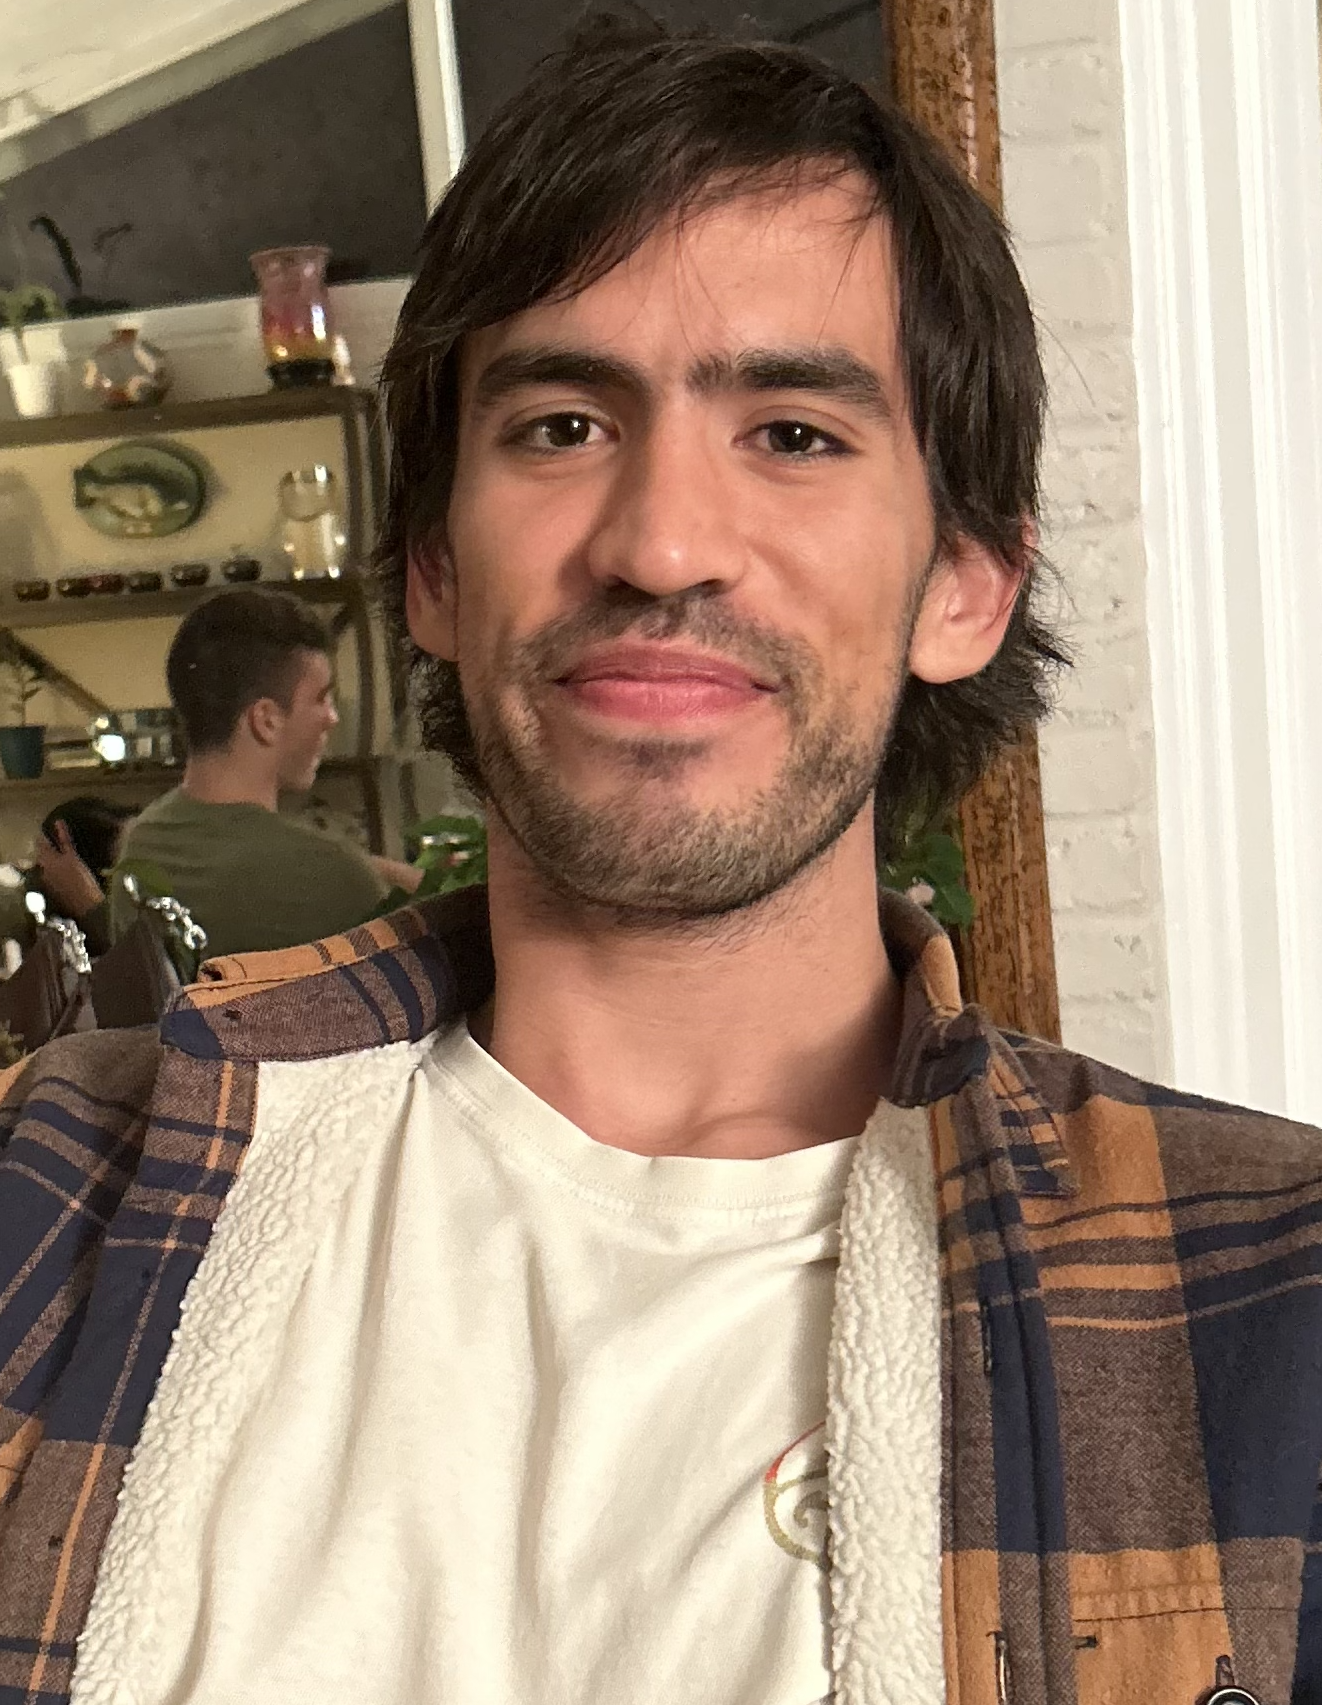
\includegraphics[width=2.08333in,height=2.60417in]{data/images/me.png}

\begin{itemize}
\tightlist
\item
  \textbf{Name:} Tyler Wallett, M.S.\\
\item
  \textbf{Term:} Fall 2025\\
\item
  \textbf{Office location:} Samson Hall Room 310\\
\item
  \textbf{Office hours:} TBD\\
\item
  \textbf{E-mail:}
  \href{mailto:twallett@gwu.edu}{\nolinkurl{twallett@gwu.edu}}\\
\item
  \textbf{Github:} \href{https://github.com/twallett}{twallett}\\
\item
  \textbf{Zoom:} Meeting Link\\
\end{itemize}

\section{Course Description}\label{course-description}

The aim of this course is to provide a comprehensive understanding of
the \textbf{reinforcement learning framework}. The course will explore
the key distinctions between reinforcement learning and other artificial
intelligence learning paradigms, delve into relevant industry
applications, and examine both classical and deep learning approaches.
Additionally, the course will cover the taxonomy of reinforcement
learning and offer hands-on experience through practical implementations
using OpenAI Gymnasium and other learning environments.

The \textbf{classical approach} will focus on learning methods designed
to find optimal solutions in tabular environments, whereas the
\textbf{deep learning approach} will tackle the challenge of finding
approximate optimal solutions in large or continuous environments
through the use of deep learning architectures.

The course will introduce the \textbf{taxonomy of reinforcement
learning} by focusing on model-free value-based methods, transitioning
to value function approximation and deep learning approaches, followed
by novel policy-based methods using state-of-the-art architectures to
tackle complex environments.

To conclude, a discussion on \textbf{advanced topics, applications, and
outlook} of reinforcement learning will be provided.

\section{Learning Outcomes}\label{learning-outcomes}

\begin{enumerate}
\def\labelenumi{\arabic{enumi}.}
\tightlist
\item
  Implement Reinforcement Learning frameworks using \texttt{numpy} and
  \texttt{tensorflow}.
\item
  Design decision-making systems using classical and deep learning
  architectures.
\item
  Explain the Reinforcement Learning taxonomy.
\item
  Identify Reinforcement Learning's challenges, current research, and
  future outlook.
\end{enumerate}

\section{Resources}\label{resources}

\begin{itemize}
\tightlist
\item
  \emph{Reinforcement Learning: An Introduction} by Richard S. Sutton
  and Andrew G. Barto
  (\href{https://www.andrew.cmu.edu/course/10-703/textbook/BartoSutton.pdf}{Web
  Link})
\end{itemize}

\section{Software Requirements}\label{software-requirements}

\begin{itemize}
\tightlist
\item
  \textbf{Programming:} Python.
\end{itemize}

\begin{Shaded}
\begin{Highlighting}[]
\ExtensionTok{pip}\NormalTok{ install numpy}
\ExtensionTok{pip}\NormalTok{ install tensorflow}
\ExtensionTok{pip}\NormalTok{ install pygame}
\ExtensionTok{pip}\NormalTok{ install gymnasium}
\ExtensionTok{pip}\NormalTok{ install stable{-}baselines3}
\end{Highlighting}
\end{Shaded}

\begin{itemize}
\tightlist
\item
  \textbf{Cloud Services:} Google Colab.
\end{itemize}

\section{Course Outline}\label{course-outline}

\begin{longtable}[]{@{}
  >{\raggedright\arraybackslash}p{(\linewidth - 6\tabcolsep) * \real{0.1353}}
  >{\raggedright\arraybackslash}p{(\linewidth - 6\tabcolsep) * \real{0.3308}}
  >{\raggedright\arraybackslash}p{(\linewidth - 6\tabcolsep) * \real{0.1278}}
  >{\raggedright\arraybackslash}p{(\linewidth - 6\tabcolsep) * \real{0.4060}}@{}}
\toprule\noalign{}
\begin{minipage}[b]{\linewidth}\raggedright
Week
\end{minipage} & \begin{minipage}[b]{\linewidth}\raggedright
Topic
\end{minipage} & \begin{minipage}[b]{\linewidth}\raggedright
Quiz/Exams
\end{minipage} & \begin{minipage}[b]{\linewidth}\raggedright
Subjects
\end{minipage} \\
\midrule\noalign{}
\endhead
\bottomrule\noalign{}
\endlastfoot
Aug 29, 2025 & Introduction to Reinforcement Learning & & - Course
Outline - Why should I study Reinforcement Learning? - What is
Reinforcement Learning? - Where is Reinforcement Learning Applied? - How
is Reinforcement Learning Structured?  \\
Sep 5, 2025 & Mathematical Foundations & & - Set Theory - Axiomatic
Probability - Conditioning - Independence - Random Variables -
Expectation - Probability Distribution \\
Sep 12, 2025 & Multi-Armed Bandits & Quiz 1 & - Multi-Armed Bandit
Framework - \(\epsilon\)-Greedy - Upper Confidence Boundary (UCB) -
Thompson Sampling \\
Sep 19, 2025 & Dynamic Programming & Quiz 2 & - Markov Chain - Markov
Decision Process (MDPs) - Dynamic Programming \\
Sep 26, 2025 & Monte Carlo & Quiz 3 & - OpenAI Gymansium Environment:
GridWorld - Monte Carlo Prediction - Exploring Starts Monte Carlo -
On-Policy Monte Carlo - Off-Policy Monte Carlo \\
Oct 3, 2025 & Temporal Difference & Quiz 4 & - OpenAI Gymansium
Environment: GridWorld - Temporal Difference (TD) Prediction - SARSA -
Q-Learning - Double Q-Learning - (Optional) n-step TD \\
Oct 10, 2025 & Function Approximation & \textbf{Exam 1} & - OpenAI
Gymansium Environment: MountainCar - Value Function Approximation (VFA)
- On-Policy Function Approximation - Semi-gradient SARSA - Limitations
of Off-Policy Function Approximation \\
Oct 24, 2025 & Deep Q-Networks & Quiz 5 & - OpenAI Gymansium
Environment: BreakOut - Multi-Layered Perceprtons (MLPs) - Convolutional
Neural Networks (CNNs) - Experience Replay - Fixed Targets - Vanilla
Deep Q-Network \\
Oct 31, 2025 & Policy Gradients & Quiz 6 & - OpenAI Gymansium
Environment: CartPole - Policy Gradient Theorem - Vanilla Policy
Gradient \\
Nov 7, 2025 & Advanced Policy Gradients & Quiz 7 & - OpenAI Gymansium
Environment: HalfCheetah - Trust Region Policy Optimization (TRPO) -
Proximal Policy Optimization: KL-Divergence - Proximal Policy
Optimization: Clip \\
Nov 14, 2025 & \textbf{Thanksgiving Break} & & \\
Nov 21, 2025 & Monte Carlo Tree Search & \textbf{Exam 2} & - OpenAI
Gymansium Environment: Tic Tac Toe - Model-based Reinforcement Learning
- Monte Carlo Tree Search - AlphaGo - MuZero \\
Oct 28, 2025 & Conclusion & & \\
Dec 5, 2025 & Final Project Submission & & \\
\end{longtable}

\section{Prerequisites}\label{prerequisites}

\begin{itemize}
\tightlist
\item
  \textbf{DATS 6101} - Introduction to Data Science
\end{itemize}

\section{Assignments \& Grading}\label{assignments-grading}

\begin{longtable}[]{@{}cc@{}}
\toprule\noalign{}
Assignment & Points \\
\midrule\noalign{}
\endhead
\bottomrule\noalign{}
\endlastfoot
Quizzes (5 best scores) & 25 \\
Exam 1 & 25 \\
Exam 2 & 25 \\
Final Project & 25 \\
\end{longtable}

\begin{tcolorbox}[enhanced jigsaw, opacityback=0, left=2mm, breakable, bottomtitle=1mm, rightrule=.15mm, colframe=quarto-callout-note-color-frame, titlerule=0mm, colback=white, opacitybacktitle=0.6, toptitle=1mm, title=\textcolor{quarto-callout-note-color}{\faInfo}\hspace{0.5em}{Average Learning Per Week}, colbacktitle=quarto-callout-note-color!10!white, bottomrule=.15mm, arc=.35mm, coltitle=black, leftrule=.75mm, toprule=.15mm]

Students are expected to spend a minimum of 100 minutes of out-of-class
work for every 50 minutes of direct instruction, for a minimum total of
2.5 hours a week. A 3-credit course should include 2.5 hours of direct
instruction and a minimum of 5 hours of independent learning or 7.5
hours per week.

\end{tcolorbox}

\begin{tcolorbox}[enhanced jigsaw, opacityback=0, left=2mm, breakable, bottomtitle=1mm, rightrule=.15mm, colframe=quarto-callout-note-color-frame, titlerule=0mm, colback=white, opacitybacktitle=0.6, toptitle=1mm, title=\textcolor{quarto-callout-note-color}{\faInfo}\hspace{0.5em}{Online Resources}, colbacktitle=quarto-callout-note-color!10!white, bottomrule=.15mm, arc=.35mm, coltitle=black, leftrule=.75mm, toprule=.15mm]

For technical requirements and support, student services, obtaining a
GWorld card, and state contact information please check
\href{online.gwu.edu/student-support}{HERE}

\end{tcolorbox}

\begin{tcolorbox}[enhanced jigsaw, opacityback=0, left=2mm, breakable, bottomtitle=1mm, rightrule=.15mm, colframe=quarto-callout-note-color-frame, titlerule=0mm, colback=white, opacitybacktitle=0.6, toptitle=1mm, title=\textcolor{quarto-callout-note-color}{\faInfo}\hspace{0.5em}{Classroom Recording}, colbacktitle=quarto-callout-note-color!10!white, bottomrule=.15mm, arc=.35mm, coltitle=black, leftrule=.75mm, toprule=.15mm]

The particular class recordings will be available to students who are
registered on an individual basis, upon request. Please let me know in
advance if you have any medical issues or emergencies that will prevent
you from joining the class.

\end{tcolorbox}

\begin{tcolorbox}[enhanced jigsaw, opacityback=0, left=2mm, breakable, bottomtitle=1mm, rightrule=.15mm, colframe=quarto-callout-tip-color-frame, titlerule=0mm, colback=white, opacitybacktitle=0.6, toptitle=1mm, title=\textcolor{quarto-callout-tip-color}{\faLightbulb}\hspace{0.5em}{Virtual Academic Support}, colbacktitle=quarto-callout-tip-color!10!white, bottomrule=.15mm, arc=.35mm, coltitle=black, leftrule=.75mm, toprule=.15mm]

A full range of academic support is offered virtually in fall 2020. See
\href{coronavirus.gwu.edu/top-faqs}{HERE} for updates. Tutoring and
course review sessions are offered through Academic Commons in an online
format. See \href{academiccommons.gwu.edu/tutoring}{HERE}. Writing and
research consultations are available online. See
\href{academiccommons.gwu.edu/writing-research-help}{HERE}. Coaching,
offered through the Office of Student Success, is available in a virtual
format. See
\href{studentsuccess.gwu.edu/academic-program-support}{HERE}. Academic
Commons offers several short videos addressing different virtual
learning strategies for the unique circumstances of the fall 2020
semester. See \href{academiccommons.gwu.edu/study-skills}{HERE}. They
also offer a variety of live virtual workshops to equip students with
the tools they need to succeed in a virtual environment. See
\href{tinyurl.com/gw-virtual-learning}{HERE}.

\end{tcolorbox}

\begin{tcolorbox}[enhanced jigsaw, opacityback=0, left=2mm, breakable, bottomtitle=1mm, rightrule=.15mm, colframe=quarto-callout-warning-color-frame, titlerule=0mm, colback=white, opacitybacktitle=0.6, toptitle=1mm, title=\textcolor{quarto-callout-warning-color}{\faExclamationTriangle}\hspace{0.5em}{Safety and Security}, colbacktitle=quarto-callout-warning-color!10!white, bottomrule=.15mm, arc=.35mm, coltitle=black, leftrule=.75mm, toprule=.15mm]

In an emergency: call GWPD 202-994-6111 or 911. For situation-specific
actions: review the Emergency Response Handbook in
\href{safety.gwu.edu/emergency-response-handbook}{HERE}. In an active
violence situation: Get Out, Hide Out, or Take Out. See
\href{go.gwu.edu/shooterpret}{HERE}. Stay informed:
safety.gwu.edu/stay-informed.

\end{tcolorbox}

\part{Lecture 1: Introduction}

\chapter{1.1 Why should I study Reinforcement
Learning?}\label{why-should-i-study-reinforcement-learning}

\begin{tcolorbox}[enhanced jigsaw, colback=white, left=2mm, breakable, opacityback=0, bottomrule=.15mm, rightrule=.15mm, arc=.35mm, colframe=quarto-callout-note-color-frame, leftrule=.75mm, toprule=.15mm]

Welcome to DATS 6450: Reinforcement Learning! 🚀 Before diving into
algorithms and mathematical calculations we must first stop and ask
ourselves the essential question:

Why should I study Reinforcement Learning? 🤔

\end{tcolorbox}

\section{Advances in Artificial
Intelligence}\label{advances-in-artificial-intelligence}

\begin{itemize}
\item
  \textbf{June 2018}: OpenAI introduces the Generative Pre-trained
  Transformer (GPT), laying the foundation for subsequent LLMs.
\item
  \textbf{February 2019}: OpenAI releases GPT-2, demonstrating
  significant improvements in text generation capabilities.
\item
  \textbf{June 2020}: GPT-3 is unveiled, featuring 175 billion
  parameters and showcasing advanced language understanding and
  generation.
\item
  \textbf{January 2021}: OpenAI announces DALL-E, a model capable of
  generating images from textual descriptions.
\item
  \textbf{April 2022}: DALL-E 2 is introduced, offering enhanced image
  resolution and greater realism in generated images.
\item
  \textbf{November 2022}: OpenAI releases ChatGPT, a conversational AI
  based on the GPT-3.5 architecture, enabling more interactive and
  contextually relevant dialogues.
\end{itemize}

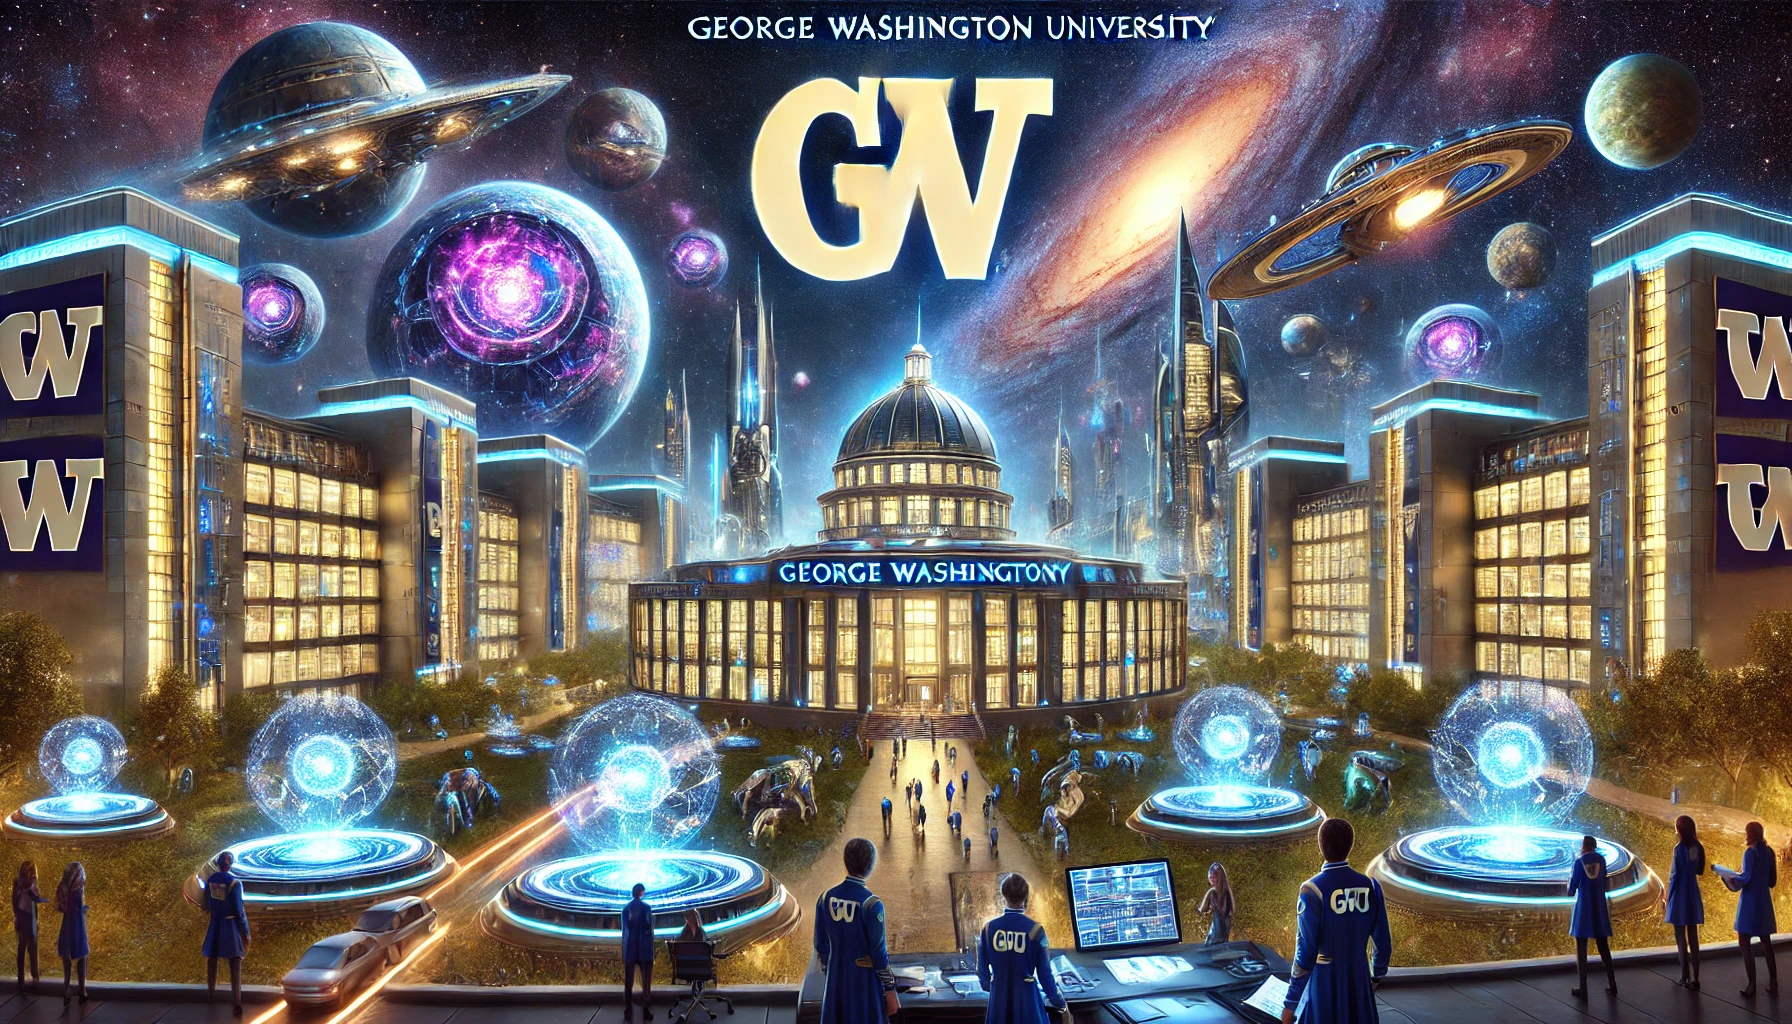
\includegraphics[width=1\linewidth,height=3.125in]{lecture1/images/diffusion.png}


\includegraphics[width=1\linewidth,height=3.125in]{lecture1/images/diffusion2.png}

At GWU, where minds aspire, Reinforcement learners never tire In search
of policies, bold and bright, They train their agents, day and night.
With Sutton, Barto as their guide, They walk the path, rewards beside.
Exploring states with epsilon's grace, They find the optimal embrace.
Gridworlds vast, mazes deep, In code they sow, in dreams they reap. The
future's theirs, they push, they strive-- GWU's learners, alive, alive!

Poem and images generated by \textbf{Large Language Model: ChatGPT 3.5}
\& \textbf{Diffusion Models: DALL-E}, correspondingly.

In essence, the AI model's behavior closely mirrors human-like actions.
This is expected, given its training on extensive datasets derived from
human behavior. However, continued training on the same datasets will
likely result in models that perform at a human-equivalent level. To
achieve significant breakthroughs, we must explore learning methods that
transcend typical human capabilities.

\section{The Goal of Reinforcement
Learning}\label{the-goal-of-reinforcement-learning}

\begin{tcolorbox}[enhanced jigsaw, opacityback=0, left=2mm, breakable, bottomtitle=1mm, rightrule=.15mm, colframe=quarto-callout-tip-color-frame, titlerule=0mm, colback=white, opacitybacktitle=0.6, toptitle=1mm, title=\textcolor{quarto-callout-tip-color}{\faLightbulb}\hspace{0.5em}{Emergent Behavior}, colbacktitle=quarto-callout-tip-color!10!white, bottomrule=.15mm, arc=.35mm, coltitle=black, leftrule=.75mm, toprule=.15mm]

Reinforcement Learning is concerned with seeking \emph{emergent
behavior}, or behavior that goes beyond what people might do or think
of.

\end{tcolorbox}

Ultimately, as scientists, we want to discover new solutions for a task
so that when an agent, or decision-maker, is placed in a novel situation
it can respond intelligently (Levine 2019).

\subsection{Example: AlphaGO}\label{example-alphago}

\begin{figure}[H]

{\centering \pandocbounded{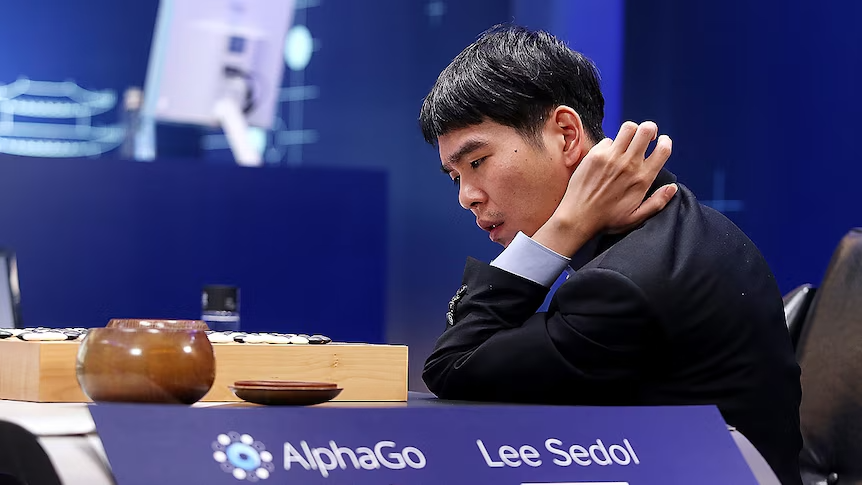
\includegraphics[keepaspectratio]{lecture1/images/go.png}}

}

\caption{AlphaGo Move 37}

\end{figure}%

``\emph{It's not a human move. I've never seen a human play this
move.}'' -- Commentator on Move 37, AlphaGo (2017)

\subsection{Example: Matrix
Multiplication}\label{example-matrix-multiplication}

\begin{figure}[H]

{\centering \pandocbounded{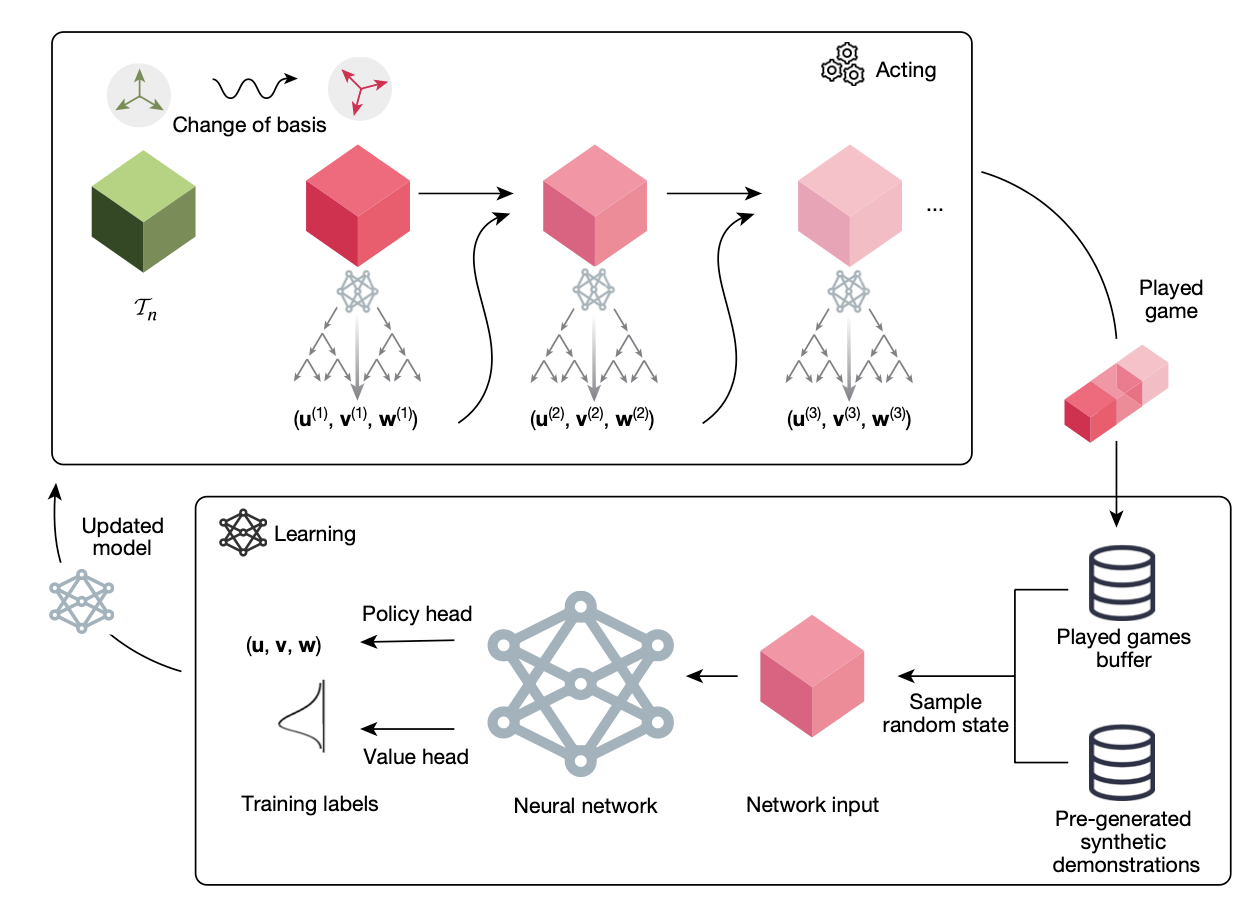
\includegraphics[keepaspectratio]{lecture1/images/MatrixMultiplication.png}}

}

\caption{Discovering faster matrix multiplication algorithms with
reinforcement learning}

\end{figure}%

``\emph{Trained from scratch, AlphaTensor discovers matrix
multiplication algorithms that are more efficient than existing human
and computer-designed algorithms.}'' - Discovering faster matrix
multiplication algorithms with reinforcement learning

\section{So why should I study Reinforcement
Learning?}\label{so-why-should-i-study-reinforcement-learning}

Reinforcement Learning (RL) is not just another machine learning
paradigm; it is a fundamental framework for decision-making, control,
and optimizing sequential actions in uncertain environments. Studying RL
enables us to:

✅ Understand Intelligence ✅ Develop Cutting-Edge AI ✅ Solve
Real-World Problems ✅ Push Beyond Human Limits

By studying RL, we gain the tools to create AI that learns, adapts, and
innovates beyond predefined rules and static datasets. 🚀

\chapter{1.2 What is Reinforcement
Learning?}\label{what-is-reinforcement-learning}

\begin{tcolorbox}[enhanced jigsaw, colback=white, left=2mm, breakable, opacityback=0, bottomrule=.15mm, rightrule=.15mm, arc=.35mm, colframe=quarto-callout-note-color-frame, leftrule=.75mm, toprule=.15mm]

So now that we have answered the fundamental question of why. It's time
for the next big mystery:

What is Reinforcement Learning? 🤔

\end{tcolorbox}

Good news! We can sum up the core idea of Reinforcement Learning in just
one powerful sentence (Brunskill 2022):

\chapter{Learning Optimal Sequential Decision-Making Under
Uncertainty}\label{learning-optimal-sequential-decision-making-under-uncertainty}

But what exactly does that mean? Let's break it down!

\section{Learning}\label{learning}

At its core, learning in Reinforcement Learning occurs through trial and
error, where an agent refines its actions based on \emph{evaluative
feedback} from the environment.

\begin{tcolorbox}[enhanced jigsaw, opacityback=0, left=2mm, breakable, bottomtitle=1mm, rightrule=.15mm, colframe=quarto-callout-tip-color-frame, titlerule=0mm, colback=white, opacitybacktitle=0.6, toptitle=1mm, title=\textcolor{quarto-callout-tip-color}{\faLightbulb}\hspace{0.5em}{Evaluative Feedback}, colbacktitle=quarto-callout-tip-color!10!white, bottomrule=.15mm, arc=.35mm, coltitle=black, leftrule=.75mm, toprule=.15mm]

\emph{Evaluative feedback} indicates how good the action taken was, but
not whether it was the best or the worst action.

Intuition: Learning through experience

\end{tcolorbox}

\begin{figure}[H]

{\centering 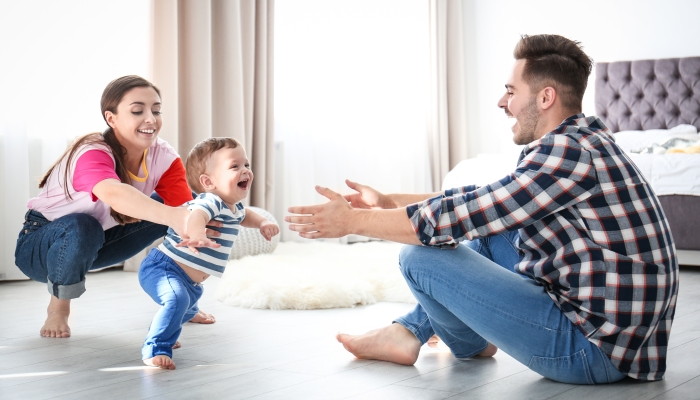
\includegraphics[width=1\linewidth,height=2.08333in]{lecture1/images/BabyWalking.jpg}

}

\caption{Learning to Walk}

\end{figure}%

\begin{figure}[H]

{\centering 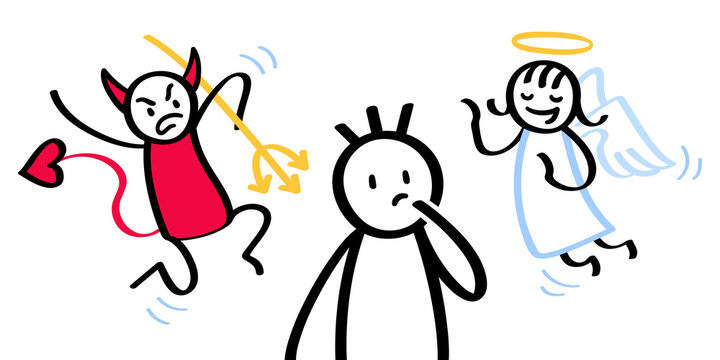
\includegraphics[width=1\linewidth,height=2.08333in]{lecture1/images/ethics.jpg}

}

\caption{Ethics (Right vs.~Wrong)}

\end{figure}%

Unlike both supervised/unsupervised learning which rely on
\emph{instructive feedback} through gradient based optimization.

\begin{tcolorbox}[enhanced jigsaw, opacityback=0, left=2mm, breakable, bottomtitle=1mm, rightrule=.15mm, colframe=quarto-callout-tip-color-frame, titlerule=0mm, colback=white, opacitybacktitle=0.6, toptitle=1mm, title=\textcolor{quarto-callout-tip-color}{\faLightbulb}\hspace{0.5em}{Instructive Feedback}, colbacktitle=quarto-callout-tip-color!10!white, bottomrule=.15mm, arc=.35mm, coltitle=black, leftrule=.75mm, toprule=.15mm]

\emph{Instructive feedback} indicates the correct action to take,
independently of the action actually taken.

Intuition: Learning through ground truth

\end{tcolorbox}

\begin{figure}[H]

{\centering 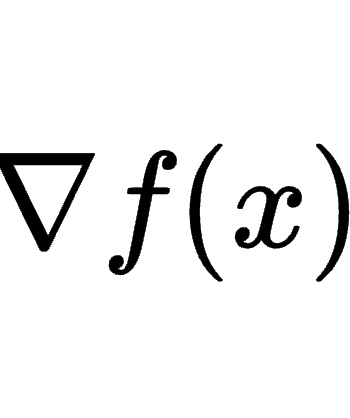
\includegraphics[width=0.25\linewidth,height=2.08333in]{lecture1/images/nabla.drawio.png}

}

\caption{Supervised/Unsupervised Learning}

\end{figure}%

For example, supervised/unsupervised learning focus on identifying what
makes an image a cheetah by learning patterns from a dataset of animal
images. In contrast, Reinforcement Learning is about teaching a cheetah
how to run by interacting with its environment (Lecture 10).

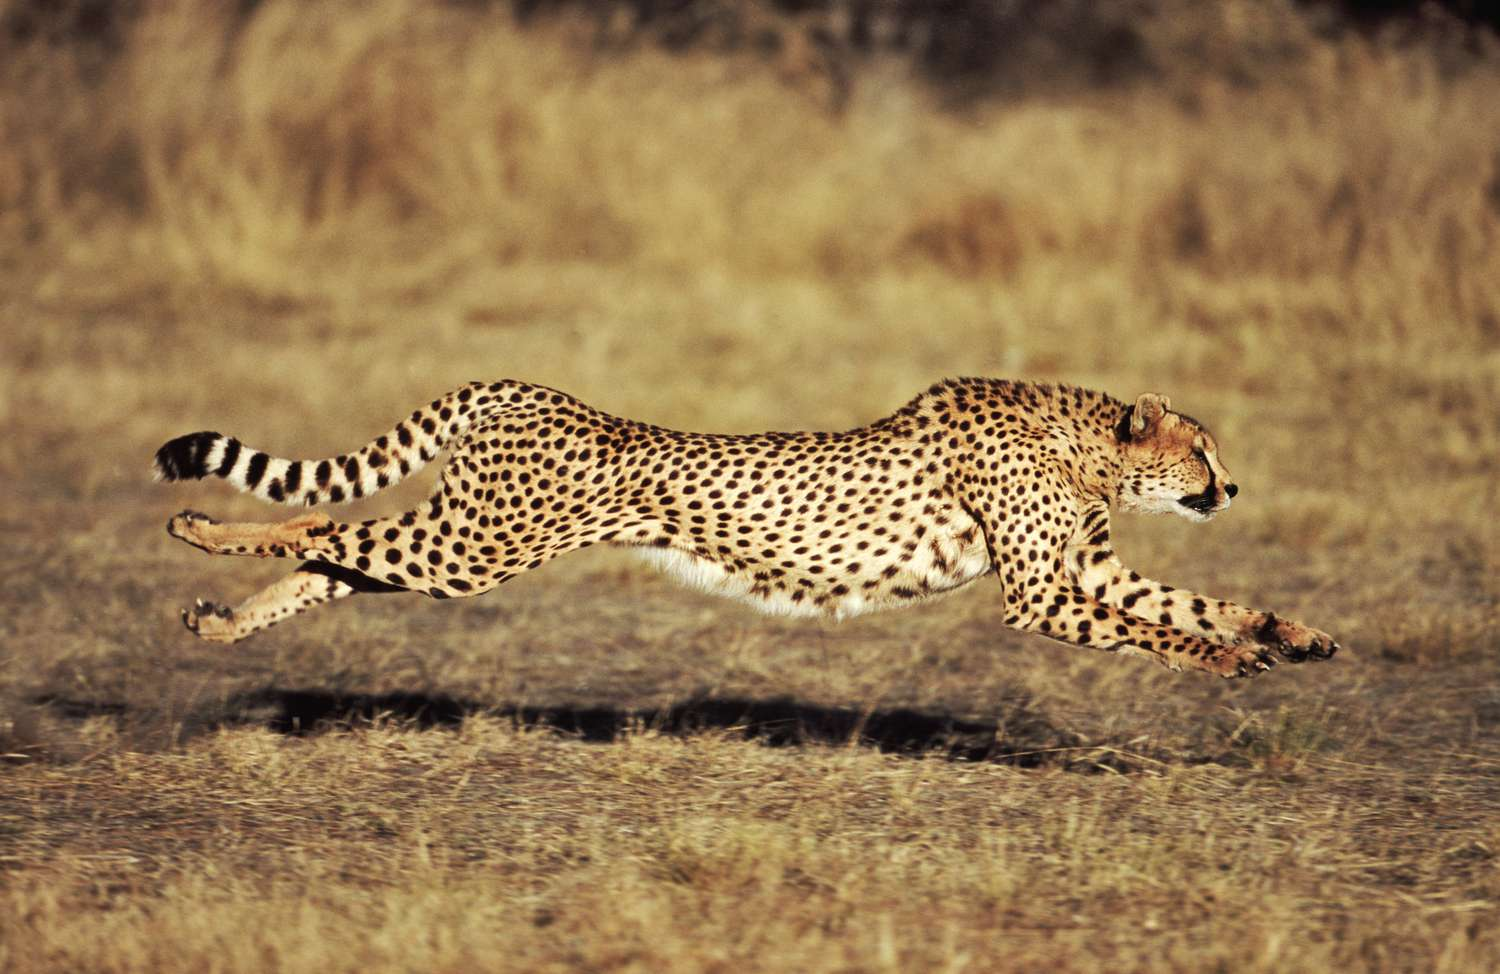
\includegraphics[width=1\linewidth,height=2.08333in]{lecture1/images/cheetah.jpg}
``Here's some examples (images), now learn patterns in these
examples\ldots{}''

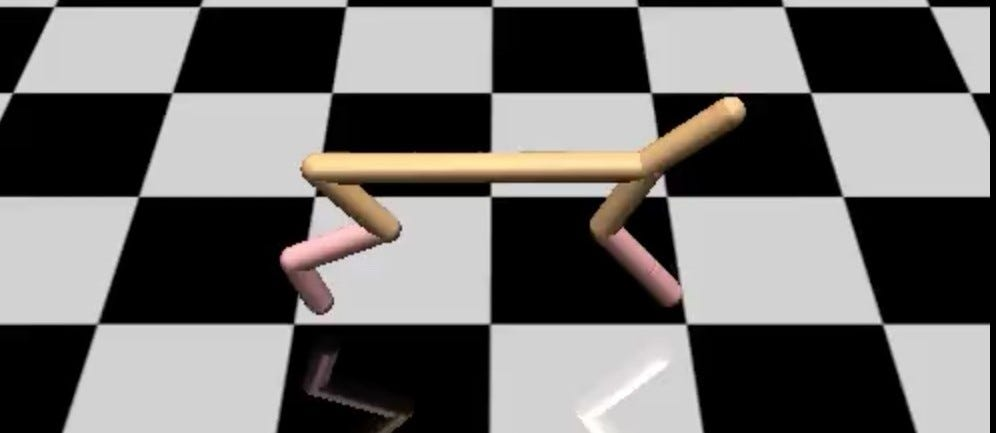
\includegraphics[width=1\linewidth,height=2.08333in]{lecture1/images/cheetahopenai.jpg}
``Here's an environment, now learn patterns by exploring it\ldots{}''

\section{Optimal}\label{optimal}

The goal of Reinforcement Learning is to maximize rewards over time by
finding the best possible strategy. This involves seeking:

\begin{itemize}
\tightlist
\item
  A Maximized discounted sum of rewards, or goal \(G\).
\item
  Optimal Value Functions \(V^{*}\).
\item
  Optimal Action-Value Functions \(Q^{*}\).
\item
  Optimal Policies \(\pi^{*}\).
\item
  A Balance between exploration vs.~exploitation.
\end{itemize}

\section{Sequential Decision-Making}\label{sequential-decision-making}

Unlike a one-time choice, Reinforcement Learning involves a chain of
decisions where each action affects the next.

\begin{figure}[H]

{\centering \pandocbounded{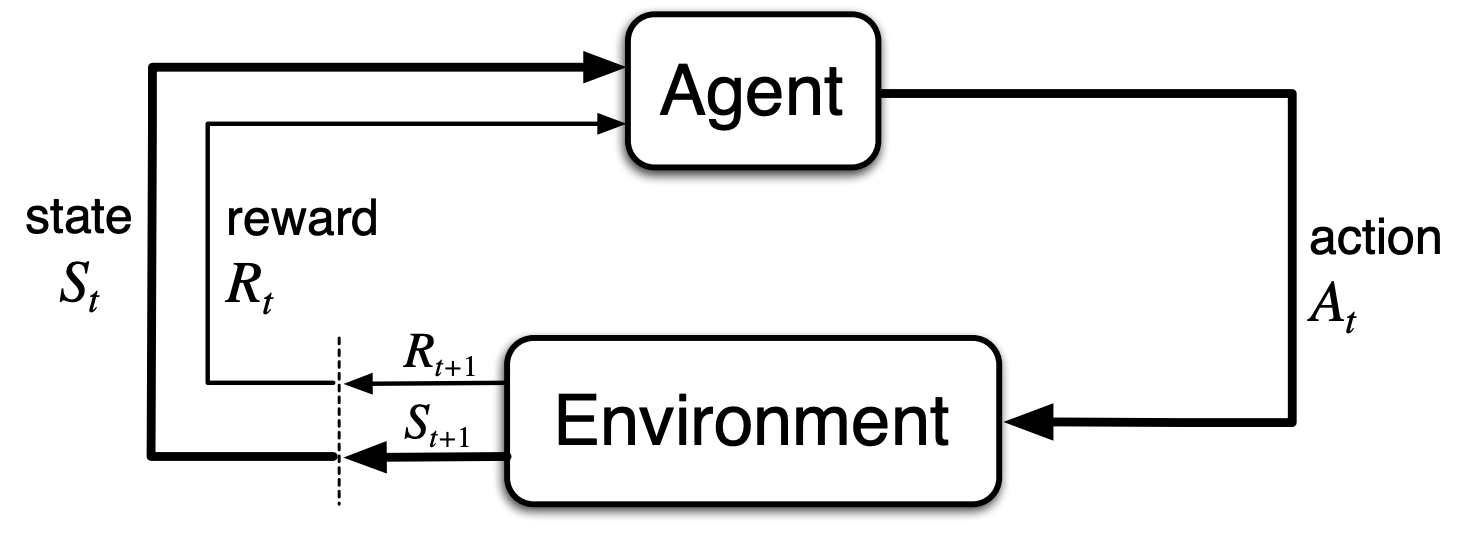
\includegraphics[keepaspectratio]{lecture1/images/MDP.png}}

}

\caption{Markov Decision Process}

\end{figure}%

\(\pi: S_{0}, A_{0}, R_{1}, S_{1}, A_{1}, R_{2}, ... , S_{T-1}, A_{T-1}, R_{T}\)

\begin{itemize}
\tightlist
\item
  Markov Decision Process (MDP) is a formal framework for modeling
  decision-making.
\item
  The agent selects actions over multiple time steps, shaping its future
  states and rewards.
\item
  Each decision affects not only immediate rewards but also the
  trajectory of future outcomes.
\end{itemize}

\chapter{1.3 Where is Reinforcement Learning
Applied?}\label{where-is-reinforcement-learning-applied}

\begin{tcolorbox}[enhanced jigsaw, colback=white, left=2mm, breakable, opacityback=0, bottomrule=.15mm, rightrule=.15mm, arc=.35mm, colframe=quarto-callout-note-color-frame, leftrule=.75mm, toprule=.15mm]

We know why it matters and what it's all about. Now, let's dive into:

Where is Reinforcement Learning Applied? 🤔

\end{tcolorbox}

\section{Recommendation Systems}\label{recommendation-systems}

Reinforcement Learning powers modern recommendation systems by
dynamically adapting to user preferences, optimizing content suggestions
in platforms like Netflix, YouTube, and Spotify using techniques such as
Multi-Armed Bandits (MAB).

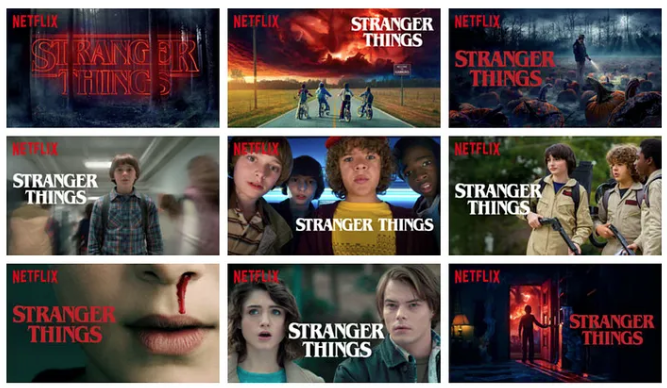
\includegraphics[width=0.5\linewidth,height=\textheight,keepaspectratio]{lecture1/images/Neflix.png}\\
Trained using MAB (Lecture 2)\\
\href{https://netflixtechblog.com/artwork-personalization-c589f074ad76}{Link
to Online Article}

\section{Games}\label{games}

Reinforcement Learning has revolutionized gaming by enabling AI to
master complex environments, from Atari classics to advanced strategy
games, using deep learning techniques like Deep Q-Networks (DQN) to
achieve superhuman performance.

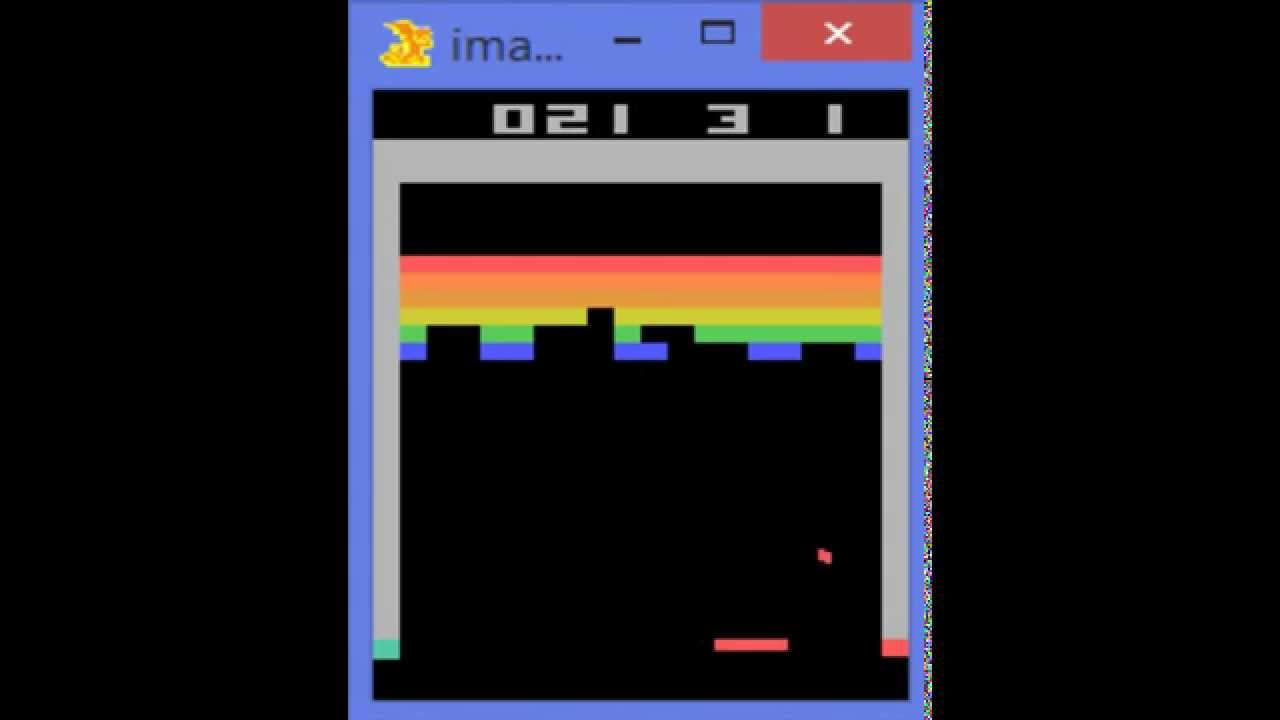
\includegraphics[width=\linewidth,height=0.7\textheight,keepaspectratio]{lecture1/images/breakout.gif}\\
Trained using DQN (Lecture 9)\\
\href{https://arxiv.org/pdf/1312.5602}{Link to Research Paper}

\section{Robotics}\label{robotics}

In robotics, Reinforcement Learning enables autonomous agents to learn
complex motor skills, such as dexterous manipulation and locomotion,
through continuous interaction and training with Proximal Policy
Optimization (PPO).

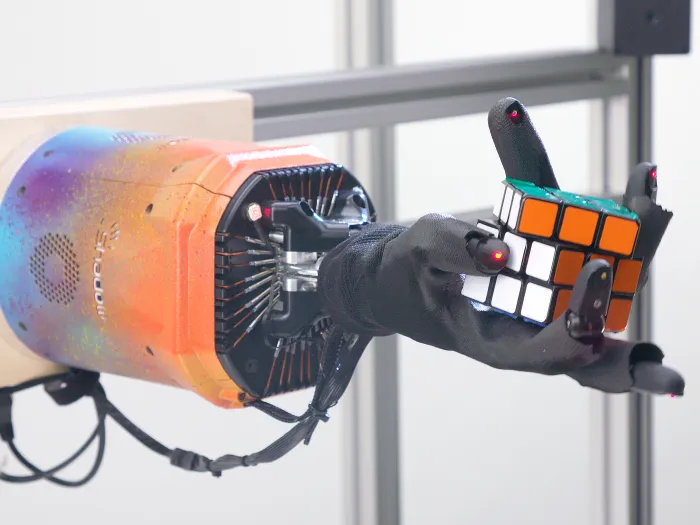
\includegraphics[width=0.55\linewidth,height=\textheight,keepaspectratio]{lecture1/images/openaidactyl.png}\\
Trained using PPO (Lecture 11)\\
\href{https://openai.com/index/solving-rubiks-cube/}{Link to Blog}

\section{Autonomous Vehicles}\label{autonomous-vehicles}

Self-driving cars rely on Reinforcement Learning to navigate complex
environments, optimize decision-making, and improve safety, often
incorporating PPO and deep learning to refine real-time control
strategies.

Partly trained using PPO (Lecture 11)

\section{Natural Language Processing}\label{natural-language-processing}

Reinforcement Learning from Human Feedback (RLHF) enhances AI language
models like ChatGPT, allowing them to refine responses based on user
interactions and align better with human preferences.

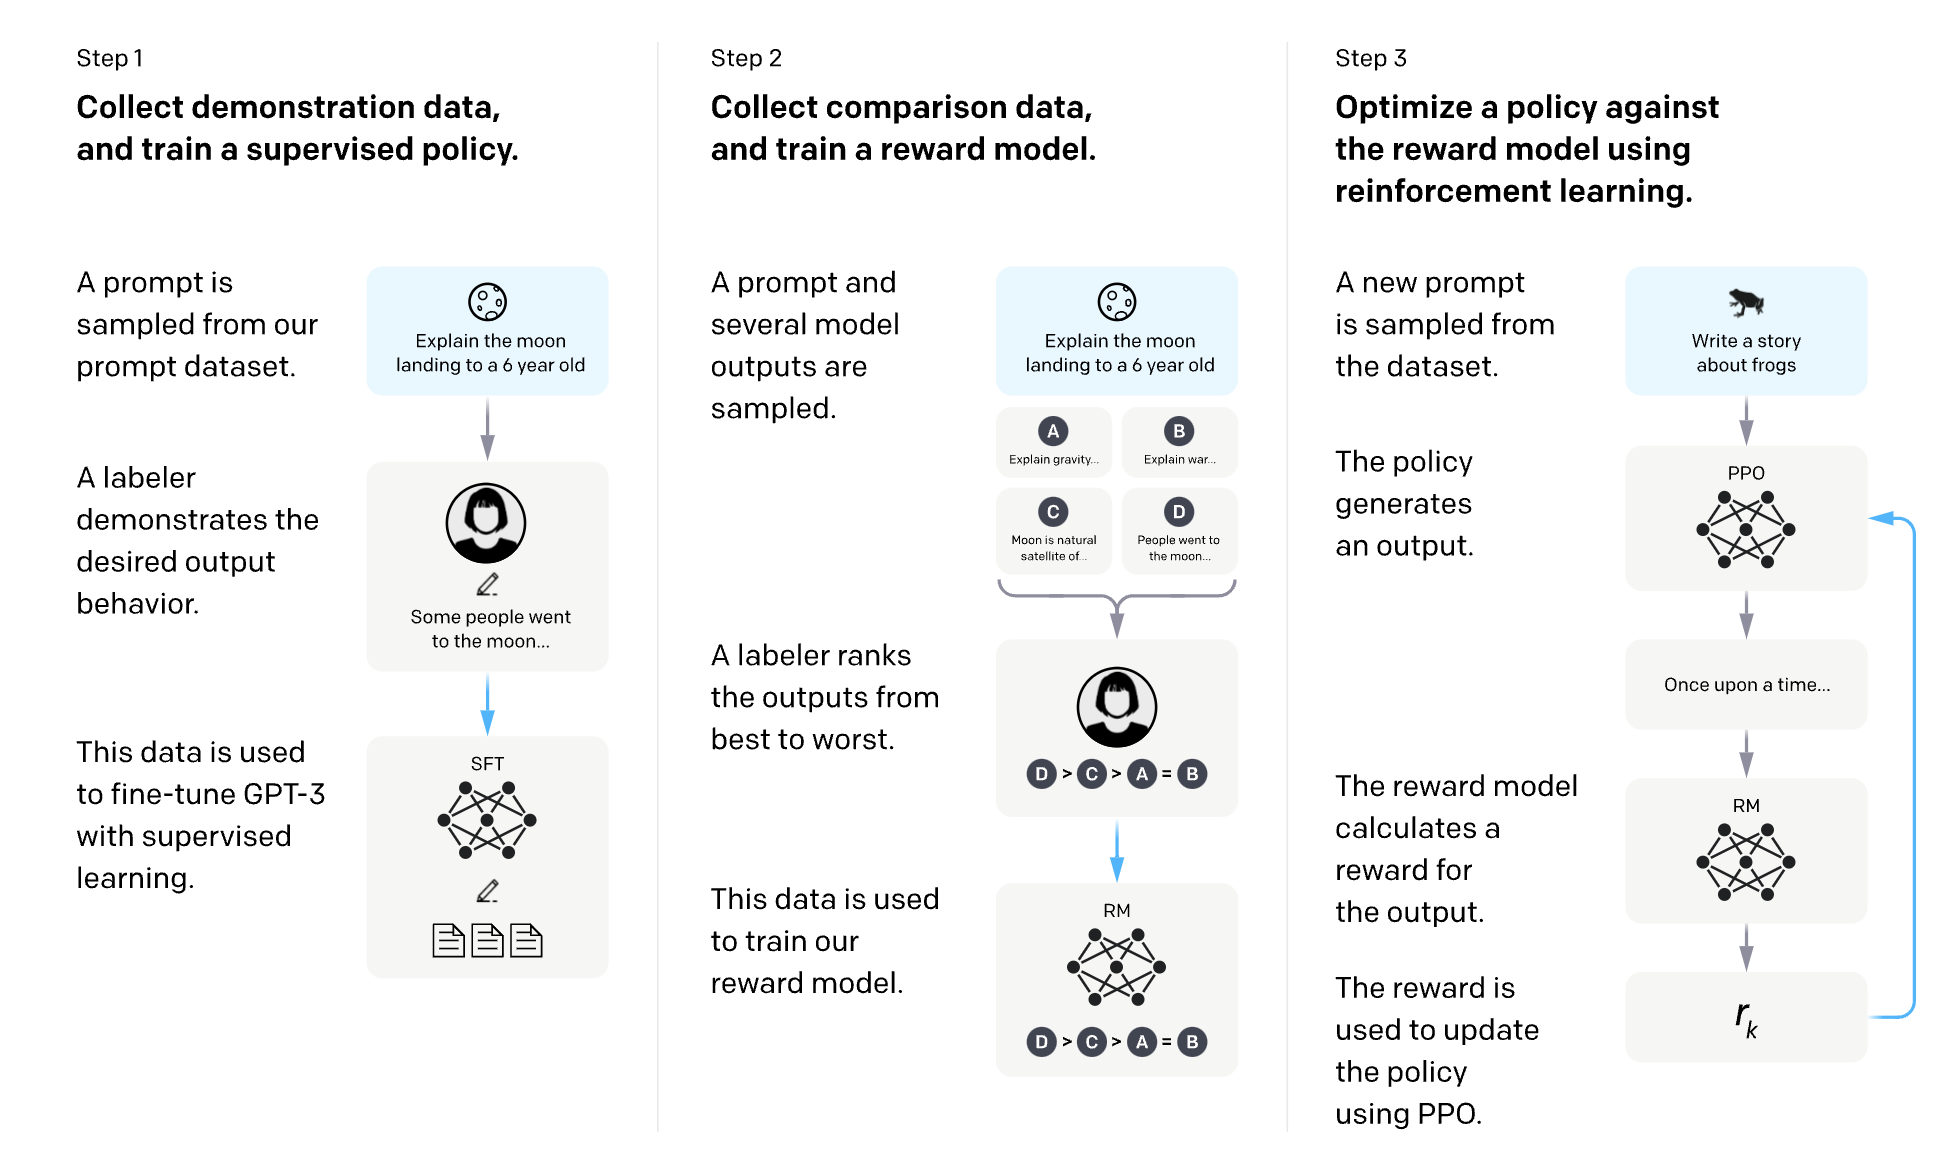
\includegraphics[width=0.7\linewidth,height=\textheight,keepaspectratio]{lecture1/images/rlhf.png}\\
Trained using PPO (Lecture 11)\\
\href{https://arxiv.org/pdf/2203.02155}{Link to Research Paper}

\section{Finance}\label{finance}

In financial markets, RL is applied to portfolio optimization,
algorithmic trading, and risk management, leveraging techniques like PPO
to make data-driven investment decisions.

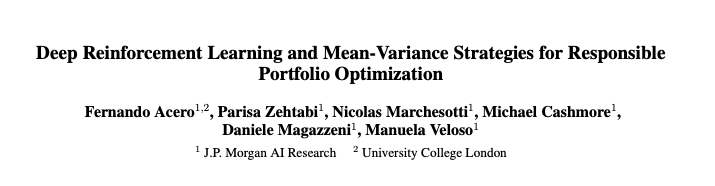
\includegraphics[width=0.7\linewidth,height=\textheight,keepaspectratio]{lecture1/images/jpmorgan.png}\\
Trained using PPO (Lecture 11)\\
\href{https://arxiv.org/pdf/2403.16667}{Link to Research Paper}

\chapter{1.4 How is Reinforcement Learning
Structured?}\label{how-is-reinforcement-learning-structured}

\begin{figure}[H]

{\centering \pandocbounded{\includegraphics[keepaspectratio]{index_files/mediabag/lecture1/images/SuggestedOutline.drawio.pdf}}

}

\caption{Taxonomy of Reinforcement Learning}

\end{figure}%

\part{Lecture 2: Mathematical Foundations}

\chapter{Learning Objectives}\label{learning-objectives}

\begin{tcolorbox}[enhanced jigsaw, colback=white, left=2mm, breakable, opacityback=0, bottomrule=.15mm, rightrule=.15mm, arc=.35mm, colframe=quarto-callout-note-color-frame, leftrule=.75mm, toprule=.15mm]

Learning Objectives for Lecture 2: Mathematical Foundations 🎯

\end{tcolorbox}

\begin{itemize}
\tightlist
\item
  Probability Theory:

  \begin{itemize}
  \tightlist
  \item
    Set Theory
  \item
    Axiomatic Probability
  \item
    Conditioning
  \item
    Independence
  \item
    Discrete Random Variables
  \item
    Continuous Random Variables
  \item
    Probability Distributions
  \end{itemize}
\end{itemize}

\begin{figure}[H]

{\centering \pandocbounded{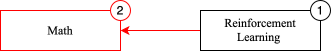
\includegraphics[keepaspectratio]{index_files/mediabag/lecture2/images/Lecture2.drawio.pdf}}

}

\caption{Taxonomy of Reinforcement Learning}

\end{figure}%

\chapter{2.1 Set Theory}\label{set-theory}

\begin{tcolorbox}[enhanced jigsaw, colback=white, left=2mm, breakable, opacityback=0, bottomrule=.15mm, rightrule=.15mm, arc=.35mm, colframe=quarto-callout-note-color-frame, leftrule=.75mm, toprule=.15mm]

The study of collections of objects, where elements either belong to a
set or they don't---simple, yet powerful! 🌍

\end{tcolorbox}

\section{Sets}\label{sets}

A \textbf{set} is a collection of things. The things are called
\textbf{elements} of a set.

\[
Colors = \{Red, Blue, Green\}
\]

\[
Numbers = \{1,2,3\}
\]

Sets can be \textbf{finite} or \textbf{infinite}.

\[
Some\ Even\ Integers = \{2,4,6\}
\]

\[
All\ Even\ Integers = \{..., -4, -2, 0, 2, 4, ...\}
\]

The number of elements in a set is called the \textbf{cardinality}.

\[
|Colors| = 3
\]

Two sets are \textbf{equal} if they share exactly the same elements.

\[
A = \{2,4,6\}, B = \{4,2,6\}, C = \{4,2,7\}
\]

\[
A = B
\] \[
A \neq C
\]

To express that \(2\) is an element of \(A\), we denote:

\[
2 \in A 
\] \[
\text{2 exists in A}
\]

\[
5 \notin A
\] \[
\text{5 does not exist in A}
\]

Some sets are so significant that we reserve special symbols for them:

\[
\emptyset = \{\} \quad \textbf{(empty set)}
\]

\[
\mathbb{N} = \{1, 2, 3, ... \} \quad \textbf{(natural numbers)}
\]

\[
\mathbb{Z} = \{..., -2, -1, 0, 1, 2, ... \} \quad \textbf{(integers)}
\]

\[
\mathbb{R} = \{..., -0.22,...,0,...,1,..., \pi, ... \} \quad \textbf{(real numbers)}
\]

We visualize \(\mathbb{R}\) as an infinitely long number line.

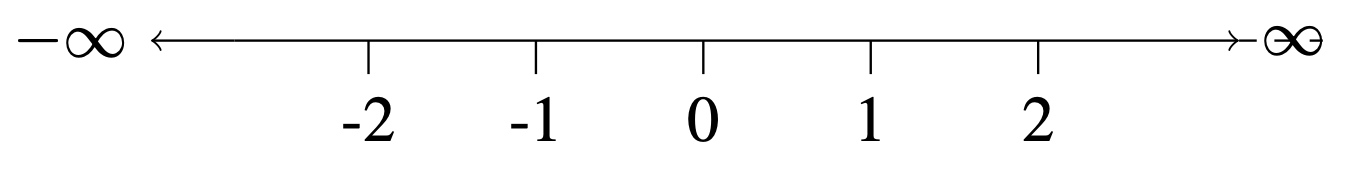
\includegraphics[width=0.5\linewidth,height=\textheight,keepaspectratio]{lecture2/images/numberline.png}

\section{Set-Builder Notation}\label{set-builder-notation}

A special notation called \textbf{set-builder notation} is used to
describe sets that are too big or complex to list between braces.

\[
All\ Even\ Integers_{1} = \{..., -4, -2, 0, 2, 4, ...\}
\]

\[
All\ Even\ Integers_{2} = \{2x: x \in \mathbb{Z} \}
\]

\[
\text{The set of all numbers of the form } 2x \text{ such that } x \in \mathbb{Z}
\]

\[
All\ Even\ Integers_{1} = All\ Even\ Integers_{2}
\]

\subsubsection{Exercise}\label{exercise}

Write the following sets in set-builder notation:

\begin{enumerate}
\def\labelenumi{\arabic{enumi}.}
\tightlist
\item
  \(\{ 2, 4, 8, 16, 32, 64, ... \}\)
\item
  \(\{ 0, 1, 4, 9, 16, 25, 36, ... \}\)
\item
  \(\{ 3, 4, 5, 6, 7, 8 \}\)
\end{enumerate}

\begin{tcolorbox}[enhanced jigsaw, opacityback=0, left=2mm, breakable, bottomtitle=1mm, rightrule=.15mm, colframe=quarto-callout-tip-color-frame, titlerule=0mm, colback=white, opacitybacktitle=0.6, toptitle=1mm, title=\textcolor{quarto-callout-tip-color}{\faLightbulb}\hspace{0.5em}{Solution}, colbacktitle=quarto-callout-tip-color!10!white, bottomrule=.15mm, arc=.35mm, coltitle=black, leftrule=.75mm, toprule=.15mm]

\begin{enumerate}
\def\labelenumi{\arabic{enumi}.}
\tightlist
\item
  \(\{ 2^x: x \in \mathbb{N} \}\)
\item
  \(\{ x^2: x \in \mathbb{Z} \}\)
\item
  \(\{ x \in \mathbb{Z}: 3 \le x \le 8 \}\)
\end{enumerate}

\end{tcolorbox}

\section{Subsets}\label{subsets}

Suppose \(A\) and \(B\) are sets. If every element of \(A\) is also an
element of \(B\), then we say \(A\) is a \textbf{subset} of \(B\),
denoted \(A \subseteq B\). We write \(A \not\subseteq B\) if \(A\) is
not a subset of \(B\), that is, if it is not true that every element of
\(A\) is also an element of \(B\). Thus \(A \not\subseteq B\) means that
there is at least one element of \(A\) that is not an element of \(B\).

\[
\mathbb{N} \subseteq \mathbb{Z} \subseteq \mathbb{R}
\]

\[
A = \{1,2\}, B = \{2,3,4\}
\] \[
A \not\subseteq B
\]

\subsubsection{Exercise}\label{exercise-1}

List all the subsets of the following sets:

\begin{enumerate}
\def\labelenumi{\arabic{enumi}.}
\tightlist
\item
  \(\{1,2,3\}\)
\item
  \(\{1,\{2,3\}\}\)
\item
  \(\{\mathbb{N}, \mathbb{Z}, \mathbb{R}\}\)
\end{enumerate}

\begin{tcolorbox}[enhanced jigsaw, opacityback=0, left=2mm, breakable, bottomtitle=1mm, rightrule=.15mm, colframe=quarto-callout-tip-color-frame, titlerule=0mm, colback=white, opacitybacktitle=0.6, toptitle=1mm, title=\textcolor{quarto-callout-tip-color}{\faLightbulb}\hspace{0.5em}{Solution}, colbacktitle=quarto-callout-tip-color!10!white, bottomrule=.15mm, arc=.35mm, coltitle=black, leftrule=.75mm, toprule=.15mm]

\begin{enumerate}
\def\labelenumi{\arabic{enumi}.}
\tightlist
\item
  \(\{\}, \{1\}, \{2\}, \{3\}, \{1,2\}, \{1,3\}, \{2,3\}, \{1,2,3\}\)
\item
  \(\{\}, \{1\}, \{\{2,3\}\}, \{1,\{2,3\}\}\)
\item
  \(\{\}, \{\mathbb{N}\}, \{\mathbb{Z}\}, \{\mathbb{R}\}, \{\mathbb{N},\mathbb{Z}\}, \{\mathbb{N},\mathbb{R}\}, \{\mathbb{Z},\mathbb{R}\}, \{\mathbb{N},\mathbb{Z},\mathbb{R}\}\)
\end{enumerate}

\end{tcolorbox}

\section{Union, Intersection, and
Difference}\label{union-intersection-and-difference}

Suppose \(A\) and \(B\) are sets.

A \textbf{union} of \(A\) and \(B\) is the set: \[
A \cup B = \{x: x \in A \text{ or } x \in B \}
\]

A \textbf{intersection} of \(A\) and \(B\) is the set: \[
A \cap B = \{x: x \in A \text{ and } x \in B \}
\]

A \textbf{difference} of \(A\) and \(B\) is the set: \[
A - B = \{x: x \in A \text{ and } x \notin B \}
\]

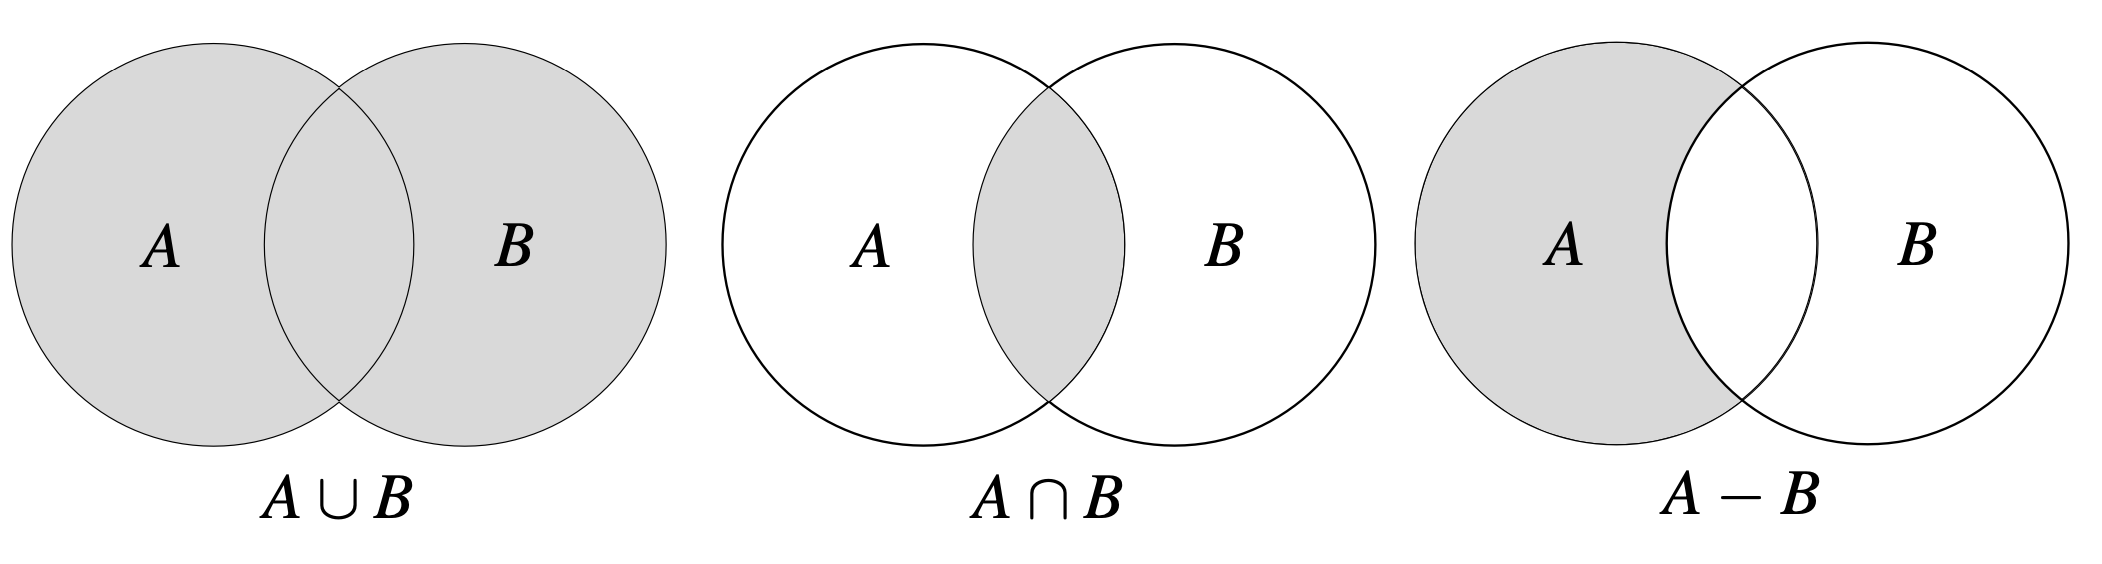
\includegraphics[width=0.75\linewidth,height=\textheight,keepaspectratio]{lecture2/images/union-intersection-complement.png}

\subsubsection{Exercise}\label{exercise-2}

Shade in the region matching the expression:

\begin{enumerate}
\def\labelenumi{\arabic{enumi}.}
\tightlist
\item
  \((A \cap B) \cap C\)
\item
  \((A \cup B) \cap C\)
\item
  \((A \cup B) - C\)
\end{enumerate}

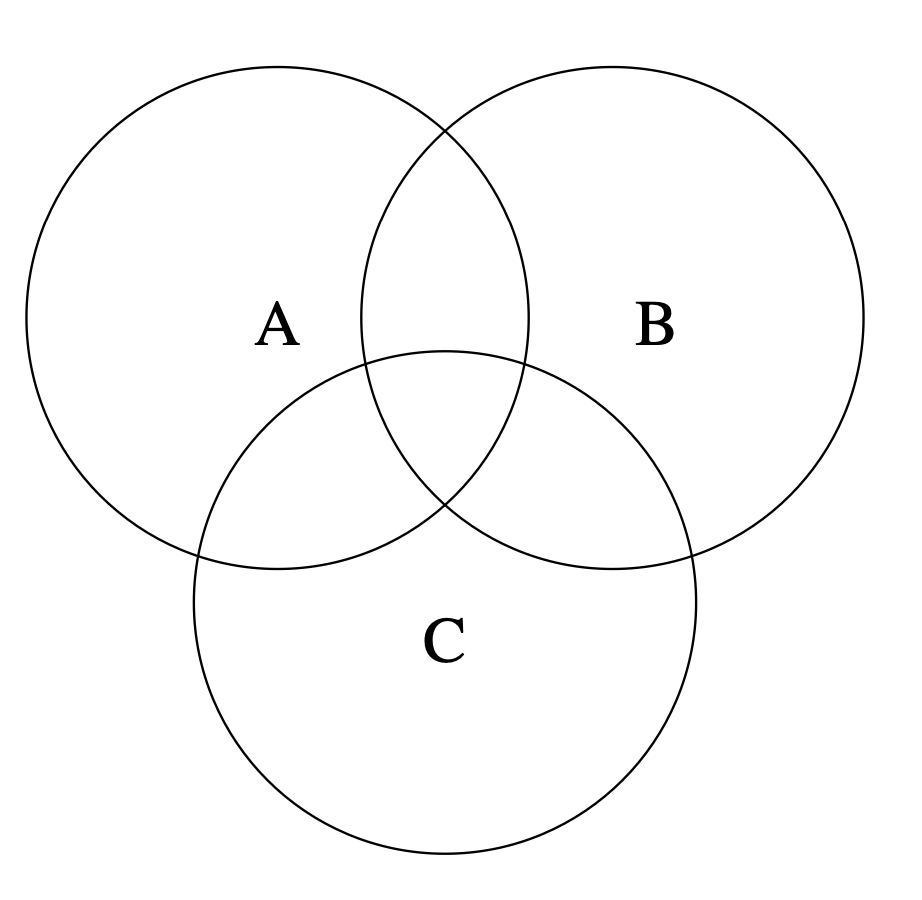
\includegraphics[width=0.35\linewidth,height=\textheight,keepaspectratio]{lecture2/images/union-intersection-complement-ex.png}

\begin{tcolorbox}[enhanced jigsaw, opacityback=0, left=2mm, breakable, bottomtitle=1mm, rightrule=.15mm, colframe=quarto-callout-tip-color-frame, titlerule=0mm, colback=white, opacitybacktitle=0.6, toptitle=1mm, title=\textcolor{quarto-callout-tip-color}{\faLightbulb}\hspace{0.5em}{Solution}, colbacktitle=quarto-callout-tip-color!10!white, bottomrule=.15mm, arc=.35mm, coltitle=black, leftrule=.75mm, toprule=.15mm]

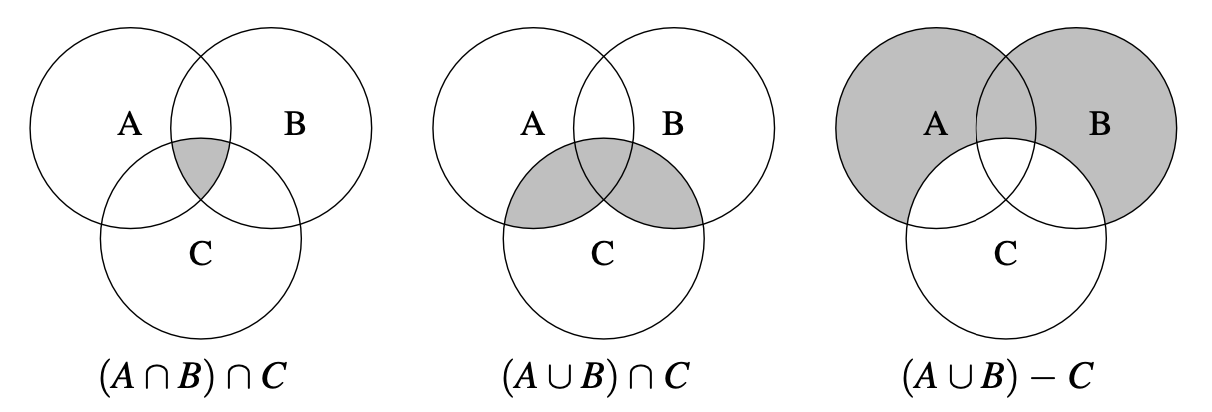
\includegraphics[width=0.75\linewidth,height=\textheight,keepaspectratio]{lecture2/images/union-intersection-complement-ans.png}

\end{tcolorbox}

\section{Complements}\label{complements}

Suppose \(A\) is a set. A \textbf{universal set} is a larger set that
encompasses other sets. The \textbf{complement} of \(A\), denoted
\(\bar{A}\), is the set \(\bar{A} = U - A\).

\[
P = \{2, 3, 5, 7, ...\} \quad \textbf{(prime numbers)}
\]

\[
\bar{P} = \mathbb{N} - P = \{1, 4, 6, ...\}
\]

\subsubsection{Exercise}\label{exercise-3}

Find \(\bar{A}\):

\[
A = \{1,2,3\}, U = \{0,1,2,3,4,5\}
\]

\begin{tcolorbox}[enhanced jigsaw, opacityback=0, left=2mm, breakable, bottomtitle=1mm, rightrule=.15mm, colframe=quarto-callout-tip-color-frame, titlerule=0mm, colback=white, opacitybacktitle=0.6, toptitle=1mm, title=\textcolor{quarto-callout-tip-color}{\faLightbulb}\hspace{0.5em}{Solution}, colbacktitle=quarto-callout-tip-color!10!white, bottomrule=.15mm, arc=.35mm, coltitle=black, leftrule=.75mm, toprule=.15mm]

\[
\bar{A} = \{0, 4, 5\}
\]

\end{tcolorbox}

\chapter{2.2 Axiomatic Probability}\label{axiomatic-probability}

\begin{tcolorbox}[enhanced jigsaw, colback=white, left=2mm, breakable, opacityback=0, bottomrule=.15mm, rightrule=.15mm, arc=.35mm, colframe=quarto-callout-note-color-frame, leftrule=.75mm, toprule=.15mm]

A formal framework that defines probability using three fundamental
rules, ensuring consistency in measuring uncertainty. 🎲

\end{tcolorbox}

\section{Methodology}\label{methodology}

Steps to perform a probabilistic model:

\begin{enumerate}
\def\labelenumi{\arabic{enumi}.}
\tightlist
\item
  Specify sample space.
\item
  Define probability law (must align with probability axioms).
\item
  Identify event of interest.
\item
  Calculate\ldots{}
\end{enumerate}

\section{Sample Space}\label{sample-space}

A \textbf{sample space} is a set of all possible outcomes from an
experiment.

\[
Sample \ Space = \{Heads, Tails\}
\]

An \textbf{experiment} is any procedure that can be repeated and has a
well-defined set of outcomes.

\[
Flipping \ a \ fair \ coin 
\]

An \textbf{outcome} is the end result of an experiment, or an element in
the sample space.

\[
Heads  
\]

\section{Illustration: Discrete Sample
Space}\label{illustration-discrete-sample-space}

\textbf{Experiment:} Rolling two fair die at the same time.

\[ 
Sample \ Space = \{ (x, y) : x,y \in \mathbb{N}, 1 \leq x, y \leq 6  \} 
\]

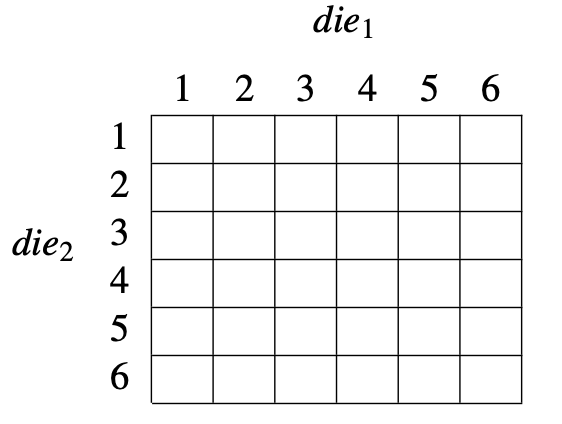
\includegraphics[width=0.3\linewidth,height=\textheight,keepaspectratio]{lecture2/images/discrete-axiomatic.png}

\section{Illustration: Continuous Sample
Space}\label{illustration-continuous-sample-space}

\textbf{Experiment:} Measure two continuous variables in the range
\([0,1]\)

\[ Sample\ Space = \{ (x, y) : x,y \in \mathbb{R}, 0 \leq x, y \leq 1  \} \]

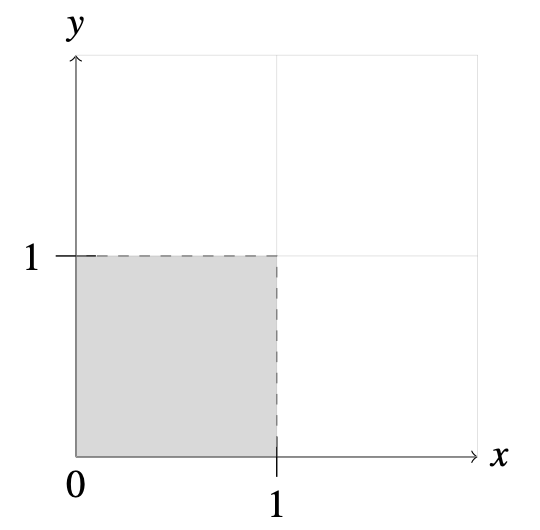
\includegraphics[width=0.3\linewidth,height=\textheight,keepaspectratio]{lecture2/images/continuous-axiomatic.png}

\section{Events and Experiment}\label{events-and-experiment}

An \textbf{event} is a subset of the sample space. Events are important
because they ultimately get assigned probabilities.

\textbf{Experiment:} Rolling a die once.

\[ 
Sample \ Space = \{1,2,3,4,5,6\}
\]

What is the event of rolling a \(1\)?

\[
\{1\} \subseteq \{1,2,3,4,5,6\}
\]

What is the event of rolling an odd number?

\[
\{1, 3, 5\} \subseteq \{1,2,3,4,5,6\}
\]

\section{Probability Axioms and Probability
Law}\label{probability-axioms-and-probability-law}

Kolmogorov \textbf{probability axioms} are the foundations of axiomatic
probability theory:

\begin{enumerate}
\def\labelenumi{\arabic{enumi}.}
\tightlist
\item
  \textbf{Nonnegativity:} \(P(Event) \geq 0\)
\item
  \textbf{Normalization:} \(P(Sample\ Space) = 1\)
\item
  \textbf{Additivity:} If
  \(A \cap B = \emptyset, P(A \cup B) = P(A) + P(B)\)
\end{enumerate}

\textbf{Probability laws} are additional axioms mathematically derived
from Kolmogorov probability axioms.

\subsubsection{Exercise}\label{exercise-4}

\textbf{Experiment}: Rolling two fair die at the same time.

Let all outcomes be equally likely.

\[ 
P(A) = \frac{|A|}{|Sample\ Space|}
\]

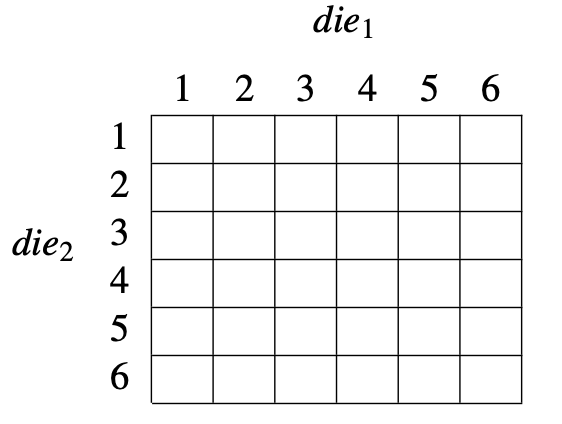
\includegraphics[width=0.3\linewidth,height=\textheight,keepaspectratio]{lecture2/images/discrete-axiomatic.png}

Find the following probabilities:

\begin{enumerate}
\def\labelenumi{\arabic{enumi}.}
\tightlist
\item
  \(P(die_1 = 1)\)
\item
  \(P(max(die_1, die_2) = 2)\)
\end{enumerate}

\begin{tcolorbox}[enhanced jigsaw, opacityback=0, left=2mm, breakable, bottomtitle=1mm, rightrule=.15mm, colframe=quarto-callout-tip-color-frame, titlerule=0mm, colback=white, opacitybacktitle=0.6, toptitle=1mm, title=\textcolor{quarto-callout-tip-color}{\faLightbulb}\hspace{0.5em}{Solution}, colbacktitle=quarto-callout-tip-color!10!white, bottomrule=.15mm, arc=.35mm, coltitle=black, leftrule=.75mm, toprule=.15mm]

\begin{enumerate}
\def\labelenumi{\arabic{enumi}.}
\tightlist
\item
  \(P(die_1 = 1) = \frac{6}{36} \approx 0.1\bar{6}\)
\item
  \(P(max(die_1, die_2) = 2) = \frac{2}{36} \approx 0.0\bar{5}\)
\end{enumerate}

\end{tcolorbox}

\subsubsection{Exercise}\label{exercise-5}

\textbf{Experiment}: Measure two continuous variables in the range
\([0,1]\)

\[ 
Sample\ Space = \{ (x, y) : x,y \in \mathbb{R}, 0 \leq x, y \leq 1  \} 
\]

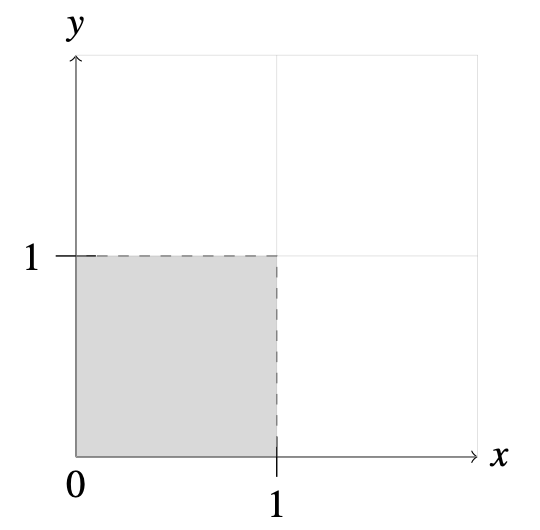
\includegraphics[width=0.3\linewidth,height=\textheight,keepaspectratio]{lecture2/images/continuous-axiomatic.png}

Find the following probabilities:

\begin{enumerate}
\def\labelenumi{\arabic{enumi}.}
\tightlist
\item
  \(P(x = 0.5 , y = 0.5)\)
\item
  \(P(x+y \geq 1)\)
\end{enumerate}

\begin{tcolorbox}[enhanced jigsaw, opacityback=0, left=2mm, breakable, bottomtitle=1mm, rightrule=.15mm, colframe=quarto-callout-tip-color-frame, titlerule=0mm, colback=white, opacitybacktitle=0.6, toptitle=1mm, title=\textcolor{quarto-callout-tip-color}{\faLightbulb}\hspace{0.5em}{Solution}, colbacktitle=quarto-callout-tip-color!10!white, bottomrule=.15mm, arc=.35mm, coltitle=black, leftrule=.75mm, toprule=.15mm]

\begin{enumerate}
\def\labelenumi{\arabic{enumi}.}
\tightlist
\item
  \(P(x = 0.5 , y = 0.5) = 0\)
\item
  \(P(x+y \geq 1) = 0.5\)
\end{enumerate}

\end{tcolorbox}

\chapter{2.3 Conditioning}\label{conditioning}

\begin{tcolorbox}[enhanced jigsaw, colback=white, left=2mm, breakable, opacityback=0, bottomrule=.15mm, rightrule=.15mm, arc=.35mm, colframe=quarto-callout-note-color-frame, leftrule=.75mm, toprule=.15mm]

A way to update probabilities when given new information, refining our
understanding of how likely an event is. 🤔

\end{tcolorbox}

\section{Conditional Probability}\label{conditional-probability}

Suppose \(A\) and \(B\) are events. \textbf{Conditional probability} is
the likelihood of an event occurring given that we know another event
has occurred.

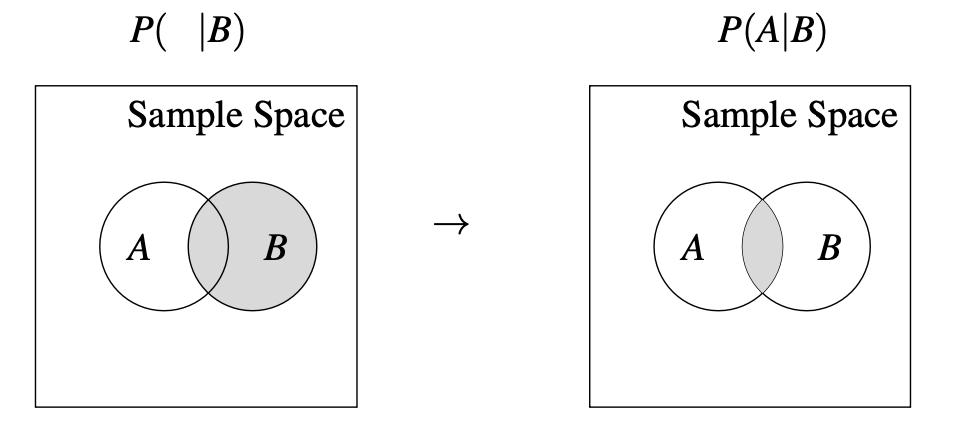
\includegraphics[width=0.55\linewidth,height=\textheight,keepaspectratio]{lecture2/images/condprob.png}

\[ 
P(A|B) = \frac{P(A \cap B)}{P(B)} 
\]

Intuition: conditioned event becomes the new sample space. If
\(P(B) \neq 0\), then the probability of the intersection normalized by
the conditioned space. Else \(P(B) = 0\), then \(P(A|B)\) is undefined.

\section{Product Rule}\label{product-rule}

Suppose \(A\) and \(B\) are events. The \textbf{product rule} states
that the probability of two events \(A\) and \(B\) occurring together
\(A \cap B\) is given by the probability of one event occurring given
the other \(P(A|B)\) or \(P(B|A)\) multiplied by the probability of the
other event.

\[ 
P(A \cap B) = P(A|B) P(B) = P(B|A) P(A) 
\]

\section{Total Probability Theorem}\label{total-probability-theorem}

Suppose \(A_{1,...,n}\) and \(B\) are sets. The \textbf{total
probability theorem} allows us to compute the likelihood of an event by
summing over conditional probabilities of different partitions of the
sample space.

\[ 
P(B) = P(B|A_1) P(A_1) + P(B|A_2) P(A_2) + P(B|A_3) P(A_3)
\]

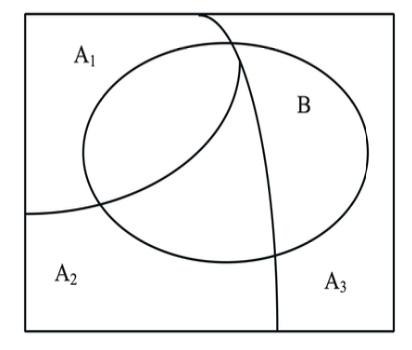
\includegraphics[width=0.3\linewidth,height=\textheight,keepaspectratio]{lecture2/images/totalcondprob.pdf}

In general terms:

\[
P(B) = P(B|A_1) P(A_1) + ... + P(B|A_n) P(A_n)
\]

\subsubsection{Exercise}\label{exercise-6}

\textbf{Experiment}: Classifying emails as spam \(S\) or not spam \(NS\)
based on the word \(W\) or not the word \(NW\) ``free''.

\[
P(S) = 0.4
\]

\[
P(NS) = 0.6
\]

\[
P(W|S) = 0.7
\]

\[
P(W|NS) = 0.1
\]

Find the probability of \(P(S|W)\):

\begin{tcolorbox}[enhanced jigsaw, opacityback=0, left=2mm, breakable, bottomtitle=1mm, rightrule=.15mm, colframe=quarto-callout-tip-color-frame, titlerule=0mm, colback=white, opacitybacktitle=0.6, toptitle=1mm, title=\textcolor{quarto-callout-tip-color}{\faLightbulb}\hspace{0.5em}{Solution}, colbacktitle=quarto-callout-tip-color!10!white, bottomrule=.15mm, arc=.35mm, coltitle=black, leftrule=.75mm, toprule=.15mm]

\[
P(S|W) = \frac{P(S \cap W)}{P(W)} = \underbrace{\frac{P(W|S)P(S)}{P(W|S)P(S) + P(W|NS)P(NS)}}_{Bayes' \ Theorem} = \frac{0.7 * 0.4}{0.7 * 0.4 + 0.1 * 0.6} = 0.82
\]

\end{tcolorbox}

\chapter{2.4 Independence}\label{independence}

\begin{tcolorbox}[enhanced jigsaw, colback=white, left=2mm, breakable, opacityback=0, bottomrule=.15mm, rightrule=.15mm, arc=.35mm, colframe=quarto-callout-note-color-frame, leftrule=.75mm, toprule=.15mm]

A property where two events do not influence each other, meaning the
occurrence of one tells us nothing about the other. 🔗

\end{tcolorbox}

\section{Independent Events}\label{independent-events}

Suppose \(A\) and \(B\) are two events. Two events are
\textbf{independent} if the occurrence of event \(B\) provides no
information about the occurrence of event \(A\):

\[ 
P(A|B) = P(A) 
\]

Another definition of independence:

\[ 
P(A \cap B) = P(A) P(B)
\]

For multiple events:

\[ 
P(A_{1} \cap A_{2} \cap ... A_{n}) = P(A_{1}) P(A_{2}) ... P(A_{n})
\]

\section{Conditioning and
Independence}\label{conditioning-and-independence}

Suppose \(A\), \(B\), and \(C\) are events. If \(A\) and \(B\) are
independent, conditioning on \(C\) may remove that independence. When we
condition on \(C\), events \(A\) and \(B\) may no longer be independent.

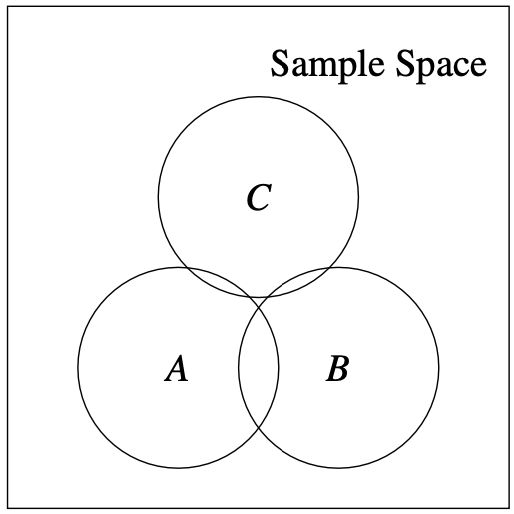
\includegraphics[width=0.3\linewidth,height=\textheight,keepaspectratio]{lecture2/images/condind.png}

\subsubsection{Exercise}\label{exercise-7}

The king comes from a family of two children. What is the probability
that his sibling is female \(F\) and not male \(M\)?

Let all outcomes be equally likely.

\begin{tcolorbox}[enhanced jigsaw, opacityback=0, left=2mm, breakable, bottomtitle=1mm, rightrule=.15mm, colframe=quarto-callout-tip-color-frame, titlerule=0mm, colback=white, opacitybacktitle=0.6, toptitle=1mm, title=\textcolor{quarto-callout-tip-color}{\faLightbulb}\hspace{0.5em}{Solution}, colbacktitle=quarto-callout-tip-color!10!white, bottomrule=.15mm, arc=.35mm, coltitle=black, leftrule=.75mm, toprule=.15mm]

\[
Sample \ Space = \{(FF), (FM), (MF), (MM)\} = \{(\not F \not F), (FM), (MF), (MM)\}
\]

\[
P(F|M) = \frac{P(F \cap M)}{M} = \frac{2}{3} \approx 0.6\bar{6}
\]

\end{tcolorbox}

\chapter{2.5 Discrete Random Variables}\label{discrete-random-variables}

\begin{tcolorbox}[enhanced jigsaw, colback=white, left=2mm, breakable, opacityback=0, bottomrule=.15mm, rightrule=.15mm, arc=.35mm, colframe=quarto-callout-note-color-frame, leftrule=.75mm, toprule=.15mm]

A type of variable that takes distinct, countable values, often used to
model finite outcomes. 📊

\end{tcolorbox}

\section{Discrete Random Variable}\label{discrete-random-variable}

A \textbf{discrete random variable} is a mapping \(X\) of all of the
outcomes of a sample space to numerical values \(x \in \mathbb{Z}\).

\[
X: Outcome \in Sample \ Space \to x \in \mathbb{Z}
\]

\section{Probability Mass Function
(PMF)}\label{probability-mass-function-pmf}

A \textbf{probability mass function (PMF)} is a mapping of values \(x\)
of discrete random variables \(X\) to probabilities \([0,1]\).

\[
p_{X}(x) = P(X = x)
\]

PMF has properties: \[
p_{X}(x) \geq 0, \quad \sum_{x} p_{X}(x) = 1
\]

\section{Cumulative Distribution Function
(CDF)}\label{cumulative-distribution-function-cdf}

The \textbf{cumulative distribution function (CDF)} for discrete random
variables is defined as:

\[
F_{X}(x) = P(X \leq x) = \sum_{k \leq x} p_{X}(k)
\]

Relation to PMF: \[
p_{X}(x) = \frac{dF_{X}(x)}{dx}
\]

\[
F_{X}(x) = \sum_{k \leq x}p_{X}(k)
\]

\section{Illustration: PMF and CDF}\label{illustration-pmf-and-cdf}

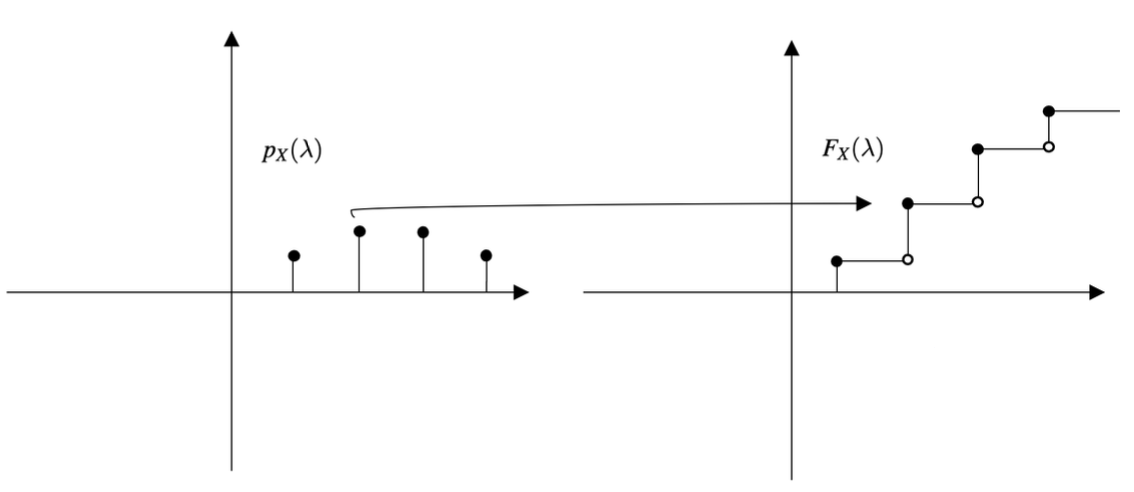
\includegraphics[width=0.75\linewidth,height=\textheight,keepaspectratio]{lecture2/images/pdf-cdf.png}

\section{Expectation and Variance of
PMFs}\label{expectation-and-variance-of-pmfs}

Discrete \textbf{expectation}, or mean, is the average numerical value
that the discrete random variable takes over the PMF. \[
E[X] = \sum_{x} x \ p_{X}(x)
\]

Discrete \textbf{variance} is the expected squared difference from the
mean of a PMF. \[
Var[X] = E[(X - E[X])^{2}] = \sum_{x}(x - E[X])^2 p_{X}(x)
\]

\section{Joint and Marginal PMFs}\label{joint-and-marginal-pmfs}

The \textbf{joint PMF} calculates the intersection of two discrete
random variables: \[
p_{X,Y}(x_{1},x_{2}) = P(X = x_{1}, Y = x_{2})
\]

From the previous definition we can also compute the \textbf{marginal
PMF} for a particular random variable: \[
p_{X}(x_{1}) = \sum_{x_{2}} p_{X,Y}(X = x_{1},Y = x_{2})
\]

\section{Conditional Expectation of
PMFs}\label{conditional-expectation-of-pmfs}

The \textbf{conditional PMF} gives the probability distribution of a
discrete random variable given that another variable has a specific
value. \[
p_{X|Y}(x_{1}| x_{2}) = \frac{p_{X,Y}(x_{1}, x_{2})}{p_{Y}(x_{2})}
\]

The \textbf{conditional expectation} is the expected value of a discrete
random variable given that another variable is fixed at a specific
value. \[
E[X| Y = x_{2}] = \sum_{x_{1}} x_{1} \frac{p_{X,Y}(x_{1}, x_{2})}{p_{Y}(x_{2})}
\]

\section{Independence}\label{independence-1}

Two discrete random variables are \textbf{independent} if:

\[
p_{X,Y}(x_{1}, x_{2}) = p_{X}(x_{1}) p_{Y}(x_{2})
\]

For multiple discrete random variables: \[
p_{X_{1},...,X_{n}}(x_{1}, ..., x_{n}) = p_{X_{1}}(x_{1}) ... \ p_{X_{n}}(x_{n})
\]

\chapter{2.6 Continuous Random
Variables}\label{continuous-random-variables}

\begin{tcolorbox}[enhanced jigsaw, colback=white, left=2mm, breakable, opacityback=0, bottomrule=.15mm, rightrule=.15mm, arc=.35mm, colframe=quarto-callout-note-color-frame, leftrule=.75mm, toprule=.15mm]

A variable that can take any value within a range, requiring calculus to
describe its probabilities. 📈

\end{tcolorbox}

\section{Continuous Random Variable}\label{continuous-random-variable}

A \textbf{continuous random variable} is a mapping \(X\) of all the
events of a sample space to numerical values \(x \in \mathbb{R}\). \[ 
X: Event \in Sample \ Space \to x \in \mathbb{R} 
\]

\section{Probability Density Function
(PDF)}\label{probability-density-function-pdf}

A \textbf{probability density function (PDF)} is a mapping of values
\(x\) of intervals of continuous random variables \(X\) to probabilities
\([0,1]\).

\[ 
P(a \leq X \leq b) = \int_{a}^{b} f_{X}(x) \ dx 
\]

PDF has properties: \[
f_{X}(x) \geq 0, \ \int_{-\infty}^{\infty} f_{X}(x) \ dx = 1
\]

\section{Cumulative Distribution Function
(CDF)}\label{cumulative-distribution-function-cdf-1}

The \textbf{cumulative distribution function (CDF)} for continuous
random variables is defined as:

\[ F_{X}(x) = P(X \leq x) = \int_{-\infty}^{x} f_{X}(u) \ du \]

Relation to PDF:

\[
f_{X}(x) = \frac{dF_{X}(x)}{dx}
\] \[
F_{X}(x) = \int_{-\infty}^{x} f_{X}(u) \ du
\]

\section{Illustration: PDF and CDF}\label{illustration-pdf-and-cdf}

\includegraphics[width=0.75\linewidth,height=\textheight,keepaspectratio]{index_files/mediabag/lecture2/images/pdfcdf.drawio.pdf}

\section{Expectation and Variance of
PDFs}\label{expectation-and-variance-of-pdfs}

Continuous \textbf{expectation}, or mean, is the average numerical value
that the continuous random variable takes over the PDF. \[ 
E[X] = \int_{-\infty}^{\infty} x \ f_{X}(x) dx 
\]

Continuous \textbf{variance} is the expected squared difference from the
mean of a PDF. \[ 
\text{Var}[X] = E[(X - E[X])^{2}] = \int_{-\infty}^{\infty} (x - E[X])^2 \ f_{X}(x) dx 
\]

\section{Joint and Marginal PDFs}\label{joint-and-marginal-pdfs}

The \textbf{joint PDF} calculates the intersection of two continuous
random variables: \[ 
P((X,Y) \in A) = \int \int_{A} f_{X,Y}(x_{1}, x_{2}) dx_{1} \ dx_{2} 
\]

From the previous definition we can also compute the \textbf{marginal
PDF} for a particular random variable:

\[
f_{X}(x_{1}) = \int_{-\infty}^{\infty} f_{X,Y}(x_{1}, x_{2}) dx_{2}
\]

\[
f_{Y}(x_{2}) = \int_{-\infty}^{\infty} f_{X,Y}(x_{1},x_{2}) dx_{1}
\]

\section{Conditional Expectation of
PDFs}\label{conditional-expectation-of-pdfs}

The \textbf{conditional PDF} gives the probability distribution of a
continuous random variable given that another variable has a specific
value. \[ 
f_{X|Y}(x_{1}| x_{2}) = \frac{f_{X,Y}(x_{1}, x_{2})}{f_{Y}(x_{2})} 
\]

The \textbf{conditional expectation} is the expected value of a
continuous random variable given that another variable is fixed at a
specific value. \[ 
\mathbb{E}[X| Y = x_{2}] = \int_{x_{1} \in X} x_{1} \frac{f_{X,Y}(x_{1}, x_{2})}{f_{Y}(x_{2})} dx_{1} 
\]

\section{Independence}\label{independence-2}

Two continuous random variables are \textbf{independent} if: \[ 
f_{X,Y}(x_{1}, x_{2}) = f_{X}(x_{1}) f_{Y}(x_{2}) 
\]

This can be extended to multiple random variables: \[ 
f_{X_{1},...,X{n}}(x_{1}, ..., x_{n}) = f_{X_{1}}(x_{1}) ... \ f_{X_{n}}(x_{n}) 
\]

\chapter{2.7 Probability Distributions}\label{probability-distributions}

\begin{tcolorbox}[enhanced jigsaw, colback=white, left=2mm, breakable, opacityback=0, bottomrule=.15mm, rightrule=.15mm, arc=.35mm, colframe=quarto-callout-note-color-frame, leftrule=.75mm, toprule=.15mm]

A function that assigns probabilities to outcomes, defining the overall
behavior of a random process. 🤓

\end{tcolorbox}

\section{Bernoulli Distribution}\label{bernoulli-distribution}

\[
p_{X}(x) =
\begin{cases}
    p & \text{if } x = 1, \\
    q = 1-p & \text{if } x = 0.
\end{cases}
\]

\begin{itemize}
\tightlist
\item
  The discrete random variable can take value \(1\) with probability
  \(p\) or value \(0\) with probability \(q = 1 - p\)
\item
  Not to be confused with the binomial distribution, since only one
  trial is being conducted.
\item
  \(\mathbb{E}[X] = p\)
\item
  \(Var[X] = pq\)
\end{itemize}

\phantomsection\label{observable}
\begin{Shaded}
\begin{Highlighting}[]
\NormalTok{//| echo: false}
\NormalTok{//| layout{-}align: center}

\NormalTok{viewof p = Inputs.range([0, 1], \{}
\NormalTok{  step: 0.01,}
\NormalTok{  value: 0.5,}
\NormalTok{  label: tex\textasciigrave{}p\textasciigrave{},}
\NormalTok{  width: 200}
\NormalTok{\})}

\NormalTok{data = \{}
\NormalTok{  return [}
\NormalTok{    \{outcome: "0", probability: 1 {-} p\},}
\NormalTok{    \{outcome: "1", probability: p\}}
\NormalTok{  ];}
\NormalTok{\}}

\NormalTok{Plot.plot(\{}
\NormalTok{  style: "overflow: visible; display: block; margin: 0 auto;",}
\NormalTok{  width: 600,}
\NormalTok{  height: 400,}
\NormalTok{  y: \{}
\NormalTok{    grid: true,}
\NormalTok{    label: "Probability",}
\NormalTok{    domain: [0, 1]}
\NormalTok{  \},}
\NormalTok{  x: \{}
\NormalTok{    label: "Outcome",}
\NormalTok{    padding: 0.2}
\NormalTok{  \},}
\NormalTok{  marks: [}
\NormalTok{    Plot.barY(data, \{}
\NormalTok{      x: "outcome",}
\NormalTok{      y: "probability",}
\NormalTok{      fill: "steelblue"}
\NormalTok{    \}),}
\NormalTok{    Plot.ruleY([0])}
\NormalTok{  ]}
\NormalTok{\})}

\NormalTok{html\textasciigrave{}\textless{}div style="text{-}align: center; margin{-}top: 1em;"\textgreater{}}
\NormalTok{  \textless{}p\textgreater{}$\{tex\textasciigrave{}\textbackslash{}mathbb\{E\}[X] =\textasciigrave{}\} $\{p.toFixed(3)\}\textless{}/p\textgreater{}}
\NormalTok{  \textless{}p\textgreater{}$\{tex\textasciigrave{}\textbackslash{}text\{Var\}(X) =\textasciigrave{}\} $\{(p * (1{-}p)).toFixed(3)\}\textless{}/p\textgreater{}}
\NormalTok{\textless{}/div\textgreater{}\textasciigrave{}}
\end{Highlighting}
\end{Shaded}

\subsection{Python Code: Bernoulli
Distribution}\label{python-code-bernoulli-distribution}

To create Bernoulli distributed data using \texttt{numpy}:

\begin{Shaded}
\begin{Highlighting}[]
\ImportTok{import}\NormalTok{ numpy }\ImportTok{as}\NormalTok{ np}

\NormalTok{interval }\OperatorTok{=}\NormalTok{ [}\DecValTok{0}\NormalTok{,}\DecValTok{1}\NormalTok{]}
\NormalTok{size }\OperatorTok{=}\NormalTok{ (}\DecValTok{1000}\NormalTok{,}\DecValTok{1}\NormalTok{)}
\NormalTok{p }\OperatorTok{=}\NormalTok{ [}\DecValTok{1}\OperatorTok{{-}}\FloatTok{0.5}\NormalTok{, }\FloatTok{0.5}\NormalTok{]}

\NormalTok{data }\OperatorTok{=}\NormalTok{ np.random.choice(interval, size, p }\OperatorTok{=}\NormalTok{ p)}
\end{Highlighting}
\end{Shaded}

\section{Gaussian Distribution}\label{gaussian-distribution}

\[
f_{X}(x)=\frac{1}{\sqrt{2\pi\sigma^{2} }}e^{-\frac{(x-\mu)^{2}}{2\sigma^{2}}}
\]

\begin{itemize}
\tightlist
\item
  Used frequently to represent real-valued random variables whose
  distributions are not known.
\item
  Its importance is derived from the \textbf{central limit theorem} that
  states, under some conditions, the average of many samples of a random
  variable is itself a random variable that converges to a Gaussian
  distribution as it increases.
\item
  \(E[X] = \mu\)
\item
  \(Var[X] = \sigma^{2}\)
\end{itemize}

\phantomsection\label{observable}
\begin{Shaded}
\begin{Highlighting}[]
\NormalTok{//| echo: false}
\NormalTok{//| layout{-}align: center}

\NormalTok{viewof mu = Inputs.range([{-}1, 1], \{}
\NormalTok{  step: 0.1,}
\NormalTok{  value: 0,}
\NormalTok{  label: tex\textasciigrave{}\textbackslash{}mu\textasciigrave{},}
\NormalTok{  width: 200}
\NormalTok{\})}

\NormalTok{viewof sigma = Inputs.range([0.1, 2], \{}
\NormalTok{  step: 0.1,}
\NormalTok{  value: 1,}
\NormalTok{  label: tex\textasciigrave{}\textbackslash{}sigma\textasciigrave{},}
\NormalTok{  width: 200}
\NormalTok{\})}

\NormalTok{// Generate points for the normal distribution curve}
\NormalTok{pointsGaussian = \{}
\NormalTok{  const x = d3.range({-}5, 5, 0.1);}
\NormalTok{  return x.map(x =\textgreater{} (\{}
\NormalTok{    x,}
\NormalTok{    y: (1 / (sigma * Math.sqrt(2 * Math.PI))) * }
\NormalTok{       Math.exp({-}0.5 * Math.pow((x {-} mu) / sigma, 2))}
\NormalTok{  \}));}
\NormalTok{\}}

\NormalTok{Plot.plot(\{}
\NormalTok{  style: "overflow: visible; display: block; margin: 0 auto;",}
\NormalTok{  width: 600,}
\NormalTok{  height: 400,}
\NormalTok{  y: \{}
\NormalTok{    grid: true,}
\NormalTok{    label: "Density"}
\NormalTok{  \},}
\NormalTok{  x: \{}
\NormalTok{    label: "x",}
\NormalTok{    domain: [{-}5, 5]}
\NormalTok{  \},}
\NormalTok{  marks: [}
\NormalTok{    Plot.line(pointsGaussian, \{x: "x", y: "y", stroke: "steelblue"\}),}
\NormalTok{    Plot.ruleY([0])}
\NormalTok{  ]}
\NormalTok{\})}

\NormalTok{html\textasciigrave{}\textless{}div style="text{-}align: center; margin{-}top: 1em;"\textgreater{}}
\NormalTok{  \textless{}p\textgreater{}$\{tex\textasciigrave{}\textbackslash{}mathbb\{E\}[X] =\textasciigrave{}\} $\{mu.toFixed(3)\}\textless{}/p\textgreater{}}
\NormalTok{  \textless{}p\textgreater{}$\{tex\textasciigrave{}\textbackslash{}text\{Var\}(X) =\textasciigrave{}\} $\{(sigma * sigma).toFixed(3)\}\textless{}/p\textgreater{}}
\NormalTok{\textless{}/div\textgreater{}\textasciigrave{}}
\end{Highlighting}
\end{Shaded}

\subsection{Python Code: Gaussian
Distribution}\label{python-code-gaussian-distribution}

To create Gaussian distributed data using \texttt{numpy}:

\begin{Shaded}
\begin{Highlighting}[]
\ImportTok{import}\NormalTok{ numpy }\ImportTok{as}\NormalTok{ np}

\NormalTok{mu }\OperatorTok{=} \DecValTok{0}
\NormalTok{sigma }\OperatorTok{=} \DecValTok{1}
\NormalTok{size }\OperatorTok{=}\NormalTok{ (}\DecValTok{1000}\NormalTok{,}\DecValTok{1}\NormalTok{)}

\NormalTok{data }\OperatorTok{=}\NormalTok{ np.random.normal(mu, sigma, size)}
\end{Highlighting}
\end{Shaded}

\section{Beta Distribution}\label{beta-distribution}

\[
f_{X}(x) = {\frac {\Gamma (\alpha +\beta )}{\Gamma (\alpha )\Gamma (\beta )}}\,x^{\alpha -1}(1-x)^{\beta -1}
\]

where \(\Gamma\) is the gamma function defined as:

\[
\Gamma (z)=\int _{0}^{\infty}t^{z-1}e^{-t}\,dt
\]

\begin{itemize}
\tightlist
\item
  Gamma functions are used to model factorial functions of complex
  numbers \(z\).
\item
  Beta functions are used to model behavior of random variables in
  intervals of finite length.
\item
  \(E[X] = \frac{\alpha}{\alpha+\beta}\)
\item
  \(Var[X] = \frac{\alpha\beta}{(\alpha+\beta)^2(\alpha+\beta+1)}\)
\end{itemize}

\phantomsection\label{observable}
\begin{Shaded}
\begin{Highlighting}[]
\NormalTok{//| echo: false}
\NormalTok{//| layout{-}align: center}

\NormalTok{viewof alpha = Inputs.range([0.1, 10], \{}
\NormalTok{  step: 0.1,}
\NormalTok{  value: 1,}
\NormalTok{  label: tex\textasciigrave{}\textbackslash{}alpha\textasciigrave{},}
\NormalTok{  width: 200}
\NormalTok{\})}

\NormalTok{viewof beta = Inputs.range([0.1, 10], \{}
\NormalTok{  step: 0.1,}
\NormalTok{  value: 1,}
\NormalTok{  label: tex\textasciigrave{}\textbackslash{}beta\textasciigrave{},}
\NormalTok{  width: 200}
\NormalTok{\})}

\NormalTok{// Gamma function approximation using Lanczos approximation}
\NormalTok{function gamma(z) \{}
\NormalTok{    const p = [676.5203681218851, {-}1259.1392167224028, 771.32342877765313,}
\NormalTok{        {-}176.61502916214059, 12.507343278686905, {-}0.13857109526572012,}
\NormalTok{        9.9843695780195716e{-}6, 1.5056327351493116e{-}7];}
    
\NormalTok{    if (z \textless{} 0.5) \{}
\NormalTok{        return Math.PI / (Math.sin(Math.PI * z) * gamma(1 {-} z));}
\NormalTok{    \}}
    
\NormalTok{    z {-}= 1;}
\NormalTok{    let x = 0.99999999999980993;}
\NormalTok{    for (let i = 0; i \textless{} p.length; i++) \{}
\NormalTok{        x += p[i] / (z + i + 1);}
\NormalTok{    \}}
    
\NormalTok{    const t = z + p.length {-} 0.5;}
\NormalTok{    return Math.sqrt(2 * Math.PI) * Math.pow(t, z + 0.5) * Math.exp({-}t) * x;}
\NormalTok{\}}

\NormalTok{// Beta function using gamma function}
\NormalTok{function betaFunc(x, y) \{}
\NormalTok{    return (gamma(x) * gamma(y)) / gamma(x + y);}
\NormalTok{\}}

\NormalTok{// Beta probability density function}
\NormalTok{function betaPDF(x, a, b) \{}
\NormalTok{    if (x \textless{}= 0 || x \textgreater{}= 1) return 0;}
\NormalTok{    return Math.pow(x, a {-} 1) * Math.pow(1 {-} x, b {-} 1) / betaFunc(a, b);}
\NormalTok{\}}

\NormalTok{// Generate points for the beta distribution curve}
\NormalTok{points = Array.from(\{length: 100\}, (\_, i) =\textgreater{} \{}
\NormalTok{  let x = 0.001 + i * 0.01;}
\NormalTok{  return \{ x, y: betaPDF(x, alpha, beta) \};}
\NormalTok{\});}

\NormalTok{Plot.plot(\{}
\NormalTok{  style: "overflow: visible; display: block; margin: 0 auto;",}
\NormalTok{  width: 600,}
\NormalTok{  height: 400,}
\NormalTok{  y: \{}
\NormalTok{    grid: true,}
\NormalTok{    label: "Density"}
\NormalTok{  \},}
\NormalTok{  x: \{}
\NormalTok{    label: "x",}
\NormalTok{    domain: [0, 1]}
\NormalTok{  \},}
\NormalTok{  marks: [}
\NormalTok{    Plot.line(points, \{x: "x", y: "y", stroke: "steelblue"\}),}
\NormalTok{    Plot.ruleY([0])}
\NormalTok{  ]}
\NormalTok{\})}

\NormalTok{html\textasciigrave{}\textless{}div style="text{-}align: center; margin{-}top: 1em;"\textgreater{}}
\NormalTok{  \textless{}p\textgreater{}$\{tex\textasciigrave{}\textbackslash{}mathbb\{E\}[X] =\textasciigrave{}\} $\{(alpha/(alpha + beta)).toFixed(3)\}\textless{}/p\textgreater{}}
\NormalTok{  \textless{}p\textgreater{}$\{tex\textasciigrave{}\textbackslash{}text\{Var\}(X) =\textasciigrave{}\} $\{((alpha * beta)/((alpha + beta)**2 * (alpha + beta + 1))).toFixed(3)\}\textless{}/p\textgreater{}}
\NormalTok{\textless{}/div\textgreater{}\textasciigrave{}}
\end{Highlighting}
\end{Shaded}

\subsection{Python Code: Beta
Distribution}\label{python-code-beta-distribution}

To create Beta distributed data using \texttt{numpy}:

\begin{Shaded}
\begin{Highlighting}[]
\ImportTok{import}\NormalTok{ numpy }\ImportTok{as}\NormalTok{ np }

\NormalTok{alpha }\OperatorTok{=} \FloatTok{0.5}
\NormalTok{beta }\OperatorTok{=} \FloatTok{0.5}
\NormalTok{size }\OperatorTok{=}\NormalTok{ (}\DecValTok{1000}\NormalTok{,}\DecValTok{1}\NormalTok{)}

\NormalTok{data }\OperatorTok{=}\NormalTok{ np.random.beta(alpha, beta, size)}
\end{Highlighting}
\end{Shaded}

\part{Lecture 3: Multi-Armed Bandits}

\chapter{Learning Objectives}\label{learning-objectives-1}

\begin{tcolorbox}[enhanced jigsaw, colback=white, left=2mm, breakable, opacityback=0, bottomrule=.15mm, rightrule=.15mm, arc=.35mm, colframe=quarto-callout-note-color-frame, leftrule=.75mm, toprule=.15mm]

Learning Objectives for Lecture 3: Multi-Armed Bandits 🎯

\end{tcolorbox}

\begin{itemize}
\tightlist
\item
  Multi-Amed Bandits Framework.
\item
  \(\epsilon\)-greedy.
\item
  Upper Confidence Boundary (UCB).
\item
  Thompson Sampling.
\item
  Bernoulli \& Gaussian generated environment using \texttt{numpy}.
\end{itemize}

\begin{figure}[H]

{\centering \pandocbounded{\includegraphics[keepaspectratio]{index_files/mediabag/lecture3/images/Lecture3.drawio.pdf}}

}

\caption{Taxonomy of Reinforcement Learning}

\end{figure}%

\chapter{3.1 Multi-Armed Bandit
Framework}\label{multi-armed-bandit-framework}

\begin{tcolorbox}[enhanced jigsaw, colback=white, left=2mm, breakable, opacityback=0, bottomrule=.15mm, rightrule=.15mm, arc=.35mm, colframe=quarto-callout-note-color-frame, leftrule=.75mm, toprule=.15mm]

A formal framework that defines probability using three fundamental
rules, ensuring consistency in measuring uncertainty. 🎲

\end{tcolorbox}

\section{Bandit}\label{bandit}

A \textbf{bandit} is a slot machine.\\
It is used as an analogy to represent the \emph{action} an agent can
make in \emph{one state}.\\
Each action selection is like a play of one of the slot machine's
levers, and the \emph{rewards} are the payoffs for hitting the jackpot,
according to its underlying probability distribution.

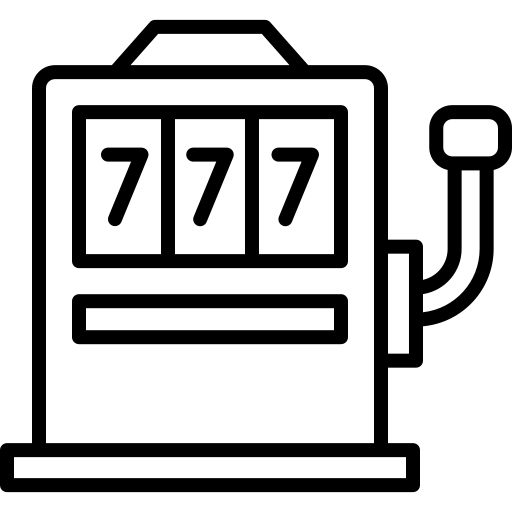
\includegraphics[width=1\linewidth,height=\textheight,keepaspectratio]{lecture3/images/Bandit.png}

\(\Huge{\to}\)

Rewards

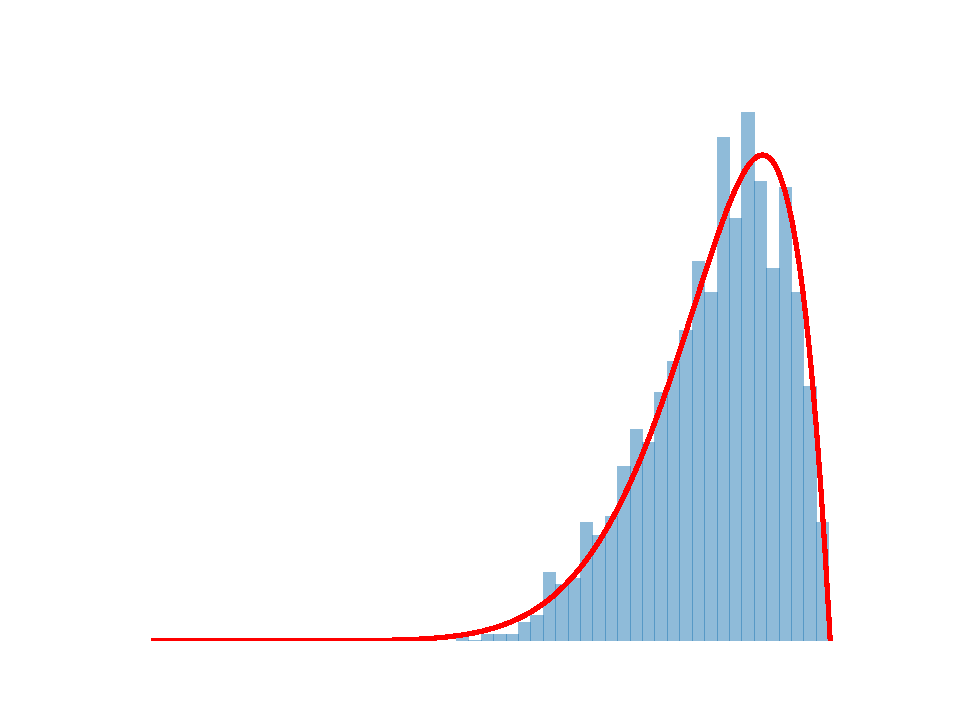
\includegraphics[width=3.125in,height=3.125in]{index_files/mediabag/lecture3/images/Gaussian_1.pdf}

\section{Multi-Armed Bandit}\label{multi-armed-bandit}

\begin{tcolorbox}[enhanced jigsaw, opacityback=0, left=2mm, breakable, bottomtitle=1mm, rightrule=.15mm, colframe=quarto-callout-tip-color-frame, titlerule=0mm, colback=white, opacitybacktitle=0.6, toptitle=1mm, title=\textcolor{quarto-callout-tip-color}{\faLightbulb}\hspace{0.5em}{Nonassociative Environments}, colbacktitle=quarto-callout-tip-color!10!white, bottomrule=.15mm, arc=.35mm, coltitle=black, leftrule=.75mm, toprule=.15mm]

A \emph{nonassociative environment} is a setting that involves learning
how to act in one state. The best example of a nonassociative
environment is Multi-Armed Bandit's.

\end{tcolorbox}

A \textbf{Multi-Armed Bandit} can be interpreted as \emph{k-actions}, or
\emph{k-arms} of the slot machines, to decide from. Through repeated
action selections, you maximize your winnings by concentrating actions
on the best levers.

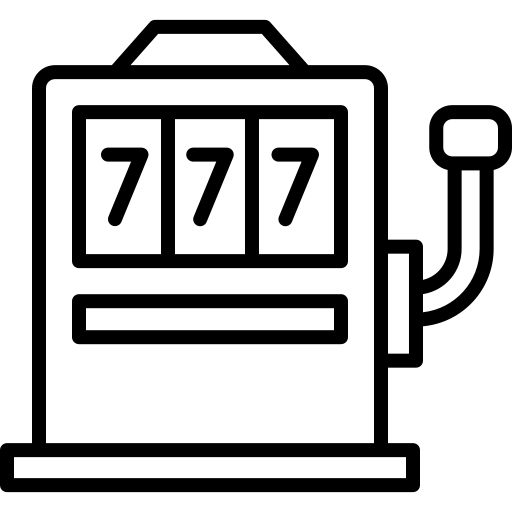
\includegraphics[width=1.82292in,height=1.82292in]{lecture3/images/Bandit.png}\\
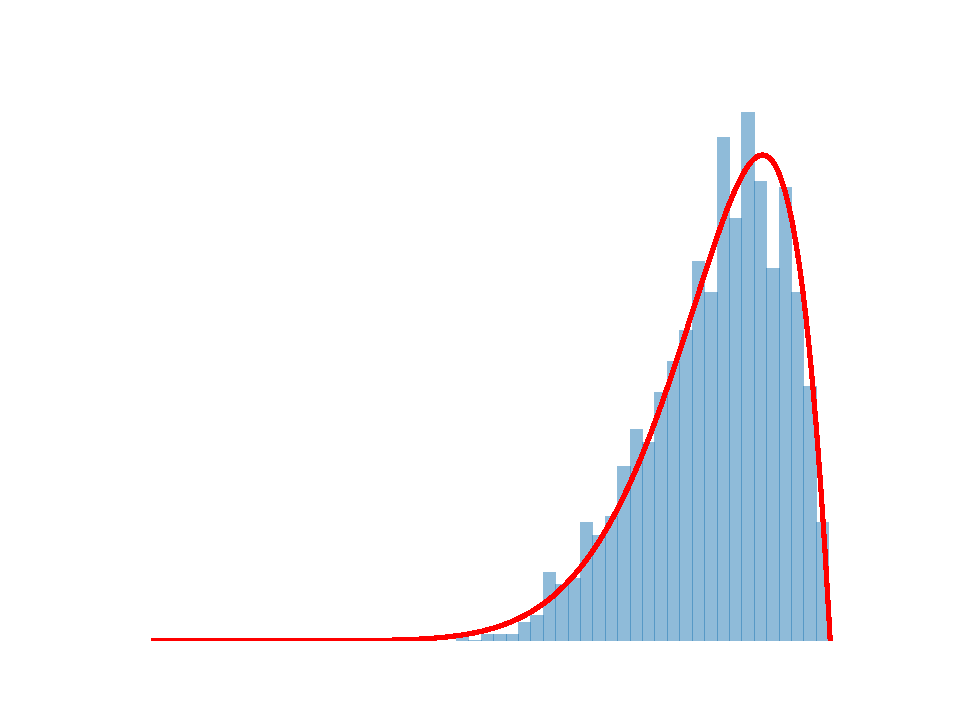
\includegraphics[width=2.08333in,height=2.08333in]{index_files/mediabag/lecture3/images/Gaussian_1.pdf}

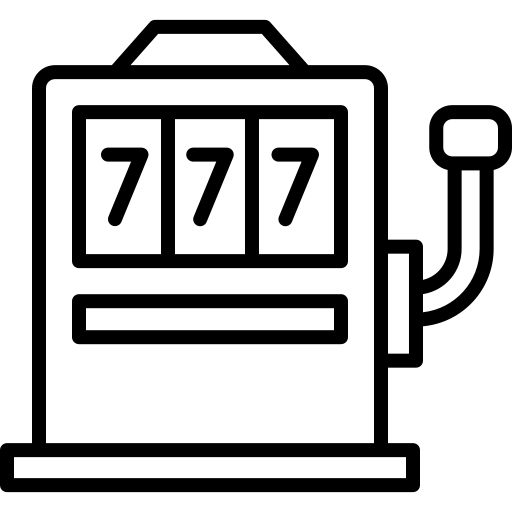
\includegraphics[width=1.82292in,height=1.82292in]{lecture3/images/Bandit.png}\\
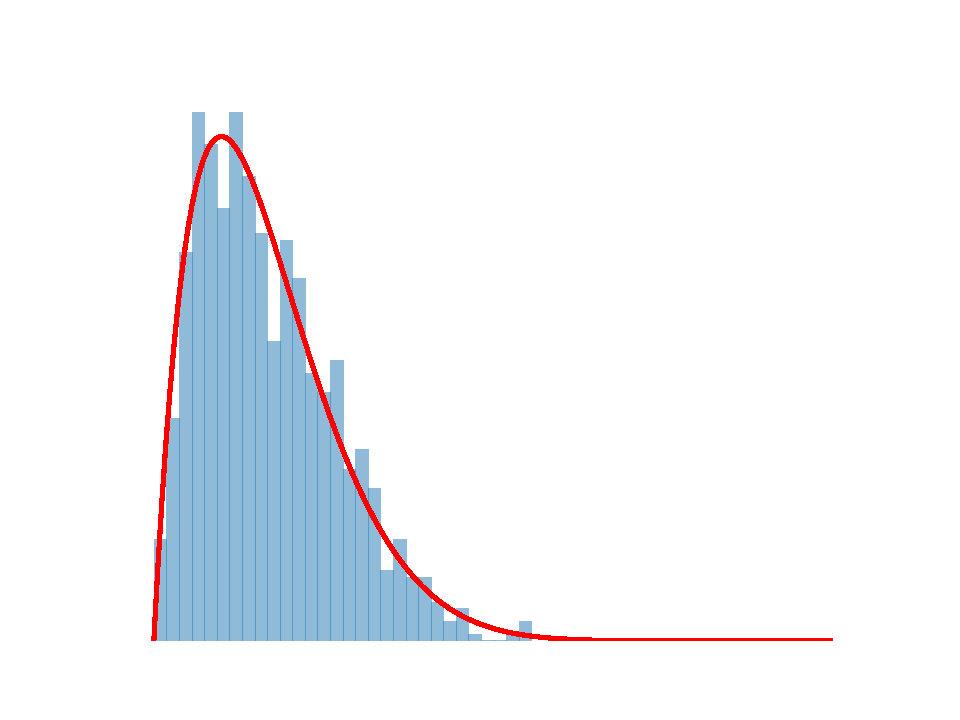
\includegraphics[width=2.08333in,height=2.08333in]{index_files/mediabag/lecture3/images/Gaussian_2.pdf}

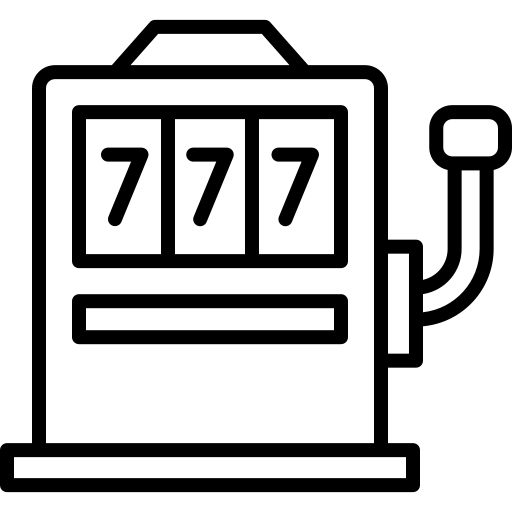
\includegraphics[width=1.82292in,height=1.82292in]{lecture3/images/Bandit.png}\\
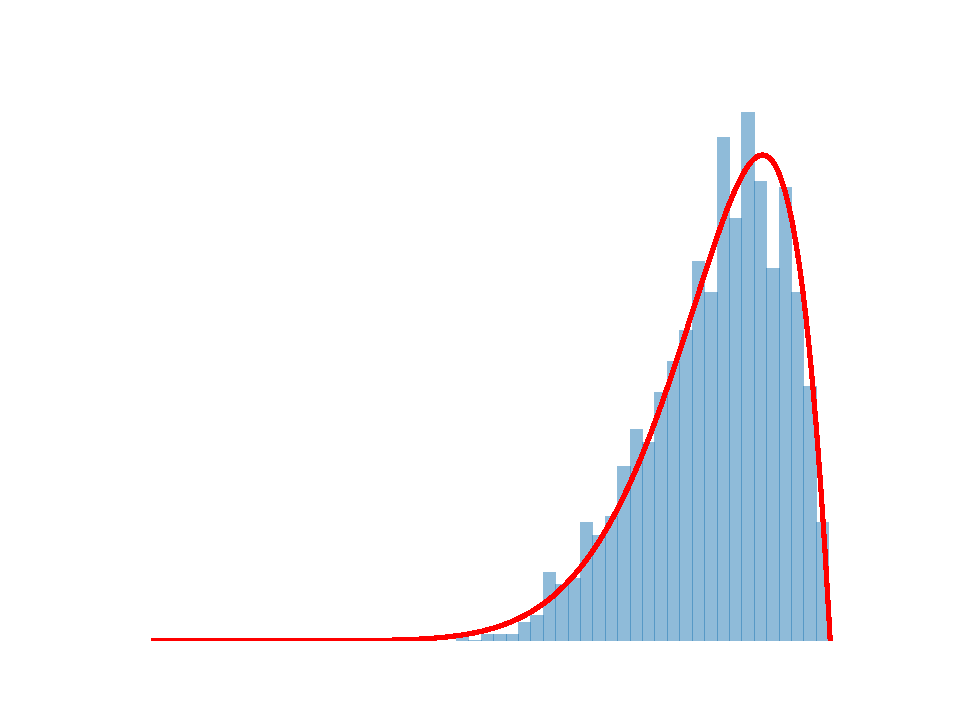
\includegraphics[width=2.08333in,height=2.08333in]{index_files/mediabag/lecture3/images/Gaussian_1.pdf}

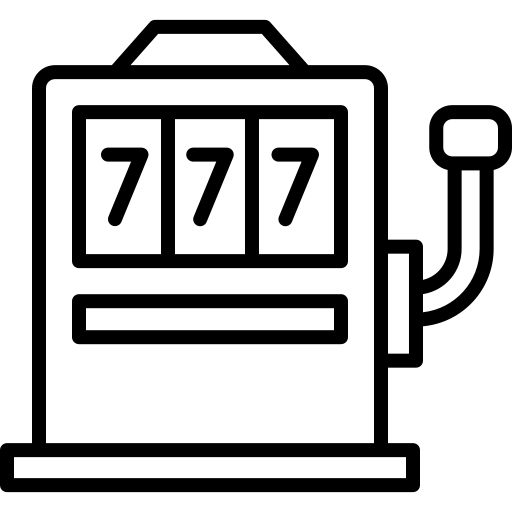
\includegraphics[width=1.82292in,height=1.82292in]{lecture3/images/Bandit.png}\\
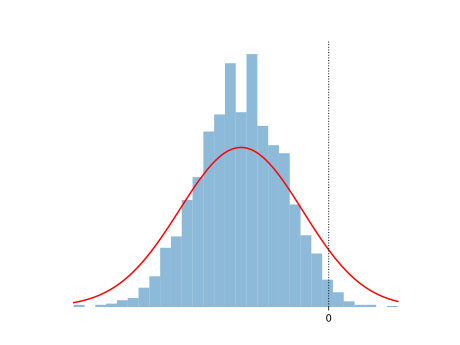
\includegraphics[width=2.08333in,height=2.08333in]{index_files/mediabag/lecture3/images/Gaussian_3.pdf}

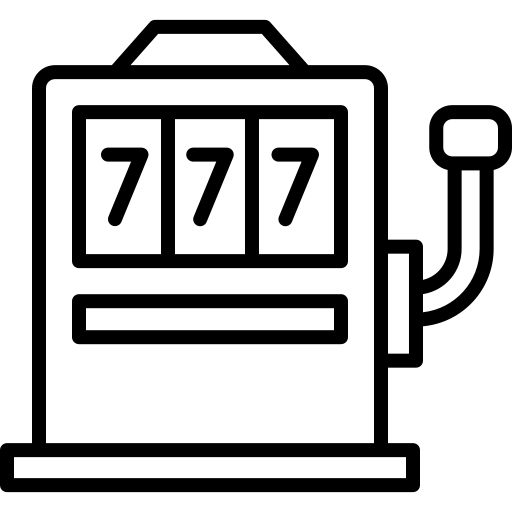
\includegraphics[width=1.82292in,height=1.82292in]{lecture3/images/Bandit.png}\\
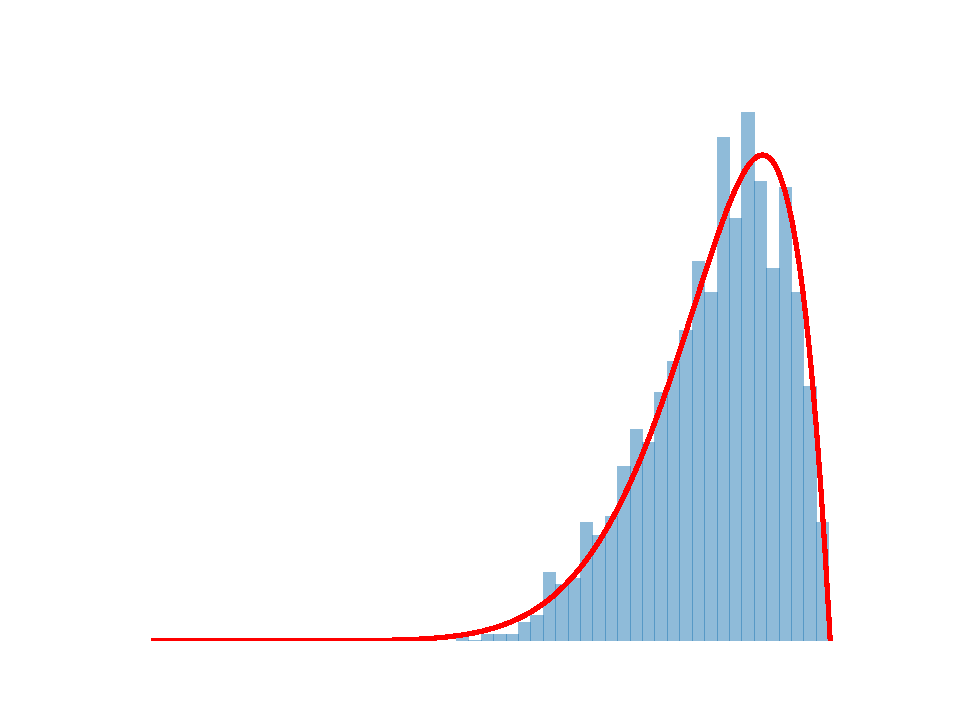
\includegraphics[width=2.08333in,height=2.08333in]{index_files/mediabag/lecture3/images/Gaussian_1.pdf}

\begin{tcolorbox}[enhanced jigsaw, colback=white, left=2mm, breakable, opacityback=0, bottomrule=.15mm, rightrule=.15mm, arc=.35mm, colframe=quarto-callout-note-color-frame, leftrule=.75mm, toprule=.15mm]

How do we decide the most appropriate action? 🤔

\end{tcolorbox}

\section{Expectation of a Bandit}\label{expectation-of-a-bandit}

Each bandit has an expected reward given a particular action is
selected, called the \textbf{action value}.

\[
Q_t(a) = \mathbb{E}[R_t | A_t = a]
\]

Where:

\begin{itemize}
\tightlist
\item
  \(Q_t(a)\) is the \emph{conditional expectation} of the rewards
  \(R_t\) given the selection of an action \(A_t\).
\item
  \(R_t\) is the \emph{random variable} for the reward at time step
  \(t\).
\item
  \(A_t\) is the \emph{random variable} for the action selected at time
  step \(t\).
\end{itemize}

\section{Action Value Method}\label{action-value-method}

To compute expectations of action values and select actions, we use
\textbf{action value methods}.

\[
Q_t(a) = \frac{\sum_{i=1}^{t-1} R_i * \mathbf{1}_{A_i = a}}{\sum_{i=1}^{t-1} \mathbf{1}_{A_i = a}}
\]

Where:

\begin{itemize}
\tightlist
\item
  \(Q_t(a)\) is the action value for a particular action \(a\).
\item
  \(\mathbf{1}\) is a predicate, which denotes whether \(A_i = a\) is
  true or false.
\end{itemize}

If the denominator is \(0\), then we denote \(Q_t(a)\) as \(0\).

\section{Action Value Method Update}\label{action-value-method-update}

To avoid computationally expensive updates using the predicate method,
we can update action values in an incremental fashion:

\[
Q_{t+1} = Q_t + \frac{1}{t} (R_t - Q_t)
\]

or

\[
NewEstimate \gets OldEstimate + StepSize [Target - OldEstimate]
\]

\begin{tcolorbox}[enhanced jigsaw, colback=white, left=2mm, breakable, opacityback=0, bottomrule=.15mm, rightrule=.15mm, arc=.35mm, colframe=quarto-callout-note-color-frame, leftrule=.75mm, toprule=.15mm]

Should we always pick actions with the highest expected value? 🤔

\end{tcolorbox}

\chapter{3.2 ε-Greedy}\label{ux3b5-greedy}

\begin{tcolorbox}[enhanced jigsaw, colback=white, left=2mm, breakable, opacityback=0, bottomrule=.15mm, rightrule=.15mm, arc=.35mm, colframe=quarto-callout-note-color-frame, leftrule=.75mm, toprule=.15mm]

A formal framework that defines probability using three fundamental
rules, ensuring consistency in measuring uncertainty. 🎲

\end{tcolorbox}

\section{Exploring vs.~Exploiting}\label{exploring-vs.-exploiting}

\begin{itemize}
\tightlist
\item
  We are \textbf{exploring} when we randomly select an action.
\end{itemize}

Intuition: \emph{Acting randomly.}

\begin{itemize}
\tightlist
\item
  We are \textbf{exploiting} when an action is selected based on its
  expected value. When we act this way, we are said to be acting in a
  \emph{greedy} manner.
\end{itemize}

Intuition: \emph{Acting systematically.}

\section{Conflict of Exploring
vs.~Exploiting}\label{conflict-of-exploring-vs.-exploiting}

\begin{itemize}
\item
  \textbf{Exploring all of the time} does not permit you to exploit your
  knowledge of expected values.
\item
  \textbf{Exploiting all of the time} does not permit you to explore all
  of the options.
\end{itemize}

Thus, our decision-making must encompass a balance of exploring and
exploiting actions.

\section{The Role of ε}\label{the-role-of-ux3b5}

Epsilon (\(\epsilon\)) is a fixed proportion that decides whether we
explore or exploit our actions. \[
  A_t \gets 
  \begin{cases}
      \text{a random action with probability } \epsilon \\
      \arg\max_a Q(a) \text{ with probability } 1 - \epsilon
  \end{cases}
\]

Hence, \textbf{Epsilon Greedy} is an algorithm that allows us to balance
our decision-making in this simple manner.

\subsection{Pseudocode}\label{pseudocode}

\begin{algorithm}[htb!]
\caption{MAB $\epsilon$-Greedy}
\begin{algorithmic}[1]
\State Initialize, for $a = 1$ to $k$:
\State $Q(a) \gets 0$ 
\State $N(a) \gets 0$ \\
\For{$t$ in range($len(data)$)}
    \State $A_t \gets
        \begin{cases}
            \text{a random action with probability } \epsilon \\
            \text{argmax}_a\, Q(a) \text{ with probability } 1-\epsilon 
        \end{cases}$
    \State $R_t \gets \text{bandit}(A_t)$
    \State $N(A_t) \gets N(A_t) + 1$
    \State $Q(A_t) \gets Q(A_t) + \frac{1}{N(A_t)}[R_t - Q(A_t)]$
\Endfor

\end{algorithmic}
\end{algorithm}

\chapter{3.3 Upper Confidence Boundary
(UCB)}\label{upper-confidence-boundary-ucb}

\begin{tcolorbox}[enhanced jigsaw, colback=white, left=2mm, breakable, opacityback=0, bottomrule=.15mm, rightrule=.15mm, arc=.35mm, colframe=quarto-callout-note-color-frame, leftrule=.75mm, toprule=.15mm]

A formal framework that defines probability using three fundamental
rules, ensuring consistency in measuring uncertainty. 🎲

\end{tcolorbox}

\section{Upper Confidence Boundaries}\label{upper-confidence-boundaries}

\textbf{Upper Confidence Boundaries} allow us to select among the
non-greedy actions according to their potential for actually being
optimal.

\[
A_t \gets \arg\max_a \left[ Q(a) + \sqrt{\frac{2 \ln(t)}{N(a)}} \right]
\]

Where:

\begin{itemize}
\tightlist
\item
  \(\sqrt{\frac{2 \ln(t)}{N(a)}}\) is the measure of variance of the
  action \(a\).
\item
  The natural logarithm increases get smaller over time but are
  unbounded, so all actions will be selected.
\end{itemize}

\section{UCB Exploring
vs.~Exploiting}\label{ucb-exploring-vs.-exploiting}

Each time \(a\) is selected, the uncertainty is presumably reduced:
\(N(a)\) increments, and as it appears in the denominator, the
uncertainty term decreases.

\[
VAR \downarrow = \sqrt{\frac{2 \ln(t)}{N(a)\uparrow}}
\]

Each time an action other than \(a\) is selected, \(t\) increases but
\(N(a)\) does not; because \(t\) appears in the numerator, the
uncertainty estimate increases.

\[
VAR \uparrow = \sqrt{\frac{2 \ln(t) \uparrow}{N(a)}}
\]

\subsection{Pseudocode}\label{pseudocode-1}

\begin{algorithm}[htb!]
\caption{MAB Upper Confidence Boundary (UCB)}
\begin{algorithmic}[1]
\State Initialize, for $a = 1$ to $k$:
\State $Q(a) \gets 0$ 
\State $N(a) \gets 0$ \\
\For{$t$ in range($len(data)$)}
    \State $A_t \gets argmax_a[Q(a) + \sqrt{(\frac{2 ln(t)}{N(a)})}]$
    \State $R_t \gets \text{bandit}(A_t)$
    \State $N(A_t) \gets N(A_t) + 1$
    \State $Q(A_t) \gets Q(A_t) + \frac{1}{N(A_t)}[R_t - Q(A_t)]$
\Endfor

\end{algorithmic}
\end{algorithm}

\chapter{3.4 Thompson Sampling}\label{thompson-sampling}

\begin{tcolorbox}[enhanced jigsaw, colback=white, left=2mm, breakable, opacityback=0, bottomrule=.15mm, rightrule=.15mm, arc=.35mm, colframe=quarto-callout-note-color-frame, leftrule=.75mm, toprule=.15mm]

A formal framework that defines probability using three fundamental
rules, ensuring consistency in measuring uncertainty. 🎲

\end{tcolorbox}

\section{Beta Distribution}\label{beta-distribution-1}

\textbf{Thompson sampling} is an algorithm that leverages the beta
distribution for its action value method and action selections.

Initialize beta distributed with parameters:

\[
\alpha(a) = (\alpha_{1}, . . . , \alpha_{k}) = 1
\] \[
\beta(a) = (\beta_{1}, . . . , \beta_{k}) = 1
\]

Now for each action \(a\), the prior probability density function of our
action value method \(Q(a)\) is:

\[
  Q(a) = \frac{\Gamma(\alpha(a) + \beta(a))}{\Gamma(\alpha(a)) \ \Gamma(\beta(a))} a^{\alpha(a)-1} (1 a)^{\beta(a)-1}
\]

\section{Thompson Sampling Exploring
vs.~Exploiting}\label{thompson-sampling-exploring-vs.-exploiting}

The agent updates its prior belief using the following action value
method:

\[
\alpha(A_{t}) \gets \alpha(A_{t}) + R_{t}
\] \[
\beta(A_{t}) \gets \beta(A_{t}) + 1 R_{t}
\]

Notice that for those actions selected \(A_t\), we increase its
corresponding \(\alpha\) parameter (\(R_t = 1\)) and maintain its
\(\beta\) parameter the same as before (\(1 - R_t = 1 - 1 = 0\)).

This update allows the algorithm to draw accurate samples and strike a
balance between exploring and exploiting.

\subsection{Pseudocode}\label{pseudocode-2}

\begin{algorithm}[htb!]
\caption{MAB Thompson Sampling}
\begin{algorithmic}[1]
\State Initialize, for $a = 1$ to $k$:
\State $\alpha(a) \gets 1$ 
\State $\beta(a) \gets 1$ \\
\For{$t$ in range($len(data)$)}
    \State $Q(a) \leftarrow beta(\alpha(a),\beta(a))$
    \State $A_t \leftarrow argmax_a Q(a)$
    \State $R_t \gets \text{bandit}(A_t)$
    \State $\alpha(A_t) \leftarrow \alpha(A_t) + R_t$
    \State $\beta(A_t) \leftarrow \beta(A_t) + 1 - R_t$
\Endfor
\end{algorithmic}
\end{algorithm}

\part{Lecture 4: Dynamic Programming}

\chapter{Learning Objectives}\label{learning-objectives-2}

\begin{tcolorbox}[enhanced jigsaw, colback=white, left=2mm, breakable, opacityback=0, bottomrule=.15mm, rightrule=.15mm, arc=.35mm, colframe=quarto-callout-note-color-frame, leftrule=.75mm, toprule=.15mm]

Learning Objectives for Lecture 4: Dynamic Programming 🎯

\end{tcolorbox}

\begin{itemize}
\tightlist
\item
  Markov Chain.
\item
  Markov Decision Process (MDPs).
\item
  Dynamic Programming.
\item
  Homemade GridWorld OpenAI environment using \texttt{gymnasium},
  \texttt{pygame} \& \texttt{numpy}.
\end{itemize}

\begin{figure}[H]

{\centering \pandocbounded{\includegraphics[keepaspectratio]{index_files/mediabag/lecture4/images/Lecture4.drawio.pdf}}

}

\caption{Taxonomy of Reinforcement Learning}

\end{figure}%

\chapter{4.1 Markov Chain}\label{markov-chain}

\begin{tcolorbox}[enhanced jigsaw, colback=white, left=2mm, breakable, opacityback=0, bottomrule=.15mm, rightrule=.15mm, arc=.35mm, colframe=quarto-callout-note-color-frame, leftrule=.75mm, toprule=.15mm]

A formal framework that defines probability using three fundamental
rules, ensuring consistency in measuring uncertainty. 🎲

\end{tcolorbox}

\begin{tcolorbox}[enhanced jigsaw, opacityback=0, left=2mm, breakable, bottomtitle=1mm, rightrule=.15mm, colframe=quarto-callout-tip-color-frame, titlerule=0mm, colback=white, opacitybacktitle=0.6, toptitle=1mm, title=\textcolor{quarto-callout-tip-color}{\faLightbulb}\hspace{0.5em}{Associative Environments}, colbacktitle=quarto-callout-tip-color!10!white, bottomrule=.15mm, arc=.35mm, coltitle=black, leftrule=.75mm, toprule=.15mm]

A \emph{associative environment} is a setting that involves learning how
to act in multiple states. The best frameworks to generalize associative
environments are Markov models.

\end{tcolorbox}

\section{Markov Models}\label{markov-models}

All Markov models assume the \textbf{Markov Property}, meaning that
\emph{future states depend only on current states and not previous
states}.

\[
P(s’ | s, s_{t-1}, s_{t-2}, \dots) = P(s’ | s)
\]

Markov models differ based on whether every sequential state is
observable and whether the system is adjusted based on observations:

\begin{longtable}[]{@{}
  >{\raggedright\arraybackslash}p{(\linewidth - 4\tabcolsep) * \real{0.3333}}
  >{\raggedright\arraybackslash}p{(\linewidth - 4\tabcolsep) * \real{0.3333}}
  >{\raggedright\arraybackslash}p{(\linewidth - 4\tabcolsep) * \real{0.3333}}@{}}
\toprule\noalign{}
\begin{minipage}[b]{\linewidth}\raggedright
\end{minipage} & \begin{minipage}[b]{\linewidth}\raggedright
States are fully observable
\end{minipage} & \begin{minipage}[b]{\linewidth}\raggedright
States are partially observable
\end{minipage} \\
\midrule\noalign{}
\endhead
\bottomrule\noalign{}
\endlastfoot
Decision-making is not controlled & \textbf{Markov Chain} & Hidden
Markov Model \\
Decision-making is controlled & \textbf{Markov Decision Process} &
Partially Observable Markov Decision Process \\
\end{longtable}

\section{Markov Chain}\label{markov-chain-1}

A \textbf{Markov Chain} is a model for transitions that are \emph{not
controlled} between \emph{fully observable states}. A \textbf{State} is
a node. A \textbf{State Transition} is one outward-going arrow. State
transitions are conditional probabilities of going to the next state
given the current state.

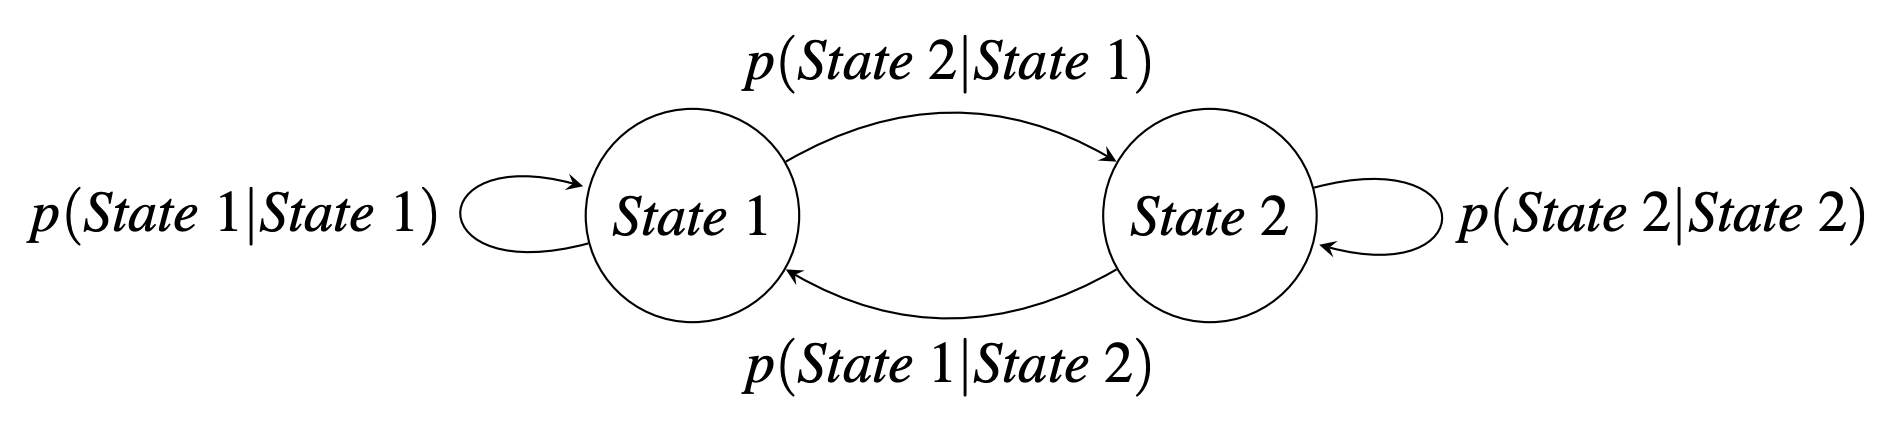
\includegraphics[width=0.75\linewidth,height=\textheight,keepaspectratio]{lecture4/images/markovchain-ex.png}

\section{Probability Matrix}\label{probability-matrix}

Suppose a frog jumps from one lily pad to another with state transition
probabilities:

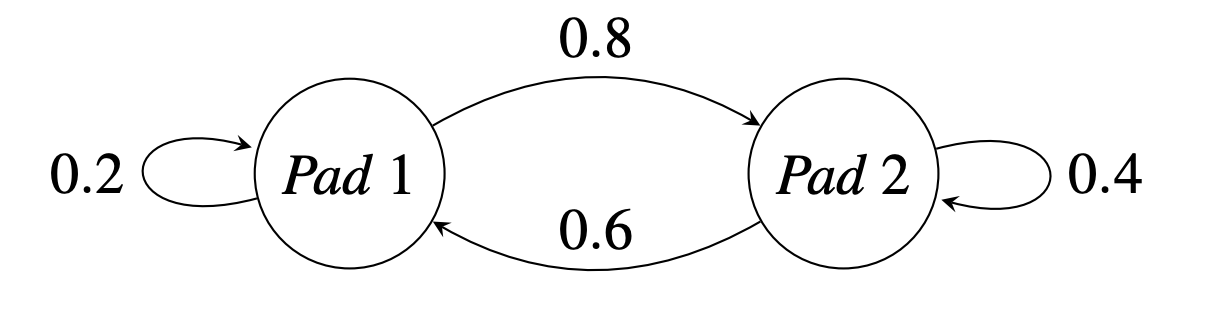
\includegraphics[width=0.5\linewidth,height=\textheight,keepaspectratio]{lecture4/images/markovchain-ex-prob.png}

\[
\mathbf{P} = \begin{bmatrix} 0.2 & 0.6 \\ 0.8 & 0.4 \end{bmatrix}
\]

\section{Rewards Matrix}\label{rewards-matrix}

Suppose the frog has associated rewards:

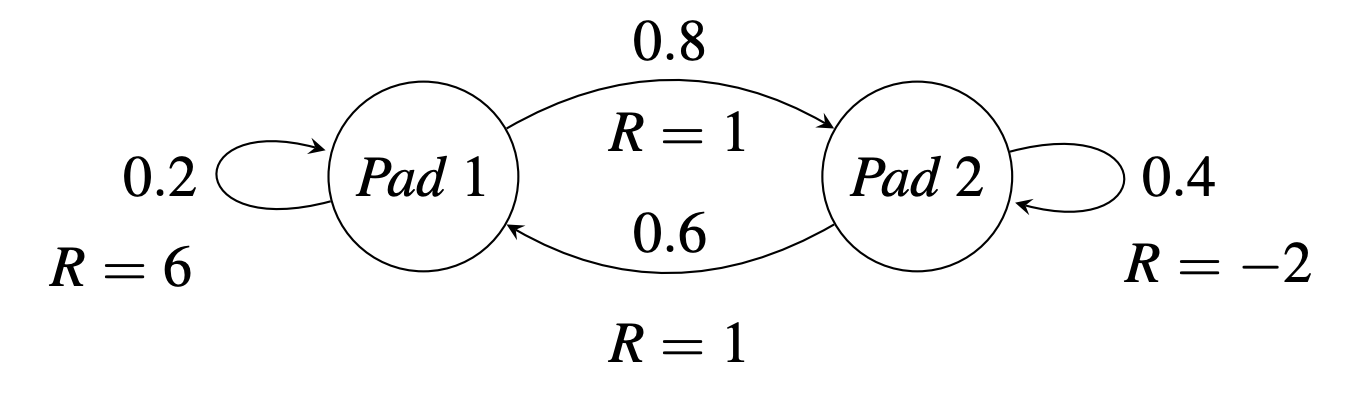
\includegraphics[width=0.5\linewidth,height=\textheight,keepaspectratio]{lecture4/images/markovchain-ex-prob-rew.png}

\[
\mathbf{R} = \begin{bmatrix} 6 & 1 \\ 1 & -2 \end{bmatrix}
\]

\section{Value Function}\label{value-function}

We want to calculate the expected value of moving from state \(i\) to
state \(j\) for all situations \(s \in \{1,2,...,S\}\):

\[
\begin{align*}
v_{j}(t) & = \sum_{i=1}^{S} p_{i,j} \ [r_{i,j}+v_{i}(t-1)] \\
& = \sum_{i=1}^{S} p_{i,j} \ r_{i,j} + \sum_{i=1}^{S} p_{i,j} \ v_{i}(t-1) \\ 
& = \textbf{q} + \sum_{i=1}^{S} p_{i,j}\ v_{i}(t-1)
\end{align*}
\]

\[
\mathbf{v}(t) = \mathbf{q} + \mathbf{v}(t-1) \mathbf{P}
\]

First, we need to calculate \(\textbf{q}\), the expected reward in the
next transition out of state \(i\):

\[
\mathbf{q} = \sum_{i=1}^{S} p_{i,j} r_{i,j}
\]

\[
q_{1} = p_{1,1} \ r_{1,1} + r_{2,1} \ p_{2,1}
\]

\[
q_{2} = p_{1,2} \ r_{1,2} + r_{2,2} \ p_{2,2}
\]

\[
\textbf{q} = 
\begin{bmatrix}
    2 & -0.2
\end{bmatrix}
\]

\[
\begin{bmatrix} v_{1}(t) \ v_{2}(t) \end{bmatrix} = \begin{bmatrix} 2 \ -0.2 \end{bmatrix} + \begin{bmatrix} v_{1}(t-1) \ v_{2}(t-1) \end{bmatrix} \begin{bmatrix} 0.2 & 0.6 \\ 0.8 & 0.4 \end{bmatrix}
\]

At \(t=100\): \[
\mathbf{v}(100) = \begin{bmatrix} 77.88 & 76.59 \end{bmatrix}
\]

In other words, the frogs expected value at \(t = 100\) is that lilly
pad \(1\) will be greater (with \(77.88\) expected flies) than that of
lilly pad \(2\) (with \(76.59\) expected flies)

\section{Asymptotic Behavior}\label{asymptotic-behavior}

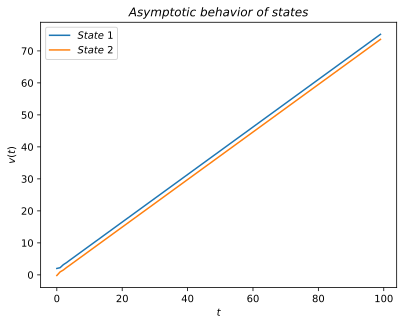
\includegraphics[width=0.5\linewidth,height=\textheight,keepaspectratio]{index_files/mediabag/lecture4/images/MCAsymptotic_.pdf}

\section{Discounting Factor}\label{discounting-factor}

\item

The \textbf{Discounting Factor} \(\gamma\) allows us to place a higher
value on the present rewards, rather than future uncertain rewards.

\[
\mathbf{v}(t) = \mathbf{q} + \gamma \mathbf{v}(t-1) \mathbf{P}
\]

\[
\begin{bmatrix} v_{1}(t) \ v_{2}(t) \end{bmatrix} = \begin{bmatrix} 2 \ -0.2 \end{bmatrix} + \gamma \begin{bmatrix} v_{1}(t-1) \ v_{2}(t-1) \end{bmatrix} \begin{bmatrix} 0.2 & 0.6 \\ 0.8 & 0.4 \end{bmatrix}
\]

At \(\gamma=0.9\) and \(t=100\): \[
\mathbf{v}(100) = \begin{bmatrix} 8.47 & 7.15 \end{bmatrix}
\]

\section{Discounted Asymptotic
Behavior}\label{discounted-asymptotic-behavior}

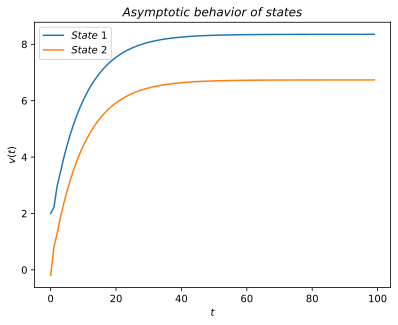
\includegraphics[width=0.5\linewidth,height=\textheight,keepaspectratio]{index_files/mediabag/lecture4/images/MCAsymptotic.pdf}

\chapter{Python Code}\label{python-code}

\begin{Shaded}
\begin{Highlighting}[]
\ImportTok{import}\NormalTok{ numpy }\ImportTok{as}\NormalTok{ np}

\NormalTok{GAMMA }\OperatorTok{=} \FloatTok{0.9}
\NormalTok{P }\OperatorTok{=}\NormalTok{ np.array([[}\FloatTok{0.2}\NormalTok{, }\FloatTok{0.6}\NormalTok{], [}\FloatTok{0.8}\NormalTok{, }\FloatTok{0.4}\NormalTok{]])}
\NormalTok{R }\OperatorTok{=}\NormalTok{ np.array([[}\DecValTok{6}\NormalTok{, }\DecValTok{1}\NormalTok{], [}\DecValTok{1}\NormalTok{, }\OperatorTok{{-}}\DecValTok{2}\NormalTok{]])}
\NormalTok{q }\OperatorTok{=}\NormalTok{ np.}\BuiltInTok{sum}\NormalTok{(P }\OperatorTok{*}\NormalTok{ R, axis}\OperatorTok{=}\DecValTok{1}\NormalTok{)}
\NormalTok{v\_initial }\OperatorTok{=}\NormalTok{ np.array([}\DecValTok{0}\NormalTok{, }\DecValTok{0}\NormalTok{])}

\KeywordTok{def}\NormalTok{ value\_function(v, P, q, t}\OperatorTok{=}\DecValTok{100}\NormalTok{):}
    \ControlFlowTok{for}\NormalTok{ \_ }\KeywordTok{in} \BuiltInTok{range}\NormalTok{(t):}
\NormalTok{        v }\OperatorTok{=}\NormalTok{ q }\OperatorTok{+}\NormalTok{ GAMMA }\OperatorTok{*}\NormalTok{ np.dot(v, P)}
    \ControlFlowTok{return}\NormalTok{ v}

\NormalTok{v\_result }\OperatorTok{=}\NormalTok{ value\_function(v\_initial, P, q)}
\BuiltInTok{print}\NormalTok{(v\_result)}
\end{Highlighting}
\end{Shaded}

\chapter{4.2 Markov Decision Process
(MDPs)}\label{markov-decision-process-mdps}

\begin{tcolorbox}[enhanced jigsaw, colback=white, left=2mm, breakable, opacityback=0, bottomrule=.15mm, rightrule=.15mm, arc=.35mm, colframe=quarto-callout-note-color-frame, leftrule=.75mm, toprule=.15mm]

A formal framework that defines probability using three fundamental
rules, ensuring consistency in measuring uncertainty. 🎲

\end{tcolorbox}

\section{Markov Decision Process}\label{markov-decision-process}

A \textbf{Markov Decision Process} (MDP) is a model for transitions that
are \emph{controlled} between \emph{fully observable states}. The
\textbf{Agent} is the learner and decision-maker. The
\textbf{Environment} is everything external to the agent. From an
\textbf{Initial State}, the agent interacts with the environment through
its \textbf{Actions}. These actions continuously give rise to different
\textbf{States} and \textbf{Rewards}.

\begin{center}
\includegraphics[width=0.75\linewidth,height=\textheight,keepaspectratio]{lecture4/images/MDP.png}
\end{center}

\subsection{Environment GridWorld}\label{environment-gridworld}

\begin{center}
\includegraphics[width=0.65\linewidth,height=\textheight,keepaspectratio]{lecture4/images/MDPGridworld-ex.png}
\end{center}

\begin{itemize}
\tightlist
\item
  Actions are equally likely to occur.
\item
  Actions that take the agent out of the environment receive a reward of
  \(-1\), actions that take the agent to the terminal state (shaded in
  gray) receive a reward of \(+1\), and all other actions receive a
  reward of \(0\).
\item
  Our objective is to calculate the shortest path from any state to the
  optimal state.
\end{itemize}

\section{Sequential Interaction}\label{sequential-interaction}

For a finite discrete number of time steps \(t = 0, 1, 2, 3...,T\)
(where \(T\) is the terminal time step marking the end of an episode)
the \textbf{sequential interaction} is:

\begin{enumerate}
\def\labelenumi{\arabic{enumi}.}
\tightlist
\item
  The agent receives an interpretation from the state \(s_t \in S\).
\item
  The agent makes an action \(a_t \in A(s_t)\) based on the situation.
\item
  The agent receives a reward \(r_{t+1} \in R \subseteq \mathbb{R}\)
  from its environment and finds itself in a new state \(s_{t+1}\) based
  on the action taken.
\end{enumerate}

The sequence continues in the form:

\[
s_0, a_0, r_1, s_1, a_1, r_2, s_2, a_2, r_3,...
\]

\subsection{Environment GridWorld}\label{environment-gridworld-1}

Sequential interaction for one episode:

\begin{center}
\includegraphics[width=0.75\linewidth,height=\textheight,keepaspectratio]{lecture4/images/SequentialGridworld-ex.png}
\end{center}

Notice that, for now, state transitions are \textbf{deterministic}. In
other words, we assume a perfect model of the environment. We do not
care about \textbf{stochastic} state transitions (this is something that
we will visit in the next lectures).

\section{Policy}\label{policy}

A \textbf{Policy} is a mapping from states to probabilities of selecting
each possible action, denoted as:

\[
\pi(a|s)
\]

\begin{center}
\includegraphics[width=0.35\linewidth,height=\textheight,keepaspectratio]{lecture4/images/Policy.png}
\end{center}

\[
\sum_{a \in A(s)} \pi(a|s) = 1 \quad \text{for all } s \in S
\]

\subsection{Environment GridWorld}\label{environment-gridworld-2}

\begin{center}
\includegraphics[width=0.55\linewidth,height=\textheight,keepaspectratio]{lecture4/images/GridWorld-Policy.png}
\end{center}

Since all actions are equally likely, we are said to be following a
\textbf{random policy}:

\[
\pi(a_0|s_0) = \frac{1}{4}
\]

\section{Dynamic Function}\label{dynamic-function}

The \textbf{dynamic function} is a mapping of the state transition
probabilities of the MDP for each possible reward:

\[
p(s^{'}, r | s, a)
\]

\begin{center}
\includegraphics[width=0.35\linewidth,height=\textheight,keepaspectratio]{lecture4/images/DynamicFunction.png}
\end{center}

As mentioned before, the dynamics of GridWorld are
\textbf{deterministic} leading to the same new state given each state
and action:

\[
\sum_{s^{'} \in S}\sum_{r \in R} p(s^{'}, r| s, a) = 1 \quad \text{for all } s \in S \text{ and } a \in A(s)
\]

\subsection{Environment GridWorld}\label{environment-gridworld-3}

\begin{center}
\includegraphics[width=0.55\linewidth,height=\textheight,keepaspectratio]{lecture4/images/GridWorldDynamicFunction.png}
\end{center}

As mentioned before, the dynamics of GridWorld are
\textbf{deterministic}, leading to the same new state given each state
and action:

\[
p(s_{1}, r_{1}| s_0, a_{0}) = 1
\]

\section{Goal}\label{goal}

Our \textbf{Goal} \(G_{t}\) is to maximize the expected return of the
discounted reward sequence:

\[
\begin{aligned}
G_{t} = r_{t+1} + \gamma r_{t+2} + \ldots + \gamma^{T-1} r_{T} \\
     = r_{t+1} + \gamma (r_{t+2} + \ldots + \gamma^{T-2} r_{T}) \\
     = r_{t+1} + \gamma G_{t+1} 
\end{aligned}
\]

\subsubsection{Exercise}\label{exercise-8}

Suppose \(\gamma = 0.5\) and the following sequence of rewards is
received \(r_{1} = -1\), \(r_{2} = 2\), \(r_{3} = 6\), \(r_{4} = 3\),
and \(r_{5} = 2\), with \(T = 5\). What are \(G_{0}\), \(G_{1}\),
\ldots, \(G_{5}\)?

\begin{tcolorbox}[enhanced jigsaw, opacityback=0, left=2mm, breakable, bottomtitle=1mm, rightrule=.15mm, colframe=quarto-callout-tip-color-frame, titlerule=0mm, colback=white, opacitybacktitle=0.6, toptitle=1mm, title=\textcolor{quarto-callout-tip-color}{\faLightbulb}\hspace{0.5em}{Solution}, colbacktitle=quarto-callout-tip-color!10!white, bottomrule=.15mm, arc=.35mm, coltitle=black, leftrule=.75mm, toprule=.15mm]

\[
\begin{aligned}
G_{5} &= r_{6} + r_{7} + \dots = 0 \\
G_{4} &= r_{5} + 0.5(G_{5}) = 2 \\
G_{3} &= r_{4} + 0.5(G_{4}) = 4 \\
G_{2} &= r_{3} + 0.5(G_{3}) = 8 \\
G_{1} &= r_{2} + 0.5(G_{2}) = 6 \\
G_{0} &= r_{1} + 0.5(G_{1}) = 2 \\
\end{aligned}
\]

\end{tcolorbox}

\section{Value Functions}\label{value-functions}

\textbf{Value Functions} calculate the expected reward when starting
from the state \(s\) and then interacting with the environment according
to the policy \(\pi\), denoted as:

\[
v_{\pi}(s) = \mathbb{E_{\pi}}[G_{t}| \ s]
\]

\begin{center}
\includegraphics[width=0.35\linewidth,height=\textheight,keepaspectratio]{lecture4/images/ValueFunction.png}
\end{center}

\subsection{Bellman Equation}\label{bellman-equation}

For any policy \(\pi\) and any state \(s\), the Bellman equation holds:

\[
\begin{aligned}
v_{\pi}(s) &= \mathbb{E_{\pi}}[G_{t}| \ s] \\
&= \mathbb{E_{\pi}}[r_{t+1} + \gamma G_{t+1}| \ s] \\
&= \sum_{a} \pi(a|s) \sum_{s^{'},r} p(s^{'},r|s,a)[r_{t+1} + \gamma \mathbb{E_{\pi}}[G_{t+1}| \ s]] \\
&= \underbrace{\sum_{a} \pi(a|s)}_{Policy} \underbrace{\sum_{s^{'}, r} p(s^{'},r|s,a)}_{Dynamic \ Function}\underbrace{[r_{t+1} + \gamma v_{\pi}(s^{'})]}_{Discounted \ Reward \ Sequence}
\end{aligned}
\]

\subsubsection{Exercise}\label{exercise-9}

For the first episode, calculate the value of each state using the
Bellman equation:

\[
v_{\pi}(s) = \sum_{a} \pi(a|s) \sum_{s^{'}, r} p(s^{'},r|s,a)[r + \gamma v_{\pi}(s^{'})]
\]

\begin{center}
\includegraphics[width=0.13\linewidth,height=\textheight,keepaspectratio]{lecture4/images/GridWorldEmpty-ex.png}
\end{center}

\begin{tcolorbox}[enhanced jigsaw, opacityback=0, left=2mm, breakable, bottomtitle=1mm, rightrule=.15mm, colframe=quarto-callout-tip-color-frame, titlerule=0mm, colback=white, opacitybacktitle=0.6, toptitle=1mm, title=\textcolor{quarto-callout-tip-color}{\faLightbulb}\hspace{0.5em}{Solution}, colbacktitle=quarto-callout-tip-color!10!white, bottomrule=.15mm, arc=.35mm, coltitle=black, leftrule=.75mm, toprule=.15mm]

\begin{center}
\includegraphics[width=0.75\linewidth,height=\textheight,keepaspectratio]{lecture4/images/GridWorldSolution.png}
\end{center}

\end{tcolorbox}

\section{Action Value Functions}\label{action-value-functions}

\textbf{Action Value Functions} estimate how good it is for an agent to
follow policy \(\pi\) given the action taken under the previous state:

\[
q_{\pi}(s, a) = \mathbb{E_{\pi}}[G_{t}| \ s, \ a]
\]

\begin{center}
\includegraphics[width=0.35\linewidth,height=\textheight,keepaspectratio]{lecture4/images/ActionValue.png}
\end{center}

\subsection{Bellman Equation}\label{bellman-equation-1}

The action value function is also expressed in terms of the Bellman
equation:

\[
\begin{align}
    q_{\pi}(s, a) & = \mathbb{E_{\pi}}[G_{t}| \ s, \ a] \\
     & = \underbrace{\sum_{s^{'}, r} p(s^{'},r|s,a)}_{Dynamic \ Function} \underbrace{[r + \gamma v_{\pi}(s^{'})]}_{Discounted \ Reward \  Sequence}
\end{align}
\]

Notice that the policy is no longer calculated (since an action has
already taken place according to the policy), and that the quality of
following policy \(\pi\) is calculated in \(v_{\pi}(s^{'})\).

\section{Optimal Policy}\label{optimal-policy}

An \textbf{optimal policy} \(\pi\) is defined to be better than or equal
to a policy \(\pi^{'}\) if its expected return is greater than or equal
to that of \(\pi^{'}\) for all states:

\[
\pi \geq \pi^{'} \quad \text{I.F.F.} \quad v_{\pi} \geq v_{\pi^{'}} \quad \forall s \in S
\]

Since there may be more than one optimal policy, we denote all optimal
policies by \(\pi_{*}\).

\subsection{Optimal Value Function}\label{optimal-value-function}

\[
v_{*}(s) = \max_{a} \sum_{s^{'}, r} p(s^{'},r|s,a) \big[ r + \gamma v_{*}(s^{'}) \big]
\]

\begin{center}
\includegraphics[width=0.35\linewidth,height=\textheight,keepaspectratio]{lecture4/images/OptimValue.png}
\end{center}

\subsection{Optimal Action-Value
Function}\label{optimal-action-value-function}

\[
q_{*}(s, a) = \sum_{s^{'}, r} p(s^{'},r|s,a) \big[ r + \gamma v_{*}(s^{'}) \big]
\]

\begin{center}
\includegraphics[width=0.35\linewidth,height=\textheight,keepaspectratio]{lecture4/images/OptimActionValue.png}
\end{center}

\subsubsection{Exercise}\label{exercise-10}

For the first episode, calculate the optimal value for each state using
the bellman equation:

\[
v_{*}(s) = \max_{a} \sum_{s^{'}, r} p(s^{'},r|s,a) \big[ r + \gamma v_{*}(s^{'}) \big]
\]

\begin{center}
\includegraphics[width=0.13\linewidth,height=\textheight,keepaspectratio]{lecture4/images/GridWorldEmpty-ex.png}
\end{center}

\begin{tcolorbox}[enhanced jigsaw, opacityback=0, left=2mm, breakable, bottomtitle=1mm, rightrule=.15mm, colframe=quarto-callout-tip-color-frame, titlerule=0mm, colback=white, opacitybacktitle=0.6, toptitle=1mm, title=\textcolor{quarto-callout-tip-color}{\faLightbulb}\hspace{0.5em}{Solution}, colbacktitle=quarto-callout-tip-color!10!white, bottomrule=.15mm, arc=.35mm, coltitle=black, leftrule=.75mm, toprule=.15mm]

\begin{center}
\includegraphics[width=0.75\linewidth,height=\textheight,keepaspectratio]{lecture4/images/GridWorldOptimal-sol.png}
\end{center}

Notice the behavior of the optimal policy as \(\pi_{*} \to \infty\)

\begin{center}
\includegraphics[width=0.13\linewidth,height=\textheight,keepaspectratio]{lecture4/images/GridWorldOptim-sol2.png}
\end{center}

\end{tcolorbox}

\chapter{4.3 Dynamic Programming}\label{dynamic-programming}

\begin{tcolorbox}[enhanced jigsaw, colback=white, left=2mm, breakable, opacityback=0, bottomrule=.15mm, rightrule=.15mm, arc=.35mm, colframe=quarto-callout-note-color-frame, leftrule=.75mm, toprule=.15mm]

A formal framework that defines probability using three fundamental
rules, ensuring consistency in measuring uncertainty. 🎲

\end{tcolorbox}

\section{Dynamic Programming}\label{dynamic-programming-1}

\textbf{Dynamic Programming} refers to a collection of algorithms that
can be used to compute optimal policies given a perfect model of the
environment as a Markov decision process (MDP).

These algorithms have limited utility in reinforcement learning due to
their \textbf{assumption of a perfect model} and their
\textbf{computational expense}, but they are still important
theoretically.

In fact, the rest of the course could be seen as a way to replicate the
same effect of dynamic programming without its assumptions.

\subsection{Pseudocode}\label{pseudocode-3}

\begin{algorithm}[htb!]
\caption{Iterative Policy Evaluation (Prediction)}
\begin{algorithmic}[1]  % [1] enables line numbers

\State \textbf{Initialize:} 
\State $V(s) \gets 0$ for all $s \in S$
\State $\gamma \in [0,1)$
\State $\theta \gets 10^{-4}$ \Comment{small positive number for accuracy of estimation}

\Repeat
    \State $\Delta \gets 0$
    \ForAll{$s \in S$}
        \State $v \gets V(s)$
        \State $V(s) \gets \sum_{a} \pi(a|s) \sum_{s',r} p(s',r|s,a) \left[ r + \gamma V(s') \right]$
        \State $\Delta \gets \max(\Delta, |v - V(s)|)$
    \EndFor
\Until{$\Delta < \theta$}

\end{algorithmic}
\end{algorithm}

\section{Policy Improvement}\label{policy-improvement}

We know how good it is to follow the current policy from \(s\) --- that
is \(v_{\pi}(s)\) --- but would it be better or worse to change to a new
policy \(\pi^{'}\)?

One way to check if it is better to switch from policy \(\pi\) to
\(\pi^{'}\) is by checking if the following inequality holds:

\[ 
q_{\pi}(s, \pi^{'}(s)) \geq v_{\pi}(s) 
\]

\emph{Intuition:} If selecting \(a\) in \(s\) and thereafter following
policy \(\pi\) is better than just following \(\pi\), then there must be
a better policy \(\pi^{'}\).

The special case when this inequality is true is referred to as the
\textbf{policy improvement theorem}.

\section{Value Iteration}\label{value-iteration}

One drawback of policy iteration is that policy evaluation is done
iteratively, requiring convergence exactly to \(v_{\pi}\), which occurs
only in the limit.

\textbf{Value Iteration} is a dynamic programming algorithm that
truncates the policy evaluation step after just one sweep.

\subsection{Pseudocode}\label{pseudocode-4}

\begin{algorithm}[htb!]
\caption{Value Iteration}
\begin{algorithmic}[1]
\State \textbf{Initialize:} 
\State $V(s) \gets 0$ for all $s \in S$
\State $\gamma \in [0,1)$
\State $\theta \gets 10^{-4}$  \textit{// small positive number for accuracy of estimation}

\Repeat
    \State $\Delta \gets 0$
    \Forall{$s \in S$}
        \State $v \gets V(s)$
        \State $V(s) \gets \max_a \sum_{s^{'},r} p(s^{'},r|s,a) \left[ r + \gamma V(s^{'}) \right]$
        \State $\Delta \gets \max(\Delta, |v - V(s)|)$
    \Endfor
\Until{$\Delta < \theta$}

\end{algorithmic}
\end{algorithm}

\section{Generalized Policy
Iteration}\label{generalized-policy-iteration}

\textbf{Generalized Policy Iteration} refers to the general idea of
letting policy evaluation and policy improvement processes interact,
regardless of anything else.

Almost all of RL can be described as the policy always being improved
with respect to the value function, and the value function always being
driven toward the value function for the policy.

\begin{center}
\includegraphics[width=0.4\linewidth,height=\textheight,keepaspectratio]{lecture4/images/GPI.png}
\end{center}

\part{Lecture 5: Monte Carlo}

\chapter{Learning Objectives}\label{learning-objectives-3}

\begin{tcolorbox}[enhanced jigsaw, colback=white, left=2mm, breakable, opacityback=0, bottomrule=.15mm, rightrule=.15mm, arc=.35mm, colframe=quarto-callout-note-color-frame, leftrule=.75mm, toprule=.15mm]

Learning Objectives for Lecture 5: Monte Carlo 🎯

\end{tcolorbox}

\begin{itemize}
\tightlist
\item
  Monte Carlo Prediction.
\item
  On-Policy Monte Carlo.
\item
  Off-Policy Monte Carlo.
\item
  Homemade GridWorld OpenAI environment using \texttt{gymnasium},
  \texttt{pygame} \& \texttt{numpy}.
\end{itemize}

\begin{figure}[H]

{\centering \pandocbounded{\includegraphics[keepaspectratio]{index_files/mediabag/lecture5/images/Lecture5.drawio.pdf}}

}

\caption{Taxonomy of Reinforcement Learning}

\end{figure}%

\chapter{5.1 Monte Carlo Prediction}\label{monte-carlo-prediction}

\begin{tcolorbox}[enhanced jigsaw, colback=white, left=2mm, breakable, opacityback=0, bottomrule=.15mm, rightrule=.15mm, arc=.35mm, colframe=quarto-callout-note-color-frame, leftrule=.75mm, toprule=.15mm]

A formal framework that defines probability using three fundamental
rules, ensuring consistency in measuring uncertainty. 🎲

\end{tcolorbox}

\section{Monte Carlo}\label{monte-carlo}

\textbf{Monte Carlo} is a powerful \emph{learning rule} for estimating
value functions \(v_{\pi}\) and action value functions \(q_{\pi}\) in
associative environments.

The power of Monte Carlo resides in its ability to \emph{learn the
dynamics of any environment, without assuming any prior knowledge, only
using experience}.

\section{Monte Carlo Prediction}\label{monte-carlo-prediction-1}

Monte Carlo methods are based on averaging sample returns of
trajectories following a policy \(\pi\).

Recall that returns are calculated as follows:

\[ 
G_{t} = r_{t+1} + \gamma G_{t+1} 
\]

Only on the completion of an episode are value estimates \(v_{\pi}(s)\)
and action value estimates \(q_{\pi}(s,a)\) updated.

\begin{center}
\includegraphics[width=0.1\linewidth,height=\textheight,keepaspectratio]{lecture5/images/MonteCarlo.png}
\end{center}

\subsection{Pseudocode}\label{pseudocode-5}

\begin{algorithm}[htb!]
\caption{Monte Carlo Prediction}
\begin{algorithmic}[1]
\State \textbf{Initialize:} 
\State $V(s) \gets 0$ for all $s \in S$
\State $Returns(s) \gets \{\}$ for all $s \in S$
\State $\gamma \in [0,1)$

\State \textbf{Loop for each episode:}
\State Generate an episode following $\pi$: $S_{0}, A_{0}, R_{1}, S_{1}, A_{1}, R_{2}, \dots, S_{T-1}, A_{T-1}, R_{T}$
\State $G \gets 0$
\For{$t = T-1, T-2, \dots, 0$}
    \State $G \gets \gamma G + R_{t+1}$
    \If{$S_{t}$ not in $\{S_{0}, S_{1}, \dots, S_{t-1}\}$}  \Comment{First-visit check}
        \State $Returns(S_{t}) \gets Returns(S_{t}) \cup \{G\}$
        \State $V(S_{t}) \gets \text{average}(Returns(S_{t}))$
    \Endif
\Endfor

\end{algorithmic}
\end{algorithm}

\subsection{Environment GridWorld}\label{environment-gridworld-4}

Assume \(\gamma = 0.9\)

Suppose we followed the trajectory of \(\pi\) for one episode:

\begin{center}
\includegraphics[width=0.65\linewidth,height=\textheight,keepaspectratio]{lecture5/images/MonteCarloSequential.png}
\end{center}

The following illustrates a Monte Carlo update for the trajectory:

\begin{center}
\includegraphics[width=0.65\linewidth,height=\textheight,keepaspectratio]{lecture5/images/MonteCarloUpdate.png}
\end{center}

\chapter{5.2 On-Policy Monte Carlo}\label{on-policy-monte-carlo}

\begin{tcolorbox}[enhanced jigsaw, colback=white, left=2mm, breakable, opacityback=0, bottomrule=.15mm, rightrule=.15mm, arc=.35mm, colframe=quarto-callout-note-color-frame, leftrule=.75mm, toprule=.15mm]

A formal framework that defines probability using three fundamental
rules, ensuring consistency in measuring uncertainty. 🎲

\end{tcolorbox}

\section{Monte Carlo Control}\label{monte-carlo-control}

Without a model, state values \(v_{\pi}(s)\) alone are not sufficient.

We must explicitly estimate the value of each action \(q_{\pi}(s,a)\).

Monte Carlo methods for this are similar to state value estimation,
focusing on visits to state-action pairs \((s,a)\).

The main advantage of estimating action values \(q_{\pi}(s,a)\) in Monte
Carlo methods lies in \textbf{Control}, which refers to finding
approximate optimal policies \(\pi_{*}\).

Proceeding with the idea of Generalized Policy Iteration (GPI), we
evaluate and improve action values \(q_{\pi}(s,a)\) to find optimal
policies.

\section{Exploring Starts}\label{exploring-starts}

The only problem of estimating action values \(q_{\pi}(s,a)\) is that
some state action pairs \((s,a)\) may never be visited during an
episode.

Which brings us back to the same dilemma we faced in the Multi-Armed
Bandit chapter, that is:

Balancing exploration and exploitation.

One ``quick-fix'' is to start each episode from a random state \(s\) and
take any action \(a\) with probability greater than \(0\).

This ``quick-fix'' is referred to as \textbf{Exploring Starts}.

\subsection{Pseudocode}\label{pseudocode-6}

\begin{algorithm}[htb!]
\caption{Monte Carlo Exploring Starts}
\begin{algorithmic}[1]
\State \textbf{Initialize:} 
\State $Q(s, a) \gets 0$ for all $(s, a) \in S \times A$
\State $Returns(s, a) \gets \{\}$ for all $(s, a) \in S \times A$
\State $\gamma \in [0, 1)$

\State \textbf{Loop for each episode:}
\State Choose $S_{0}$ and $A_{0}$ randomly with probability $> 0$
\State Generate episode following $\pi$: $S_{0}, A_{0}, R_{1}, S_{1}, A_{1}, R_{2}, \dots, S_{T-1}, A_{T-1}, R_{T}$
\State $G \gets 0$
\For{$t = T-1, T-2, \dots, 0$}
    \State $G \gets \gamma G + R_{t+1}$
    \If{$(S_{t}, A_{t})$ not in $\{(S_{0}, A_{0}), (S_{1}, A_{1}), \dots, (S_{t-1}, A_{t-1})\}$}  \Comment{First-visit check}
        \State $Returns(S_{t}, A_{t}) \gets Returns(S_{t}, A_{t}) \cup \{G\}$
        \State $Q(S_{t}, A_{t}) \gets \text{average}(Returns(S_{t}, A_{t}))$
    \Endif
\Endfor

\end{algorithmic}
\end{algorithm}

\chapter{5.3 On-Policy Monte Carlo}\label{on-policy-monte-carlo-1}

\begin{tcolorbox}[enhanced jigsaw, colback=white, left=2mm, breakable, opacityback=0, bottomrule=.15mm, rightrule=.15mm, arc=.35mm, colframe=quarto-callout-note-color-frame, leftrule=.75mm, toprule=.15mm]

A formal framework that defines probability using three fundamental
rules, ensuring consistency in measuring uncertainty. 🎲

\end{tcolorbox}

\begin{tcolorbox}[enhanced jigsaw, opacityback=0, left=2mm, breakable, bottomtitle=1mm, rightrule=.15mm, colframe=quarto-callout-tip-color-frame, titlerule=0mm, colback=white, opacitybacktitle=0.6, toptitle=1mm, title=\textcolor{quarto-callout-tip-color}{\faLightbulb}\hspace{0.5em}{On-Policy Learning}, colbacktitle=quarto-callout-tip-color!10!white, bottomrule=.15mm, arc=.35mm, coltitle=black, leftrule=.75mm, toprule=.15mm]

\emph{On-Policy} learning evaluates or improves the policy that is used
to make decisions.

\end{tcolorbox}

\section{Exploration without an Initial Random State and
Action}\label{exploration-without-an-initial-random-state-and-action}

How can we explore without having to rely on the unrealistic assumption
of an initial random state and action?

Recall, \(\epsilon\)-greedy methods for balancing exploration
vs.~exploitation in Multi-Armed Bandits.

These policies are usually referred to as \(\epsilon\)-soft policies as
they require that the probability of every action is non-zero for all
states and actions pairs, that is:

\[
\pi(a|s) > 0 \quad \text{for all} \quad s \in S \quad \text{and} \quad a \in A(s)
\]

\section{\texorpdfstring{\(\epsilon\)-Greedy}{\textbackslash epsilon-Greedy}}\label{epsilon-greedy}

To calculate the probabilities of selecting an action according to the
\(\epsilon\)-greedy policy \(\pi(a|s)\), we use the following update
rule:

\[
\pi(a|s) \gets \begin{cases}
1 - \epsilon + \frac{\epsilon}{|A(S_{t})|}  & \text{if} \quad a = A_{t} \quad \text{(exploitation)} \\
\frac{\epsilon}{|A(S_{t})|} & \text{if} \quad a \neq A_{t} \quad \text{(exploration)}
\end{cases}
\]

\subsection{Pseudocode}\label{pseudocode-7}

\begin{algorithm}[htb!]
\caption{On-Policy Monte Carlo Control}
\begin{algorithmic}[1]
\State \textbf{Initialize:} 
\State $Q(s, a) \gets 0$ for all $(s, a) \in S \times A$
\State $Returns(s, a) \gets \{\}$ for all $(s, a) \in S \times A$
\State $\gamma \in [0, 1)$
\State $\epsilon \in (0, 1]$
\State $\pi \gets$ arbitrary $\epsilon$-soft policy

\State \textbf{Loop for each episode:}
\State Generate episode following $\pi$: $S_{0}, A_{0}, R_{1}, \dots, S_{T-1}, A_{T-1}, R_{T}$
\State $G \gets 0$
\For{$t = T-1, T-2, \dots, 0$}
    \State $G \gets \gamma G + R_{t+1}$
    \If{$(S_{t}, A_{t})$ not in $\{(S_{0}, A_{0}), (S_{1}, A_{1}), \dots, (S_{t-1}, A_{t-1})\}$}  \Comment{First-visit check}
        \State $Returns(S_{t}, A_{t}) \gets Returns(S_{t}, A_{t}) \cup \{G\}$
        \State $Q(S_{t}, A_{t}) \gets \text{average}(Returns(S_{t}, A_{t}))$
    \Endif
\Endfor

\end{algorithmic}
\end{algorithm}

\chapter{5.4 Off-Policy Monte Carlo}\label{off-policy-monte-carlo}

\begin{tcolorbox}[enhanced jigsaw, colback=white, left=2mm, breakable, opacityback=0, bottomrule=.15mm, rightrule=.15mm, arc=.35mm, colframe=quarto-callout-note-color-frame, leftrule=.75mm, toprule=.15mm]

A formal framework that defines probability using three fundamental
rules, ensuring consistency in measuring uncertainty. 🎲

\end{tcolorbox}

\begin{tcolorbox}[enhanced jigsaw, opacityback=0, left=2mm, breakable, bottomtitle=1mm, rightrule=.15mm, colframe=quarto-callout-tip-color-frame, titlerule=0mm, colback=white, opacitybacktitle=0.6, toptitle=1mm, title=\textcolor{quarto-callout-tip-color}{\faLightbulb}\hspace{0.5em}{Off-Policy Learning}, colbacktitle=quarto-callout-tip-color!10!white, bottomrule=.15mm, arc=.35mm, coltitle=black, leftrule=.75mm, toprule=.15mm]

\emph{Off-Policy} methods evaluate or improve a policy different from
that used to generate the data. Typically this is accomplished using two
policies:

\begin{itemize}
\item
  A \textbf{target policy}, denoted \(\pi\), is the policy being
  learned.
\item
  A \textbf{behavior policy}, denoted \(b\), is the policy used to
  generate behavior.
\end{itemize}

\end{tcolorbox}

\section{Importance Sampling}\label{importance-sampling}

\textbf{Importance Sampling} is a general technique for estimating
expected values under one distribution given samples from another.

We apply importance sampling to off-policy learning by weighting returns
according to the relative probability of their trajectories occurring
under the target and behavior policies, called the importance-sampling
ratio.

\[
\text{Pr}\{A_{t}, S_{t+1}, A_{t+1}, \dots , S_{T} \mid S_{t}, A_{t:T-1} \sim \pi \} = \prod_{k=t}^{T-1} \frac{\pi(A_{k} \mid S_{k})}{b(A_{k} \mid S_{k})}
\]

\section{Incremental Implementation}\label{incremental-implementation}

Similarly to the Multi-Armed Bandits chapter, action values
\(q_{\pi}(s,a)\) can be calculated incrementally.

In order to do so, we must first begin by calculating a cumulative sum
of the weights:

\[
C(S_{t},A_{t}) = C(S_{t},A_{t}) + W
\]

Then, we average returns of corresponding action values:

\[
Q(S_{t},A_{t}) = Q(S_{t},A_{t}) + \frac{W}{C(S_{t},A_{t})}[G - Q(S_{t},A_{t})]
\]

Finally, we update the weight according to our importance sampling
ratio:

\[
W = W \frac{\pi(A_{k} \mid S_{k})}{b(A_{k} \mid S_{k})}
\]

\section{Off-Policy Control}\label{off-policy-control}

We can assure Off-Policy methods to achieve control by choosing \(b\) to
be \(\epsilon\)-soft.

The target policy \(\pi\) converges to optimal at all encountered states
even though actions are selected according to a different soft policy
\(b\), which may change between or even within episodes.

\subsection{Pseudocode}\label{pseudocode-8}

\begin{algorithm}[htb!]
\caption{Off-Policy Monte Carlo Control}
\begin{algorithmic}[1]
\State \textbf{Initialize:} 
\State $Q(s, a) \gets 0$ for all $(s, a) \in S \times A$
\State $C(s, a) \gets 0$ for all $(s, a) \in S \times A$
\State $\gamma \in [0, 1)$
\State $b \gets$ any soft policy

\State \textbf{Loop forever (for each episode):}
\State Generate episode following $b$: $S_{0}, A_{0}, R_{1}, \dots, S_{T-1}, A_{T-1}, R_{T}$
\State $G \gets 0$
\State $W \gets 1$
\For{$t = T-1, T-2, \dots, 0$}
    \State $G \gets \gamma G + R_{t+1}$
    \State $C(S_{t}, A_{t}) \gets C(S_{t}, A_{t}) + W$
    \State $Q(S_{t}, A_{t}) \gets Q(S_{t}, A_{t}) + \frac{W}{C(S_{t}, A_{t})} [G - Q(S_{t}, A_{t})]$
    \If{$A_{t} \neq \pi(S_{t})$}
        \State \textbf{break}
    \Endif
    \State $W \gets W \cdot \frac{1}{b(A_{t} \mid S_{t})}$
\Endfor

\end{algorithmic}
\end{algorithm}

\part{Lecture 6: Temporal Difference}

\chapter{Learning Objectives}\label{learning-objectives-4}

\begin{tcolorbox}[enhanced jigsaw, colback=white, left=2mm, breakable, opacityback=0, bottomrule=.15mm, rightrule=.15mm, arc=.35mm, colframe=quarto-callout-note-color-frame, leftrule=.75mm, toprule=.15mm]

Learning Objectives for Lecture 6: Temporal Difference 🎯

\end{tcolorbox}

\begin{itemize}
\tightlist
\item
  Temporal Difference (TD) Prediction.
\item
  SARSA.
\item
  Q-Learning.
\item
  Double Q-Learning.
\item
  (Optional) n-step Bootstrapping.
\item
  Homemade GridWorld OpenAI environment using \texttt{gymnasium},
  \texttt{pygame} \& \texttt{numpy}.
\end{itemize}

\begin{figure}[H]

{\centering \pandocbounded{\includegraphics[keepaspectratio]{index_files/mediabag/lecture6/images/Lecture6.drawio.pdf}}

}

\caption{Taxonomy of Reinforcement Learning}

\end{figure}%

\chapter{6.1 Temporal Difference (TD)
Prediction}\label{temporal-difference-td-prediction}

\begin{tcolorbox}[enhanced jigsaw, colback=white, left=2mm, breakable, opacityback=0, bottomrule=.15mm, rightrule=.15mm, arc=.35mm, colframe=quarto-callout-note-color-frame, leftrule=.75mm, toprule=.15mm]

A formal framework that defines probability using three fundamental
rules, ensuring consistency in measuring uncertainty. 🎲

\end{tcolorbox}

\section{TD Prediction}\label{td-prediction}

\textbf{Temporal Difference} (TD) is a \emph{learning rule} that is a
combination of Monte Carlo and Dynamic Programming ideas.

\begin{itemize}
\tightlist
\item
  TD methods, like Monte Carlo, learn from experience by updating
  estimates of nonterminal states along a trajectory \(\pi\).
\item
  TD methods, like Dynamic Programming, update based on an existing
  estimate \(V(S_{t+1})\).
\end{itemize}

TD methods at time \(t + 1\) immediately form a target and make a useful
update using the observed reward \(R_{t+1}\) and the estimate
\(V_(S_{t+1})\) in a incremental fashion:

\[
V(S_{t}) = V(S_{t}) + \underbrace{\alpha}_{Step \ Size} [ \underbrace{\underbrace{R_{t+1} + \gamma V(S_{t+1})}_{Target \ Update} - V(S_{t})}_{TD \  Error}]
\]

\begin{center}
\includegraphics[width=0.1\linewidth,height=\textheight,keepaspectratio]{lecture6/images/TDPrediction.png}
\end{center}

\subsection{Pseudocode}\label{pseudocode-9}

\begin{algorithm}[htb!]
\caption{TD Prediction}
\begin{algorithmic}[1]
\State \textbf{Initialize:} 
\State $V(s) \gets 0$ for all $s \in S$
\State $\gamma \in [0, 1)$
\State $\alpha \in (0, 1]$

\State \textbf{Loop for each episode:}
\State Initialize $S_{0}$
\Repeat
    \State $A_{t} \gets$ action given by $\pi$ for $S_{t}$
    \State Take action $A_{t}$, observe $R_{t+1}$ and $S_{t+1}$
    \State $V(S_{t}) \gets V(S_{t}) + \alpha \left[R_{t+1} + \gamma V(S_{t+1}) - V(S_{t})\right]$
    \State $S_{t} \gets S_{t+1}$
\Until{$S_{t}$ is terminal}

\end{algorithmic}
\end{algorithm}

\subsection{Environment GridWorld}\label{environment-gridworld-5}

Assume \(\gamma = 0.9\)

Suppose we follow the trajectory of \(\pi\) for one episode:

\begin{center}
\includegraphics[width=0.65\linewidth,height=\textheight,keepaspectratio]{lecture6/images/GridWorldTD-Prediction.png}
\end{center}

\chapter{6.2 SARSA}\label{sarsa}

\begin{tcolorbox}[enhanced jigsaw, colback=white, left=2mm, breakable, opacityback=0, bottomrule=.15mm, rightrule=.15mm, arc=.35mm, colframe=quarto-callout-note-color-frame, leftrule=.75mm, toprule=.15mm]

A formal framework that defines probability using three fundamental
rules, ensuring consistency in measuring uncertainty. 🎲

\end{tcolorbox}

\section{SARSA}\label{sarsa-1}

TD on-policy method we must estimate \(q_{\pi}(s, a)\) for the current
behavior policy \(\pi\) and for all states \(s \in S\) and actions
\(a \in A(S)\)

The theorems assuring the convergence of state values under TD
Prediction also apply to the corresponding algorithm for action values:
\[
Q(S_{t},A_{t}) = Q(S_{t},A_{t}) + \alpha [ R_{t+1} + \gamma Q(S_{t+1},A_{t+1}) - Q(S_{t},A_{t})]
\]

\begin{center}
\includegraphics[width=0.11\linewidth,height=\textheight,keepaspectratio]{lecture6/images/SARSA.png}
\end{center}

This rule uses every element of the quintuple of events
(\(S_{t}, A_{t}, R_{t+1}, S_{t+1}, A_{t+1}\))

\subsection{Pseudocode}\label{pseudocode-10}

\begin{algorithm}[htb!]
\caption{TD SARSA}
\begin{algorithmic}[1]
\State \textbf{Initialize:} 
\State $Q(s, a) \gets 0$ for all $(s, a) \in S \times A$
\State $\gamma \in [0, 1)$
\State $\alpha \in (0, 1]$
\State $\epsilon > 0$
\State $\pi \gets$ arbitrary $\epsilon$-soft policy

\State \textbf{Loop for each episode:}
\State Initialize $S_{0}$
\State Choose $A_{0}$ from $S_{0}$ using $\pi$
\Repeat
    \State Take action $A_{t}$, observe $R_{t+1}$ and $S_{t+1}$
    \State Choose $A_{t+1}$ from $S_{t+1}$ using $\pi$
    \State $Q(S_{t}, A_{t}) \gets Q(S_{t}, A_{t}) + \alpha \left[R_{t+1} + \gamma Q(S_{t+1}, A_{t+1}) - Q(S_{t}, A_{t})\right]$
    \State $S_{t} \gets S_{t+1}$
    \State $A_{t} \gets A_{t+1}$
\Until{$S_{t}$ is terminal}

\end{algorithmic}
\end{algorithm}

\chapter{6.3 Q-Learning}\label{q-learning}

\begin{tcolorbox}[enhanced jigsaw, colback=white, left=2mm, breakable, opacityback=0, bottomrule=.15mm, rightrule=.15mm, arc=.35mm, colframe=quarto-callout-note-color-frame, leftrule=.75mm, toprule=.15mm]

A formal framework that defines probability using three fundamental
rules, ensuring consistency in measuring uncertainty. 🎲

\end{tcolorbox}

\section{Q-Learning}\label{q-learning-1}

TD off-policy method we can both update and estimate the optimal
action-value function directly:

\[
Q(S_{t},A_{t}) = Q(S_{t},A_{t}) + \alpha [ R_{t+1} + \gamma \max_{a} Q(S_{t+1},a) - Q(S_{t},A_{t})]
\]

\begin{center}
\includegraphics[width=0.22\linewidth,height=\textheight,keepaspectratio]{lecture6/images/Q-Learning.png}
\end{center}

Q-Learning is a breakthrough in reinforcement learning due to its
simplification of algorithm analysis and early convergence proofs.

\subsection{Pseudocode}\label{pseudocode-11}

\begin{algorithm}[htb!]
\caption{TD Q-Learning}
\begin{algorithmic}[1]
\State \textbf{Initialize:} 
\State $Q(s, a) \gets 0$ for all $(s, a) \in S \times A$
\State $\gamma \in [0, 1)$
\State $\alpha \in (0, 1]$
\State $\epsilon > 0$
\State $\pi \gets$ arbitrary $\epsilon$-soft policy

\State \textbf{Loop for each episode:}
\State Initialize $S_{0}$
\Repeat
    \State Choose $A_{t}$ from $S_{t}$ using $\pi$
    \State Take action $A_{t}$, observe $R_{t+1}$ and $S_{t+1}$
    \State $Q(S_{t}, A_{t}) \gets Q(S_{t}, A_{t}) + \alpha \left[R_{t+1} + \gamma \max_{a} Q(S_{t+1}, a) - Q(S_{t}, A_{t})\right]$
    \State $S_{t} \gets S_{t+1}$
\Until{$S_{t}$ is terminal}

\end{algorithmic}
\end{algorithm}

\chapter{6.4 Double Q-Learning}\label{double-q-learning}

\begin{tcolorbox}[enhanced jigsaw, colback=white, left=2mm, breakable, opacityback=0, bottomrule=.15mm, rightrule=.15mm, arc=.35mm, colframe=quarto-callout-note-color-frame, leftrule=.75mm, toprule=.15mm]

A formal framework that defines probability using three fundamental
rules, ensuring consistency in measuring uncertainty. 🎲

\end{tcolorbox}

\section{Double Q-Learning}\label{double-q-learning-1}

One of the drawbacks of Q-Learning is the maximization bias, where
maximization of action value estimates \(Q(s,a)\) is higher than those
of the true action values \(q(s,a)\), leading to a bias.

Double Q-Learning addresses this bias by creating two action value
estimates \(Q_{1}(s,a)\) and \(Q_{2}(s,a)\).

With equal likelihood, one action value estimate yields the maximization
action \(A_{t}\) and the other provides the action value estimate
\(Q(S_{t}, A_{t})\).

\[
Q_{1}(S_{t},A_{t}) = Q_{1}(S_{t},A_{t}) + \alpha [R_{t+1} + \gamma Q_{2}(S_{t+1},\max_{a} Q_{1}(S_{t+1},a)) - Q_{1}(S_{t},A_{t})]
\]

\[
Q_{2}(S_{t},A_{t}) = Q_{2}(S_{t},A_{t}) + \alpha [R_{t+1} + \gamma Q_{1}(S_{t+1},\max_{a} Q_{2}(S_{t+1},a)) - Q_{2}(S_{t},A_{t})]
\]

\subsection{Pseudocode}\label{pseudocode-12}

\begin{algorithm}[htb!]
\caption{TD Double Q-Learning}
\begin{algorithmic}[1]
\State \textbf{Initialize:}
\State $Q_{1}(s, a) \gets 0$ for all $(s, a) \in S \times A$
\State $Q_{2}(s, a) \gets 0$ for all $(s, a) \in S \times A$
\State $\gamma \in [0, 1)$
\State $\alpha \in (0, 1]$
\State $\epsilon > 0$
\State $\pi \gets$ arbitrary $\epsilon$-soft policy

\State \textbf{Loop for each episode:}
\State Initialize $S_{0}$
\Repeat
  \State Choose $A_{t}$ from $S_{t}$ using $\pi$
  \State Take action $A_{t}$, observe $R_{t+1}$ and $S_{t+1}$
  \State With $0.5$ probability: 
  \State $Q_{1}(S_{t}, A_{t}) \gets Q_{1}(S_{t}, A_{t}) + \alpha [R_{t+1} + \gamma Q_{2}(S_{t+1}, \arg\max_{a} Q_{1}(S_{t+1}, a)) - Q_{1}(S_{t}, A_{t})]$
  \State \textbf{Else:}
  \State $Q_{2}(S_{t}, A_{t}) \gets Q_{2}(S_{t}, A_{t}) + \alpha [R_{t+1} + \gamma Q_{1}(S_{t+1}, \arg\max_{a} Q_{2}(S_{t+1}, a)) - Q_{2}(S_{t}, A_{t})]$
\Until{$S_{t}$ is terminal}

\end{algorithmic}
\end{algorithm}

\part{Lecture 7: Function Approximation}

\chapter{Learning Objectives}\label{learning-objectives-5}

\begin{tcolorbox}[enhanced jigsaw, colback=white, left=2mm, breakable, opacityback=0, bottomrule=.15mm, rightrule=.15mm, arc=.35mm, colframe=quarto-callout-note-color-frame, leftrule=.75mm, toprule=.15mm]

Learning Objectives for Lecture 7: Function Approximation 🎯

\end{tcolorbox}

\begin{itemize}
\tightlist
\item
  Value Function Approximation.
\item
  On-Policy Approximation.
\item
  Limitations of Off-Policy Approximation.
\item
  \texttt{MountainCarContinuous-v0} environment using \texttt{gymnasium}
  \& \texttt{numpy}.
\end{itemize}

\begin{figure}[H]

{\centering \pandocbounded{\includegraphics[keepaspectratio]{index_files/mediabag/lecture7/images/Lecture7.drawio.pdf}}

}

\caption{Taxonomy of Reinforcement Learning}

\end{figure}%

\chapter{7.1 Value Function
Approximation}\label{value-function-approximation}

\begin{tcolorbox}[enhanced jigsaw, colback=white, left=2mm, breakable, opacityback=0, bottomrule=.15mm, rightrule=.15mm, arc=.35mm, colframe=quarto-callout-note-color-frame, leftrule=.75mm, toprule=.15mm]

A formal framework that defines probability using three fundamental
rules, ensuring consistency in measuring uncertainty. 🎲

\end{tcolorbox}

\section{Motivation}\label{motivation}

Assume state \(\mathbf{s}\) is represented by a vector of continuous
values.

\[
s = \begin{bmatrix} s_1 \\ s_2 \\ \vdots \\ s_n \end{bmatrix}
\]

where \(s_i \in \mathbb{R}\) for all \(i = 1, 2, \ldots, n\)

\(\because s\) is the representation of any state information.

\begin{tcolorbox}[enhanced jigsaw, opacityback=0, left=2mm, breakable, bottomtitle=1mm, rightrule=.15mm, colframe=quarto-callout-warning-color-frame, titlerule=0mm, colback=white, opacitybacktitle=0.6, toptitle=1mm, title=\textcolor{quarto-callout-warning-color}{\faExclamationTriangle}\hspace{0.5em}{Problem}, colbacktitle=quarto-callout-warning-color!10!white, bottomrule=.15mm, arc=.35mm, coltitle=black, leftrule=.75mm, toprule=.15mm]

Tabular representation for \(s_i\) does not work now. What if the
interval for \(s_i\) is infinite?

\end{tcolorbox}

\begin{tcolorbox}[enhanced jigsaw, opacityback=0, left=2mm, breakable, bottomtitle=1mm, rightrule=.15mm, colframe=quarto-callout-tip-color-frame, titlerule=0mm, colback=white, opacitybacktitle=0.6, toptitle=1mm, title=\textcolor{quarto-callout-tip-color}{\faLightbulb}\hspace{0.5em}{Solution}, colbacktitle=quarto-callout-tip-color!10!white, bottomrule=.15mm, arc=.35mm, coltitle=black, leftrule=.75mm, toprule=.15mm]

Develop a function with parameters \(\mathbf{w}\) that approximates the
value of these continuous state values:

\[
\hat{V}(s; \mathbf{w}) \approx V_{\pi}(s)
\]

Now, we can generalize approximate values of states encountered and
those we have not.

\end{tcolorbox}

\section{Types of Value Function
Approximators}\label{types-of-value-function-approximators}

There are many ways of constructing \(\hat{V}(s; \mathbf{w})\):

\begin{itemize}
\tightlist
\item
  Ensemble methods (decision trees, nearest neighbors, etc.)
\item
  Fourier basis
\item
  Much more\ldots{}
\end{itemize}

We will focus only on differentiable methods:

\begin{itemize}
\tightlist
\item
  \textbf{Linear combination of features} (today's lecture)
\item
  Neural networks (next lecture: DQN)
\end{itemize}

The purpose is to update our parameters \(\mathbf{w}\) using
mean-squared error (MSE) and stochastic gradient descent (SGD).

\section{Updating Value Function
Approximators}\label{updating-value-function-approximators}

Recall MSE for supervised learning:

\[
F(\mathbf{x}_{k}) = \mathbb{E}[(\mathbf{t}_{k} - \mathbf{a}_{k})^2] 
\]

Recall SGD for supervised learning:

\[
\mathbf{x}_{k+1} = \mathbf{x}_{k} - \alpha \nabla_{\mathbf{x}_{k}} F(\mathbf{x}_{k})
\]

\section{Optimizing Value Function
Approximators}\label{optimizing-value-function-approximators}

Our loss function will optimize for our parameter vector \(\mathbf{w}\)
while minimizing MSE between our approximate value
\(\hat{V}(s; \mathbf{w})\) and our ``true value'' \(V_{\pi}(s)\):

\[
F(\mathbf{w}_{t}) = \mathbb{E}_{\pi}[(V_{\pi}(S_{t}) - \hat{V}(S_{t}; \mathbf{w}_{t}))^{2}]
\]

SGD update for parameters \(\mathbf{w}\):

\[
\mathbf{w}_{t+1} = \mathbf{w}_{t} + \alpha(V_{\pi}(S_{t}) - \hat{V}(S_{t}; \mathbf{w}_{t}))\nabla_{\mathbf{w}_{t}} \hat{V}(S_{t}; \mathbf{w}_{t})
\]

Derivative of MSE loss:

\[
\nabla_{\mathbf{w}_{t}} F(\mathbf{w}_{t}) \approx -2(V_{\pi}(S_{t}) - \hat{V}(S_{t}; \mathbf{w}_{t}))\nabla_{\mathbf{w}_{t}} \hat{V}(S_{t}; \mathbf{w}_{t})
\]

Plug derivative of MSE loss into SGD equation:

\[
\begin{align}
\mathbf{w}_{t+1} &= \mathbf{w}_{t} - \alpha \nabla_{\mathbf{w}_{t}} F(\mathbf{w}_{t}) \\[10pt]
 &= \mathbf{w}_{t} - \alpha (-2(V_{\pi}(S_{t}) - \hat{V}(S_{t}; \mathbf{w}_{t}))\nabla_{\mathbf{w}_{t}} \hat{V}(S_{t}; \mathbf{w}_{t})) \\[10pt]
&= \mathbf{w}_{t} + 2\alpha(V_{\pi}(S_{t}) - \hat{V}(S_{t}; \mathbf{w}_{t}))\nabla_{\mathbf{w}_{t}} \hat{V}(S_{t}; \mathbf{w}_{t}) \\[10pt]
 &= \mathbf{w}_{t} + \alpha(V_{\pi}(S_{t}) - \hat{V}(S_{t}; \mathbf{w}_{t}))\nabla_{\mathbf{w}_{t}} \hat{V}(S_{t}; \mathbf{w}_{t})
\end{align}
\]

\section{Feature Representations}\label{feature-representations}

Prior to calculating \(\hat{V}(s; \mathbf{w})\), we must preprocess
\(\mathbf{s}\) to construct proper feature representations:

\[
\mathbf{f}(s) = \begin{bmatrix} s_1 \\ s_2 \\ \vdots \\ s_d \end{bmatrix}
\]

Some types of feature representations \(\mathbf{f}\) include:

\begin{itemize}
\tightlist
\item
  One-hot encoding
\item
  Polynomials
\item
  Radial basis functions
\item
  \textbf{State normalization} (homework)
\item
  \textbf{Tile coding} (homework)
\end{itemize}

State normalization ensures consistent scaling between \(0\) and \(1\):

\[
\mathbf{f}(s) = \begin{bmatrix}
\frac{s_1 - \text{lower bound}_{1}}{\text{upper bound}_{1} - \text{lower bound}_{1}} \\
\frac{s_2 - \text{lower bound}_{2}}{\text{upper bound}_{2} - \text{lower bound}_{2}} \\
\vdots \\
\frac{s_d - \text{lower bound}_{d}}{\text{upper bound}_{d} - \text{lower bound}_{d}}
\end{bmatrix}
\]

Tile coding is a one-hot representation for multi-dimensional continuous
spaces that is flexible and computationally efficient.

\[
\mathbf{f}(s) = \begin{bmatrix}
\delta(s, T_1) \\
\delta(s, T_2) \\
\vdots \\
\delta(s, T_d)
\end{bmatrix}
\text{where} \ d \ \text{is the number of tilings} 
\]

\[
\delta(s, T_i) = 
\begin{cases} 
1 & \text{if } s \in T_i \\ 
0 & \text{otherwise} 
\end{cases}
\]

\begin{center}
\includegraphics[width=0.9\linewidth,height=\textheight,keepaspectratio]{lecture7/images/tilecoding.png}
\end{center}

\subsubsection{Exercise}\label{exercise-11}

Based on your mathematical intuition using SGD, are we guaranteed
convergence to a local or global minimum?

\[
\mathbf{w}_{t+1} = \mathbf{w}_{t} + \alpha(V_{\pi}(S_{t}) - \hat{V}(S_{t}; \mathbf{w}_{t}))\nabla_{\mathbf{w}_{t}} \hat{V}(S_{t}; \mathbf{w}_{t})
\]

\begin{tcolorbox}[enhanced jigsaw, opacityback=0, left=2mm, breakable, bottomtitle=1mm, rightrule=.15mm, colframe=quarto-callout-tip-color-frame, titlerule=0mm, colback=white, opacitybacktitle=0.6, toptitle=1mm, title=\textcolor{quarto-callout-tip-color}{\faLightbulb}\hspace{0.5em}{Solution}, colbacktitle=quarto-callout-tip-color!10!white, bottomrule=.15mm, arc=.35mm, coltitle=black, leftrule=.75mm, toprule=.15mm]

\end{tcolorbox}

\chapter{7.2 On-Policy Function
Approximation}\label{on-policy-function-approximation}

\begin{tcolorbox}[enhanced jigsaw, colback=white, left=2mm, breakable, opacityback=0, bottomrule=.15mm, rightrule=.15mm, arc=.35mm, colframe=quarto-callout-note-color-frame, leftrule=.75mm, toprule=.15mm]

A formal framework that defines probability using three fundamental
rules, ensuring consistency in measuring uncertainty. 🎲

\end{tcolorbox}

\section{On-Policy Function
Approximation}\label{on-policy-function-approximation-1}

Approximating state values is not sufficient to achieve control.

\[
\hat{V}(s; \mathbf{w}) \approx V_{\pi}(s)
\]

We need to approximate action-value functions.

\[
\hat{Q}(s,a; \mathbf{w}) \approx Q_{\pi}(s,a)
\]

In doing so, we will incorporate previously learned techniques, such as
SARSA from TD learning to devise a learning algorithm.

Because \(s\) represents any state information and \(a\) represents all
possible actions.

\section{Mathematical Intuition}\label{mathematical-intuition}

Similarly, MSE loss for action values:

\[
F(\mathbf{w}_{t}) = \mathbb{E}_{\pi}[(Q_{\pi}(S_{t},A_{t}) - \hat{Q}(S_{t},A_{t}; \mathbf{w}_{t}))^{2}]
\]

Similarly, SGD update for parameters \(\mathbf{w}\):

\[
\mathbf{w}_{t+1} = \mathbf{w}_{t} + \alpha(Q_{\pi}(S_{t},A_{t}) - \hat{Q}(S_{t},A_{t}; \mathbf{w}_{t}))\nabla_{\mathbf{w}_{t}} \hat{Q}(S_{t},A_{t}; \mathbf{w}_{t})
\]

Finally, to implement TD learning, we substitute \(Q_{\pi}(s,a)\) for
our TD targets at each step:

\[
\langle S_{0}, \ R_{1} + \gamma \hat{Q}(S_{1},A_{1}; \mathbf{w}_{0})\rangle, \ ... \ ,\langle S_{T-1},R_{T}\rangle
\]

Thus, our update equation for TD on-policy approximation:

\[
\mathbf{w}_{t+1} = \mathbf{w}_{t} + \alpha(R_{t+1} + \gamma \hat{Q}(S_{t+1},A_{t+1}; \mathbf{w}_{t}) - \hat{Q}(S_{t},A_{t}; \mathbf{w}_{t}))\nabla_{\mathbf{w}_{t}} \hat{Q}(S_{t},A_{t}; \mathbf{w}_{t})
\]

\section{On-Policy Function Approximation:
Illustration}\label{on-policy-function-approximation-illustration}

\begin{center}
\includegraphics[width=1\linewidth,height=\textheight,keepaspectratio]{lecture7/images/SemiGradientSARSA.png}
\end{center}

\section{Pseudocode}\label{pseudocode-13}

\begin{algorithm}[htb!]
\caption{Semi-Gradient SARSA}
\begin{algorithmic}[1]
\State \textbf{Initialize:}
\State $\mathbf{w} \gets 0$, $\mathbf{w} \in \mathbb{R}^{d}$
\State $\gamma \in [0,1)$
\State $\alpha \in (0,1]$ 
\State $\epsilon > 0$ 
\State $\pi \gets$ arbitrary $\epsilon$-soft policy 

\State \textbf{Loop for each episode:}
\State Initialize $S_{0}$
\State Choose $A_{0}$ from $S_{0}$ using $\pi$ 
\Repeat
  \State Take action $A_{t}$, observe $R_{t+1}$, $S_{t+1}, d_{t}$
  \State \textbf{If} $d_{t}$ is True:
  \State \quad $\text{TD-Target}_{t} \gets R_{T}$
  \State \textbf{Else:}
  \State \quad Choose $A_{t+1}$ from $S_{t+1}$ using $\pi$
  \State \quad $\text{TD-Target}_{t} \gets R_{t+1} + \gamma \hat{Q}(S_{t+1}, A_{t+1}; \mathbf{w}_{t})$
  \State $\mathbf{w}_{t+1} \gets \mathbf{w}_{t} + \alpha(\text{TD-Target}_{t} - \hat{Q}(S_{t},A_{t}; \mathbf{w}_{t}))\nabla_{\mathbf{w}_{t}} \hat{Q}(S_{t},A_{t}; \mathbf{w}_{t})$
\Until{$S_{t}$ is terminal}

\end{algorithmic}
\end{algorithm}

\subsubsection{Exercise}\label{exercise-12}

How can we summarize the update equation in 3 components?

\[
\mathbf{w}_{t+1} = \mathbf{w}_{t} + \alpha(R_{t+1} + \gamma \hat{Q}(S_{t+1},A_{t+1}; \mathbf{w}_{t}) - \hat{Q}(S_{t},A_{t}; \mathbf{w}_{t}))\nabla_{\mathbf{w}_{t}} \hat{Q}(S_{t},A_{t}; \mathbf{w}_{t})
\]

\begin{tcolorbox}[enhanced jigsaw, opacityback=0, left=2mm, breakable, bottomtitle=1mm, rightrule=.15mm, colframe=quarto-callout-tip-color-frame, titlerule=0mm, colback=white, opacitybacktitle=0.6, toptitle=1mm, title=\textcolor{quarto-callout-tip-color}{\faLightbulb}\hspace{0.5em}{Solution}, colbacktitle=quarto-callout-tip-color!10!white, bottomrule=.15mm, arc=.35mm, coltitle=black, leftrule=.75mm, toprule=.15mm]

\end{tcolorbox}

\chapter{7.3 On-Policy Function
Approximation}\label{on-policy-function-approximation-2}

\begin{tcolorbox}[enhanced jigsaw, colback=white, left=2mm, breakable, opacityback=0, bottomrule=.15mm, rightrule=.15mm, arc=.35mm, colframe=quarto-callout-note-color-frame, leftrule=.75mm, toprule=.15mm]

A formal framework that defines probability using three fundamental
rules, ensuring consistency in measuring uncertainty. 🎲

\end{tcolorbox}

\section{Limits of Off-Policy
Approximation}\label{limits-of-off-policy-approximation}

\begin{center}
\pandocbounded{\includegraphics[keepaspectratio]{lecture7/images/bairdexample.png}}
\end{center}

\begin{center}
\pandocbounded{\includegraphics[keepaspectratio]{lecture7/images/offpolicydivergence.png}}
\end{center}

\section{Limits of Off-Policy
Approximation}\label{limits-of-off-policy-approximation-1}

Convergence of control algorithms:

\begin{longtable}[]{@{}llll@{}}
\toprule\noalign{}
Algorithm & Tabular & Linear & Neural Networks \\
\midrule\noalign{}
\endhead
\bottomrule\noalign{}
\endlastfoot
Monte-Carlo Control & ✅ & (✅) & ❌ \\
SARSA & ✅ & (✅) & ❌ \\
Q-learning & ✅ & ❌ & ❌ \\
\end{longtable}

\part{Lecture 8: Deep Q-Networks (DQN)}

\chapter{Learning Objectives}\label{learning-objectives-6}

\begin{tcolorbox}[enhanced jigsaw, colback=white, left=2mm, breakable, opacityback=0, bottomrule=.15mm, rightrule=.15mm, arc=.35mm, colframe=quarto-callout-note-color-frame, leftrule=.75mm, toprule=.15mm]

Learning Objectives for Lecture 8: Deep Q-Networks 🎯

\end{tcolorbox}

\begin{itemize}
\tightlist
\item
  Deep Learning.
\item
  Deep Q-Networks (DQN).
\item
  \texttt{ALE/Breakout-v5} environment using \texttt{gymnasium} \&
  \texttt{tensorflow}.
\end{itemize}

\begin{figure}[H]

{\centering \pandocbounded{\includegraphics[keepaspectratio]{index_files/mediabag/lecture8/images/Lecture8.drawio.pdf}}

}

\caption{Taxonomy of Reinforcement Learning}

\end{figure}%

\chapter{8.1 Deep Learning}\label{deep-learning}

\begin{tcolorbox}[enhanced jigsaw, colback=white, left=2mm, breakable, opacityback=0, bottomrule=.15mm, rightrule=.15mm, arc=.35mm, colframe=quarto-callout-note-color-frame, leftrule=.75mm, toprule=.15mm]

A formal framework that defines probability using three fundamental
rules, ensuring consistency in measuring uncertainty. 🎲

\end{tcolorbox}

\section{Motivation}\label{motivation-1}

\begin{tcolorbox}[enhanced jigsaw, opacityback=0, left=2mm, breakable, bottomtitle=1mm, rightrule=.15mm, colframe=quarto-callout-warning-color-frame, titlerule=0mm, colback=white, opacitybacktitle=0.6, toptitle=1mm, title=\textcolor{quarto-callout-warning-color}{\faExclamationTriangle}\hspace{0.5em}{Problem}, colbacktitle=quarto-callout-warning-color!10!white, bottomrule=.15mm, arc=.35mm, coltitle=black, leftrule=.75mm, toprule=.15mm]

One parameter vector \(\mathbf{w}\) is not enough to represent \(s\).

\includegraphics[width=0.5\linewidth,height=\textheight,keepaspectratio]{index_files/mediabag/lecture8/images/ImageTensor.pdf}

What happens if \(s\) is an image tensor?

\end{tcolorbox}

\begin{tcolorbox}[enhanced jigsaw, opacityback=0, left=2mm, breakable, bottomtitle=1mm, rightrule=.15mm, colframe=quarto-callout-tip-color-frame, titlerule=0mm, colback=white, opacitybacktitle=0.6, toptitle=1mm, title=\textcolor{quarto-callout-tip-color}{\faLightbulb}\hspace{0.5em}{Solution}, colbacktitle=quarto-callout-tip-color!10!white, bottomrule=.15mm, arc=.35mm, coltitle=black, leftrule=.75mm, toprule=.15mm]

We would like to use neural networks \(\theta\) for more parameters to
improve our function approximation:

\begin{itemize}
\tightlist
\item
  Multi-layered Perceptrons (MLPs)
\item
  Convolutional Neural Networks (CNNs)
\end{itemize}

\end{tcolorbox}

\section{Multi-Layered Perceptrons
(MLPs)}\label{multi-layered-perceptrons-mlps}

\includegraphics[width=0.8\linewidth,height=\textheight,keepaspectratio]{index_files/mediabag/lecture8/images/AbbNota-eps-converted-to.pdf}

\includegraphics[width=0.8\linewidth,height=\textheight,keepaspectratio]{index_files/mediabag/lecture8/images/AbbNota1-eps-converted-to.pdf}

\section{Convolutional Neural Networks
(CNNs)}\label{convolutional-neural-networks-cnns}

\includegraphics[width=0.8\linewidth,height=\textheight,keepaspectratio]{index_files/mediabag/lecture8/images/ConvPoolingLayers-eps-converted-to.pdf}

\includegraphics[width=0.8\linewidth,height=\textheight,keepaspectratio]{index_files/mediabag/lecture8/images/ConvNetWithFullyConnected-eps-converted-to.pdf}

\subsubsection{\texorpdfstring{ Exercise
}{ Exercise }}\label{exercise-13}

Based on your intuition, do you think it makes sense to use raw pixels
as input for a Deep Q-Network (DQN) instead of preprocessed state
features?

\includegraphics[width=0.5\linewidth,height=\textheight,keepaspectratio]{index_files/mediabag/lecture8/images/ImageTensor.pdf}

\begin{tcolorbox}[enhanced jigsaw, opacityback=0, left=2mm, breakable, bottomtitle=1mm, rightrule=.15mm, colframe=quarto-callout-tip-color-frame, titlerule=0mm, colback=white, opacitybacktitle=0.6, toptitle=1mm, title=\textcolor{quarto-callout-tip-color}{\faLightbulb}\hspace{0.5em}{Solution}, colbacktitle=quarto-callout-tip-color!10!white, bottomrule=.15mm, arc=.35mm, coltitle=black, leftrule=.75mm, toprule=.15mm]

\end{tcolorbox}

\chapter{8.2 Deep Q-Networks (DQN)}\label{deep-q-networks-dqn}

\begin{tcolorbox}[enhanced jigsaw, colback=white, left=2mm, breakable, opacityback=0, bottomrule=.15mm, rightrule=.15mm, arc=.35mm, colframe=quarto-callout-note-color-frame, leftrule=.75mm, toprule=.15mm]

A formal framework that defines probability using three fundamental
rules, ensuring consistency in measuring uncertainty. 🎲

\end{tcolorbox}

\section{Motivation}\label{motivation-2}

Need an algorithm that:

\begin{itemize}
\tightlist
\item
  Leverages neural networks.
\item
  Leverages a classical RL learning method (TD: Q-learning).
\item
  Implements batch form.
\item
  Empirically performs well.
\end{itemize}

\begin{center}
\includegraphics[width=0.5\linewidth,height=\textheight,keepaspectratio]{lecture8/images/DQNresearchpaper.png}
\end{center}

\begin{itemize}
\tightlist
\item
  Google DeepMind 2013\\
  \href{https://www.cs.toronto.edu/~vmnih/docs/dqn.pdf}{Link to Research
  Paper}
\end{itemize}

\section{Deep Q-Network: Mathematical
Intuition}\label{deep-q-network-mathematical-intuition}

\[
F(\mathbf{x}_{k}) = \mathbb{E}[(\mathbf{t}_{k} - \mathbf{a}_{k})^2]
\]

\[
\mathbf{x}_{k+1} = \mathbf{x}_{k} - \alpha \nabla_{\mathbf{x}_{k}} F(\mathbf{x}_{k})
\]

To implement Q-learning, substitute the oracle \(Q_{\pi}(s,a)\) for our
TD targets:

\[
\langle S_{0}, \ R_{1} + \gamma \max_{a} \hat{Q}(S_{1},a; \theta_{0})\rangle, \ ... \ ,\langle S_{T-1},R_{T}\rangle
\]

Gradient for the loss function:

\[
\nabla_{\theta} F(\theta_{t}) = (R_{t+1} + \gamma \max_{a} \hat{Q}(S_{t+1},a; \theta_{t}) - \hat{Q}(S_{t},A_{t}; \theta_{t}))\nabla_{\theta} \hat{Q}(S_{t},A_{t}; \theta_{t})
\]

\section{Experience Replay}\label{experience-replay}

Experience replay enables learning from mini-batches of past
experiences, improving data efficiency and stability.

\begin{center}
\includegraphics[width=0.4\linewidth,height=\textheight,keepaspectratio]{index_files/mediabag/lecture8/images/ExperienceReplay.pdf}
\end{center}

\section{Fixed Targets}\label{fixed-targets}

Stabilizes training by holding target values constant for several
updates:

\[
\hat{Q}(s,a; \theta^{-})
\]

Gradient for the loss function:

\[
\nabla_\theta F(\theta_{t}) = (R_{t+1} + \gamma \max_{a} \hat{Q}(S_{t+1},a; \theta^{-}_{t}) - \hat{Q}(S_{t},A_{t}; \theta_{t}))\nabla_\theta \hat{Q}(S_{t},A_{t}; \theta_{t})
\]

\section{Deep Q-Network:
Illustration}\label{deep-q-network-illustration}

\begin{center}
\includegraphics[width=1\linewidth,height=\textheight,keepaspectratio]{lecture8/images/DQN.png}
\end{center}

\section{Pseudocode}\label{pseudocode-14}

\subsubsection{\texorpdfstring{ Exercise
}{ Exercise }}\label{exercise-14}

Is there a mistake with the following loss function for DQN?

\[
F(\theta_{t}) = (\text{TD-Target}_{j} - \hat{Q}(S_{j+1},a; \theta_{t}))^{2}
\]

Why does this suggest that we are updating the MSE of a scalar and a
vector? What is actually happening here during the gradient update step?

\begin{tcolorbox}[enhanced jigsaw, opacityback=0, left=2mm, breakable, bottomtitle=1mm, rightrule=.15mm, colframe=quarto-callout-tip-color-frame, titlerule=0mm, colback=white, opacitybacktitle=0.6, toptitle=1mm, title=\textcolor{quarto-callout-tip-color}{\faLightbulb}\hspace{0.5em}{Solution}, colbacktitle=quarto-callout-tip-color!10!white, bottomrule=.15mm, arc=.35mm, coltitle=black, leftrule=.75mm, toprule=.15mm]

\end{tcolorbox}

\part{Lecture 9: Policy Gradients}

\chapter{Learning Objectives}\label{learning-objectives-7}

\begin{tcolorbox}[enhanced jigsaw, colback=white, left=2mm, breakable, opacityback=0, bottomrule=.15mm, rightrule=.15mm, arc=.35mm, colframe=quarto-callout-note-color-frame, leftrule=.75mm, toprule=.15mm]

Learning Objectives for Lecture 9: Policy Gradients 🎯

\end{tcolorbox}

\begin{itemize}
\tightlist
\item
  Policy Gradients.
\item
  \texttt{CartPole-v1} environment using \texttt{gymnasium} \&
  \texttt{tensorflow}.
\end{itemize}

\begin{figure}[H]

{\centering \pandocbounded{\includegraphics[keepaspectratio]{index_files/mediabag/lecture9/images/Lecture9.drawio.pdf}}

}

\caption{Taxonomy of Reinforcement Learning}

\end{figure}%

\chapter{9.1 Policy Gradients}\label{policy-gradients}

\begin{tcolorbox}[enhanced jigsaw, colback=white, left=2mm, breakable, opacityback=0, bottomrule=.15mm, rightrule=.15mm, arc=.35mm, colframe=quarto-callout-note-color-frame, leftrule=.75mm, toprule=.15mm]

A formal framework that defines probability using three fundamental
rules, ensuring consistency in measuring uncertainty. 🎲

\end{tcolorbox}

\section{Motivation}\label{motivation-3}

\begin{tcolorbox}[enhanced jigsaw, opacityback=0, left=2mm, breakable, bottomtitle=1mm, rightrule=.15mm, colframe=quarto-callout-warning-color-frame, titlerule=0mm, colback=white, opacitybacktitle=0.6, toptitle=1mm, title=\textcolor{quarto-callout-warning-color}{\faExclamationTriangle}\hspace{0.5em}{Problem}, colbacktitle=quarto-callout-warning-color!10!white, bottomrule=.15mm, arc=.35mm, coltitle=black, leftrule=.75mm, toprule=.15mm]

DQN is unstable and does not guarantee convergence. Following
deterministic or \(\epsilon\)-greedy policies is not optimal.

\begin{figure}[H]

{\centering \includegraphics[width=2.08333in,height=0.52083in]{lecture9/images/rps.png}

}

\caption{Rock-Paper-Scissors}

\end{figure}%%
\begin{figure}[H]

{\centering \includegraphics[width=2.08333in,height=0.83333in]{lecture9/images/gwalias.png}

}

\caption{GridWorld Alias}

\end{figure}%

\end{tcolorbox}

\begin{tcolorbox}[enhanced jigsaw, opacityback=0, left=2mm, breakable, bottomtitle=1mm, rightrule=.15mm, colframe=quarto-callout-tip-color-frame, titlerule=0mm, colback=white, opacitybacktitle=0.6, toptitle=1mm, title=\textcolor{quarto-callout-tip-color}{\faLightbulb}\hspace{0.5em}{Solution}, colbacktitle=quarto-callout-tip-color!10!white, bottomrule=.15mm, arc=.35mm, coltitle=black, leftrule=.75mm, toprule=.15mm]

Let's learn stochastic policies using differentiable methods:

\[
\pi(a|s; \theta)
\]

By following \(\pi(a|s; \theta)\), we can find optimal policy parameters
\(\theta\) that maximize:

\[
V^{\pi_{\theta}}(s) = V(S_{0}; \theta)
\]

\end{tcolorbox}

\section{Mathematical Intuition}\label{mathematical-intuition-1}

Policy gradient algorithms search for a local maximum in
\(V^{\pi_{\theta}}(s)\) using stochastic gradient ascent (SGA):

\[
\Delta \theta = \alpha \nabla V(S_{0}; \theta)
\]

Ideally, we want to compute this gradient analytically.

Assume \(\pi\) is differentiable where it is non-zero:

\[
V(S_{0}; \theta) = \sum_{a} \pi(a|S_{0}; \theta) Q(S_{0},a; \theta)
\]

Another formulation in terms of trajectories \(\tau\):

\[
V(S_{0}; \theta) = \sum_{\tau} P(\tau; \theta) R(\tau)
\]

where \(P(\tau; \theta)\) is the probability and \(R(\tau)\) the reward
of trajectory.

Using likelihood ratios:

\[
\nabla_{\theta} V(\theta) = \sum_{\tau} P(\tau; \theta) R(\tau) \nabla_{\theta} \log P(\tau; \theta)
\]

Approximation using empirical estimate:

\[
\nabla_{\theta} V(\theta) \approx \hat{g} = \frac{1}{m} \sum^{m}_{i = 1} R(\tau^{i}) \nabla_{\theta} \log P(\tau^{i}; \theta)
\]

Decomposing dynamics into states and actions:

\[
\nabla_{\theta} \log P(\tau^{i}; \theta) = \sum^{T-1}_{t=0} \nabla_{\theta} \log \pi(A_{t}|S_{t}, \theta)
\]

This term is called the \textbf{score function}.

\subsection{Soft-max Policy}\label{soft-max-policy}

\[
\pi(a|s;\theta) = \frac{\exp(\theta_{\text{logits}}(s)[a])}{\sum_{a'} \exp(\theta_{\text{logits}}(s)[a'])}
\]

\subsection{Policy Gradient Theorem}\label{policy-gradient-theorem}

\textbf{Theorem}: Let \(\pi(a|s;\theta)\) be a differentiable policy.
The gradient of the expected reward \(F(\theta)\) with respect to
\(\theta\) is:

\[
\nabla_{\theta} F(\theta) = \mathbb{E}_{\pi_{\theta}} \left[\nabla_{\theta} \log \pi(a|s;\theta) Q^{\pi_{\theta}}(s, a)\right]
\]

\subsection{Addressing High Variance}\label{addressing-high-variance}

Instead of multiplying the sum of rewards by the score function:

\[
\hat{g} = \frac{1}{m} \sum^{m}_{i = 1} R(\tau^{i}) \sum^{T-1}_{t=0} \log \nabla_{\theta} \pi(A_{t}|S_{t}, \theta)
\]

\begin{itemize}
\tightlist
\item
  Use temporal structure to weight rewards relevant to each time-step:
\end{itemize}

\[
\hat{g} = \frac{1}{m} \sum^{m}_{i = 1}  \sum^{T-1}_{t=0} \log \nabla_{\theta} \pi(A_{t}|S_{t}, \theta) \sum^{T-1}_{t' = t} r^{i}_{t'}
\]

\subsection{Baselines to Reduce
Variance}\label{baselines-to-reduce-variance}

Unbiased estimators \(b(s)\) help adjust for expected rewards:

\[
\hat{g} = \frac{1}{m} \sum^{m}_{i = 1}  \sum^{T-1}_{t=0} \log \nabla_{\theta} \pi(A_{t}|S_{t}, \theta) (r^{i}_{t'} - b(s))
\]

Defining \textbf{advantage estimates}:

\[
\hat{A}_{t} = \sum^{T-1}_{t' = t} (r^{i}_{t'} - b(s))
\]

thus,

\[
\hat{g} = \frac{1}{m} \sum^{m}_{i = 1}  \sum^{T-1}_{t=0} \log \nabla_{\theta} \pi(A_{t}|S_{t}, \theta) \hat{A}_{t}
\]

\section{Vanilla Policy Gradient:
Illustration}\label{vanilla-policy-gradient-illustration}

\begin{figure}[H]

{\centering \pandocbounded{\includegraphics[keepaspectratio]{lecture9/images/VanillaPolicyGradient.png}}

}

\caption{Vanilla Policy Gradient}

\end{figure}%

\section{Pseudocode}\label{pseudocode-15}

\subsubsection{\texorpdfstring{ Exercise
}{ Exercise }}\label{exercise-15}

Match the following concepts:

\begin{longtable}[]{@{}
  >{\raggedright\arraybackslash}p{(\linewidth - 2\tabcolsep) * \real{0.4286}}
  >{\raggedright\arraybackslash}p{(\linewidth - 2\tabcolsep) * \real{0.5714}}@{}}
\toprule\noalign{}
\begin{minipage}[b]{\linewidth}\raggedright
Concept
\end{minipage} & \begin{minipage}[b]{\linewidth}\raggedright
Definition
\end{minipage} \\
\midrule\noalign{}
\endhead
\bottomrule\noalign{}
\endlastfoot
Likelihood Ratio &
\(\frac{\nabla_{\theta} \pi_{\theta}(a|s)}{\pi_{\theta}(a|s)}\) \\
Score Function & \(\nabla_{\theta} \log \pi_{\theta}(a|s)\) \\
Policy Gradient &
\(\mathbb{E}_{\pi_\theta} \left[\nabla_\theta \log \pi(a|s;\theta) Q^{\pi_\theta}(s, a)\right]\) \\
Empirical Estimate &
\(\frac{1}{m} \sum^{m}_{i = 1}  \sum^{T-1}_{t=0} \log \nabla_\theta \pi(A_{t}|S_{t}, \theta) \hat{A}_{t}\) \\
Baseline & \(b(s)\) \\
\end{longtable}

\part{Lecture 10: Advanced Policy Gradients}

\chapter{Learning Objectives}\label{learning-objectives-8}

\begin{tcolorbox}[enhanced jigsaw, colback=white, left=2mm, breakable, opacityback=0, bottomrule=.15mm, rightrule=.15mm, arc=.35mm, colframe=quarto-callout-note-color-frame, leftrule=.75mm, toprule=.15mm]

Learning Objectives for Lecture 10: Advanced Policy Gradients 🎯

\end{tcolorbox}

\begin{itemize}
\tightlist
\item
  Trust Region Policy Optimization (TRPO).
\item
  Proximal Policy Optimization (PPO).
\item
  \texttt{HalfCheetah-v5} environment using \texttt{gymnasium} \&
  \texttt{tensorflow}.
\end{itemize}

\begin{figure}[H]

{\centering \pandocbounded{\includegraphics[keepaspectratio]{index_files/mediabag/lecture10/images/Lecture10.drawio.pdf}}

}

\caption{Taxonomy of Reinforcement Learning}

\end{figure}%

\chapter{10.1 Trust Region Policy Optimization
(TRPO)}\label{trust-region-policy-optimization-trpo}

\begin{tcolorbox}[enhanced jigsaw, colback=white, left=2mm, breakable, opacityback=0, bottomrule=.15mm, rightrule=.15mm, arc=.35mm, colframe=quarto-callout-note-color-frame, leftrule=.75mm, toprule=.15mm]

A formal framework that defines probability using three fundamental
rules, ensuring consistency in measuring uncertainty. 🎲

\end{tcolorbox}

\section{Motivation}\label{motivation-4}

\subsection{Problem}\label{problem-3}

Sampling is poor, preferably we would like a batch form.

\[
\hat{g} =  \frac{1}{m} \sum^{m}_{i = 1}  \sum^{T-1}_{t=0} \log \nabla_\theta \pi(A_{t}|S_{t}, \theta) \ \hat{A}_{t}
\]

Step size \(\alpha\) is hard to get right.

Small changes in the parameter space \(\theta\) create drastic changes
in the log probabilities of actions.

\subsection{Solution}\label{solution-18}

For the sampling problem, we can store old trajectories in a buffer
\(D\) and learn from these in a batch form.

\pandocbounded{\includegraphics[keepaspectratio]{index_files/mediabag/lecture10/images/TrajectoryBuffer.pdf}}

We need a new algorithm that takes step sizes \(\alpha\) without
creating drastic changes in the log probabilities of actions.

\section{Trust Region Policy Optimization
(TRPO)}\label{trust-region-policy-optimization-trpo-1}

\pandocbounded{\includegraphics[keepaspectratio]{lecture10/images/TRPO.png}}

\textbf{U.C. Berkeley 2015}\\
\href{https://arxiv.org/pdf/1502.05477}{Link to Research Paper}

\section{Mathematical Intuition}\label{mathematical-intuition-2}

For the expected discounted reward of \(\pi_{\theta_{t+1}}\):

\[
F(\pi_{\theta_{t+1}}) = F(\pi_{\theta_{t}}) + \mathbb{E}_{\tau \approx \pi_{\theta_{t+1}}} [\sum^{\infty}_{t=0} \gamma^{t} \hat{A}_t]
\]

For the discounted visitation frequencies:

\[
\rho_{\pi_{\theta_{t}}} = P(S_{0}) + \gamma P(S_{1}) + \gamma^{2} P(S_{2}) + ...
\]

We can now rewrite in terms of sum of states and actions:

\[
F(\pi_{\theta_{t+1}}) = F(\pi_{\theta_{t}}) + \mathbb{E}_{s \approx \rho_{\pi_{\theta_{t+1}}}, a \approx \pi_{\theta_{t}}} \left[\frac{\pi_{\theta_{t+1}}(a|s)}{\pi_{\theta_{t}}(a|s)} \hat{A}_t\right]
\]

\(\rho_{\pi_{\theta_{t+1}}}\) makes optimizing \(F(\pi_{\theta_{t+1}})\)
directly difficult.

One approach to this problem is to replace future sampling
\(\rho_{\pi_{\theta_{t+1}}}\) with a local approximation
\(L(\pi_{\theta_{t+1}})\), or ``surrogate objective'':

\[
L(\pi_{\theta_{t+1}}) =  F(\pi_{\theta_{t}}) + \mathbb{E}_{s \approx \rho_{\pi_{\theta_{t}}}, a \approx \pi_{\theta_{t}}} \left[\frac{\pi_{\theta_{t+1}}(a|s)}{\pi_{\theta_{t}}(a|s)} \hat{A}_t\right]
\]

TRPO's main contribution is monotonic improvement guarantee using a
KL-Divergence metric:

\[
F(\pi_{\theta_{t+1}}) \geq L(\pi_{\theta_{t+1}}) - C \ D^{max}_{KL}(\pi_{\theta_{t}} \| \pi_{\theta_{t+1}})
\]

\chapter{10.2 Proximal Policy Optimization
(PPO)}\label{proximal-policy-optimization-ppo}

\begin{tcolorbox}[enhanced jigsaw, colback=white, left=2mm, breakable, opacityback=0, bottomrule=.15mm, rightrule=.15mm, arc=.35mm, colframe=quarto-callout-note-color-frame, leftrule=.75mm, toprule=.15mm]

A formal framework that defines probability using three fundamental
rules, ensuring consistency in measuring uncertainty. 🎲

\end{tcolorbox}

\section{Mathematical Intuition}\label{mathematical-intuition-3}

\subsection{TRPO's Main Drawback}\label{trpos-main-drawback}

TRPO's main drawback has to do with the calculation of the Hessian
matrix with respect to the KL-Divergence:

\[
\mathbf{H} = \nabla^2 D_{KL}(\pi_{\theta_{t}} \| \pi_{\theta_{t+1}})
\]

\subsection{Proximal Policy Optimization
(PPO)}\label{proximal-policy-optimization-ppo-1}

\includegraphics[width=3.125in,height=1.04167in]{lecture10/images/PPO.png}

OpenAI 2017\\
\href{https://arxiv.org/pdf/1707.06347}{Link to Research Paper}

\subsection{PPO: Surrogate Objectives}\label{ppo-surrogate-objectives}

PPO KL-Divergence Penalty:

\[
L^{\text{KL}}(\pi_{\theta_{t+1}}) = \mathbb{E} \left[ \frac{\pi_{\theta_{t+1}}(a|s)}{\pi_{\theta_{t}}(a|s)} \hat{A}_t - \beta D_{KL}(\pi_{\theta_{t}} \| \pi_{\theta_{t+1}}) \right]
\]

PPO Clip:

\[
L^{\text{CLIP}}(\pi_{\theta_{t+1}}) = \mathbb{E} \left[ \min \left( \frac{\pi_{\theta_{t+1}}(a|s)}{\pi_{\theta_{t}}(a|s)} \hat{A}_t, \text{clip}\left(\frac{\pi_{\theta_{t+1}}(a|s)}{\pi_{\theta_{t}}(a|s)}, 1-\epsilon, 1+\epsilon\right) \hat{A}_t \right) \right]
\]

\subsection{Gaussian Policy}\label{gaussian-policy}

\[
\begin{aligned}
    \mu(s), \sigma(s) &= \theta_{\mu, \sigma}(s) \\
    \pi(a|s; \theta) &= \frac{1}{\sqrt{2 \pi \sigma^2(s)}} \exp\left(-\frac{(a - \mu(s))^2}{2 \sigma^2(s)}\right)
\end{aligned}
\]

\section{Proximal Policy Optimization:
Illustration}\label{proximal-policy-optimization-illustration}

\includegraphics[width=1\linewidth,height=\textheight,keepaspectratio]{lecture10/images/PPOClip.png}

\section{Proximal Policy Optimization:
Pseudocode}\label{proximal-policy-optimization-pseudocode}

\subsubsection{\texorpdfstring{ Exercise
}{ Exercise }}\label{exercise-16}

What is the key mathematical difference between the true policy gradient
and a surrogate policy gradient in reinforcement learning?

\[
L(\pi_{\theta_{t+1}}) =  F(\pi_{\theta_{t}}) + \mathbb{E}_{s \approx \rho_{\pi_{\theta_{t}}}, a \approx \pi_{\theta_{t}}} \left[\frac{\pi_{\theta_{t+1}}(a|s)}{\pi_{\theta_{t}}(a|s)} \hat{A}_t\right]
\]

\part{Lecture 11: Monte Carlo Tree Search}

\chapter{Learning Objectives}\label{learning-objectives-9}

\begin{tcolorbox}[enhanced jigsaw, colback=white, left=2mm, breakable, opacityback=0, bottomrule=.15mm, rightrule=.15mm, arc=.35mm, colframe=quarto-callout-note-color-frame, leftrule=.75mm, toprule=.15mm]

Learning Objectives for Lecture 11: Monte Carlo Tree Search 🎯

\end{tcolorbox}

\begin{itemize}
\tightlist
\item
  Monte Carlo Tree Search (MCTS).
\item
  Advanced Monte Carlo Tree Search.
\item
  \texttt{CartPole-v0} environment using \texttt{gymnasium} \&
  \texttt{tensorflow}.
\end{itemize}

\begin{figure}[H]

{\centering \pandocbounded{\includesvg[keepaspectratio]{lecture11/images/Lecture10.drawio.svg}}

}

\caption{Taxonomy of Reinforcement Learning}

\end{figure}%

\chapter{11.1 Monte Carlo Tree Search
(MCTS)}\label{monte-carlo-tree-search-mcts}

\begin{tcolorbox}[enhanced jigsaw, colback=white, left=2mm, breakable, opacityback=0, bottomrule=.15mm, rightrule=.15mm, arc=.35mm, colframe=quarto-callout-note-color-frame, leftrule=.75mm, toprule=.15mm]

A formal framework that defines probability using three fundamental
rules, ensuring consistency in measuring uncertainty. 🎲

\end{tcolorbox}

\section{Model-based Reinforcement
Learning}\label{model-based-reinforcement-learning}

\textbf{Problem}:

Agents need to sample many environment interactions to \emph{learn}
environment dynamics.

\[
P(s^{'}, r| s, a)
\]

Exploration is blind without a model of environment dynamics. Model-free
methods focus on immediate rewards.

\textbf{Solution}:

Agents can \emph{plan} future rewards by leveraging environment
dynamics. Safe exploration - informed exploration.

\subsection{Model-based Reinforcement Learning:
Illustration}\label{model-based-reinforcement-learning-illustration}

\includegraphics[width=0.8\linewidth,height=\textheight,keepaspectratio]{lecture11/images/Model-basedRL.png}

\section{MCTS: Motivation}\label{mcts-motivation}

\textbf{Problem}:

Require an algorithm that demonstrates strong empirical performance and
effectively \emph{plans} based on the dynamics of an environment.

\textbf{Solution}:

\includegraphics[width=0.5\linewidth,height=\textheight,keepaspectratio]{lecture11/images/MCTS.png}

Université Charles de Gaulle 2006\\
\href{https://inria.hal.science/inria-00116992/document}{Link to
Research Paper}

\subsection{MCTS: Illustration}\label{mcts-illustration}

\begin{itemize}
\item
  Similar to UCB bandit problems, we select actions according to a
  confidence interval that balances exploration and exploitation, with
  the formula:

  \[A_t = \arg\max_a \left[ Q(s,a) + C \sqrt{\frac{\ln(N(s)_{\text{parent}})}{N(s)}} \right]\]
\end{itemize}

\includegraphics[width=1\linewidth,height=\textheight,keepaspectratio]{index_files/mediabag/lecture11/images/MCTSSelecting.pdf}

\subsection{MCTS: Expansion}\label{mcts-expansion}

\begin{itemize}
\tightlist
\item
  After selecting an action (A\_t), if the corresponding child node does
  not exist, we expand the search tree by creating a new node for the
  resulting state (S\^{}\{A\_t\}\_\{t+1\}).
\end{itemize}

\includegraphics[width=1\linewidth,height=\textheight,keepaspectratio]{index_files/mediabag/lecture11/images/MCTSExpanding.pdf}

\subsection{MCTS: Simulation}\label{mcts-simulation}

\begin{itemize}
\item
  From the expanded node, we simulate \emph{n}-times acting randomly and
  calculate the average rewards for all simulations:

  \[\bar{R} = \frac{1}{n} \sum_{j=1}^{n} R_j\]
\end{itemize}

\includegraphics[width=1\linewidth,height=\textheight,keepaspectratio]{index_files/mediabag/lecture11/images/MCTSSimulating.pdf}

\subsection{MCTS: Backpropagation}\label{mcts-backpropagation}

\begin{itemize}
\tightlist
\item
  After obtaining the average rewards, we update the values from the
  current node up to the root node:
\end{itemize}

\[
N(s) = N(s) + 1
\]

\[
Q(s,a) = Q(s,a) + \frac{\bar{R}}{N(s)}
\]

\includegraphics[width=1\linewidth,height=\textheight,keepaspectratio]{index_files/mediabag/lecture11/images/MCTSUpdating.pdf}

\subsection{MCTS: Summary Illustration}\label{mcts-summary-illustration}

\includegraphics[width=0.9\linewidth,height=\textheight,keepaspectratio]{index_files/mediabag/lecture11/images/MCTS.pdf}

\section{Pseudocode}\label{pseudocode-16}

\subsubsection{\texorpdfstring{ Exercise
}{ Exercise }}\label{exercise-17}

How does the Upper Confidence Bound for Trees (UCT) algorithm balance
exploration and exploitation in MCTS?

\[
A_t = \arg\max_a \left[ Q(s,a) + C \sqrt{\frac{\ln(N(s)_{\text{parent}})}{N(s)}} \right]
\]

\chapter{11.2 Advanced Monte Carlo Tree
Search}\label{advanced-monte-carlo-tree-search}

\begin{tcolorbox}[enhanced jigsaw, colback=white, left=2mm, breakable, opacityback=0, bottomrule=.15mm, rightrule=.15mm, arc=.35mm, colframe=quarto-callout-note-color-frame, leftrule=.75mm, toprule=.15mm]

A formal framework that defines probability using three fundamental
rules, ensuring consistency in measuring uncertainty. 🎲

\end{tcolorbox}

\section{Motivation}\label{motivation-5}

\subsection{Problem}\label{problem-4}

Require an algorithm that leverages neural networks for more efficient
MCTS acting and updating.

\subsection{Solution}\label{solution-19}

\includegraphics[width=0.6\linewidth,height=\textheight,keepaspectratio]{lecture11/images/AlphaGo.png}

Google DeepMind 2016\\
\href{https://storage.googleapis.com/deepmind-media/alphago/AlphaGoNaturePaper.pdf}{Link
to Research Paper}

\includegraphics[width=0.6\linewidth,height=\textheight,keepaspectratio]{lecture11/images/Muzero.png}

Google DeepMind 2020\\
\href{https://arxiv.org/pdf/1911.08265}{Link to Research Paper}

\subsection{Advanced MCTS:
Illustration}\label{advanced-mcts-illustration}

\begin{itemize}
\tightlist
\item
  \textbf{Policy Network:} Guides expansion by prioritizing actions with
  high probabilities, reducing the search space:
\end{itemize}

\[
P(a|s) \propto \pi(a|s; \theta)
\]

\begin{itemize}
\tightlist
\item
  \textbf{Value Network:} Replaces random rollouts with a learned
  estimate of the value function:\\
  \[ 
  Q(s,a) \approx V(s; \theta) 
  \]
\end{itemize}

\subsection{Advanced MCTS: Steps}\label{advanced-mcts-steps}

\begin{enumerate}
\def\labelenumi{\arabic{enumi}.}
\item
  \textbf{Selecting:}\\
  \[ 
  A_t = \arg\max_a \left[ Q(s, a) + C \cdot \pi(a | s; \theta) \frac{\sqrt{\sum_b N(s, b)}}{1 + N(s, a)} \right] 
  \]
\item
  \textbf{Expanding:}\\
  If the selected node has unvisited children, expand.
\item
  \textbf{Simulating:}\\
  \[ 
  V(s; \theta) = (1 - \lambda) V(s; \theta) + \lambda R 
  \]
\item
  \textbf{Updating:}\\
  \[ 
  N(s, a) = N(s, a) + 1 
  \]
\end{enumerate}

\[ 
Q(s, a) = Q(s, a) + \frac{1}{N(s, a)} \left( V(s; \theta) - Q(s, a) \right) 
\]

\subsection{Advanced MCTS: Results}\label{advanced-mcts-results}

Results of 5-game tournament against Fan Hui (Elo in 2016: 3036).

\includegraphics[width=0.8\linewidth,height=\textheight,keepaspectratio]{lecture11/images/AlphaGoResults.png}

AlphaGo won all 5 games.

\subsection{MuZero MCTS with Neural
Networks}\label{muzero-mcts-with-neural-networks}

\begin{enumerate}
\def\labelenumi{\arabic{enumi}.}
\tightlist
\item
  \textbf{Selecting:}\\
  \[ 
  A_t = \arg\max_a \left[ Q(s,a) + C \frac{\pi(a|s)}{1 + N(s,a)}  \right] 
  \]
\end{enumerate}

Using Prediction Network \(f(s)\) to compute \(\pi\) and \(Q\)

\begin{enumerate}
\def\labelenumi{\arabic{enumi}.}
\setcounter{enumi}{1}
\tightlist
\item
  \textbf{Expanding:}
\end{enumerate}

Use Representation Network \(h(o)\) to create state\\
Prediction Network \(f(s)\) generates initial policy/value

\begin{enumerate}
\def\labelenumi{\arabic{enumi}.}
\setcounter{enumi}{2}
\tightlist
\item
  \textbf{Simulating:}
\end{enumerate}

Dynamics Network \(g(s,a)\) predicts next state and reward

\begin{enumerate}
\def\labelenumi{\arabic{enumi}.}
\setcounter{enumi}{3}
\tightlist
\item
  \textbf{Updating:}\\
  \[ 
  N(s,a) = N(s,a) + 1 
  \]
\end{enumerate}

\[ 
Q(s,a) = \frac{1}{N(s,a)} \sum_i V_i(s) 
\]

\section{Advanced MCTS: AlphaZero
Performance}\label{advanced-mcts-alphazero-performance}

Orange line indicates best result of AlphaZero (AlphaGo trained purely
on self-play).

\includegraphics[width=0.8\linewidth,height=\textheight,keepaspectratio]{lecture11/images/MuzeroResults.png}

\part{Lecture 12: Conclusion}

\chapter{Learning Objectives}\label{learning-objectives-10}

\begin{tcolorbox}[enhanced jigsaw, colback=white, left=2mm, breakable, opacityback=0, bottomrule=.15mm, rightrule=.15mm, arc=.35mm, colframe=quarto-callout-note-color-frame, leftrule=.75mm, toprule=.15mm]

Learning Objectives for Lecture 12: Conclusion 🎯

\end{tcolorbox}

\begin{itemize}
\tightlist
\item
  Advanced Topics in Reinforcement Learning
\item
  Identify the Reinforcement Learning Application.
\item
  Outlook of Reinforcement Learning.
\end{itemize}

\begin{figure}[H]

{\centering \pandocbounded{\includegraphics[keepaspectratio]{index_files/mediabag/lecture12/images/Lecture12.drawio.pdf}}

}

\caption{Taxonomy of Reinforcement Learning}

\end{figure}%

\chapter{12.1 Advanced Topics in Reinforcement
Learning}\label{advanced-topics-in-reinforcement-learning}

\begin{tcolorbox}[enhanced jigsaw, colback=white, left=2mm, breakable, opacityback=0, bottomrule=.15mm, rightrule=.15mm, arc=.35mm, colframe=quarto-callout-note-color-frame, leftrule=.75mm, toprule=.15mm]

A formal framework that defines probability using three fundamental
rules, ensuring consistency in measuring uncertainty. 🎲

\end{tcolorbox}

\section{Imitation Learning}\label{imitation-learning}

\begin{itemize}
\tightlist
\item
  Learn a policy \(\pi(a|s)\) by mimicking an expert's demonstrations,
  \((s, a)\), without requiring explicit reward signals.
\end{itemize}

\includegraphics[width=2.08333in,height=\textheight,keepaspectratio]{lecture12/images/ImitationLearning.png}

\textbf{Application:} Autonomous Driving\\
\href{https://arxiv.org/pdf/2212.11419}{Link to Research Paper}

\section{Inverse Reinforcement
Learning}\label{inverse-reinforcement-learning}

\begin{itemize}
\tightlist
\item
  Infer the reward function \(R(s, a)\) given expert trajectories to
  derive an optimal policy, \(\pi^*\).
\end{itemize}

\includegraphics[width=3.125in,height=\textheight,keepaspectratio]{lecture12/images/InverseReinforcementLearning.png}

\textbf{Application:} Predicting Driver Behavior and Route
Recommendation\\
\href{https://cdn.aaai.org/AAAI/2008/AAAI08-227.pdf}{Link to Research
Paper}

\section{Offline Reinforcement
Learning}\label{offline-reinforcement-learning}

\begin{itemize}
\tightlist
\item
  Learn a policy \(\pi(a|s)\) from a fixed dataset
  \(D = \{(s, a, r, s')\}\) without further environment interaction.
\end{itemize}

\includegraphics[width=3.125in,height=\textheight,keepaspectratio]{lecture12/images/OfflineReinforcementLearning.png}

\textbf{Application:} Robotic Manipulation\\
\href{https://arxiv.org/pdf/2109.10813}{Link to Research Paper}

\section{Multi-Agent Reinforcement
Learning}\label{multi-agent-reinforcement-learning}

\begin{itemize}
\tightlist
\item
  Optimize multiple agents' policies \(\pi_i(a|s)\) interacting in a
  shared environment, considering cooperation or competition.
\end{itemize}

\includegraphics[width=3.125in,height=\textheight,keepaspectratio]{lecture12/images/MultiAgentReinforcementLearning.png}

\textbf{Application:} Strategic Game-play in Dota2\\
\href{https://arxiv.org/pdf/1912.06680}{Link to Research Paper}

\section{Hierarchical Reinforcement
Learning}\label{hierarchical-reinforcement-learning}

\begin{itemize}
\tightlist
\item
  Decompose tasks into a hierarchy of policies, \(\pi_\text{high}(g|s)\)
  for goals and \(\pi_\text{low}(a|s, g)\) for actions.
\end{itemize}

\includegraphics[width=3.125in,height=\textheight,keepaspectratio]{lecture12/images/HierarchicalReinforcementLearning.png}

\textbf{Application:} MuJoCo Ant Maze Path Finding\\
\href{https://arxiv.org/pdf/1710.09767}{Link to Research Paper}

\section{Multi-Objective Reinforcement
Learning}\label{multi-objective-reinforcement-learning}

\begin{itemize}
\tightlist
\item
  Optimize a policy \(\pi(a|s)\) under multiple conflicting objectives,
  \(\{R_1, R_2, \dots\}\)
\end{itemize}

\includegraphics[width=2.08333in,height=\textheight,keepaspectratio]{lecture12/images/MultiObjectiveReinforcementLearning.png}

\textbf{Application:} Resource Allocation\\
\href{https://dl.acm.org/doi/10.1145/1390156.1390162}{Link to Research
Paper}

\section{Meta Learning}\label{meta-learning}

\begin{itemize}
\tightlist
\item
  Train agents to quickly adapt to new tasks \(\mathcal{T}\) by
  optimizing over task distributions \(p(\mathcal{T})\).
\end{itemize}

\includegraphics[width=4.16667in,height=\textheight,keepaspectratio]{lecture12/images/MetaLearning.png}

\textbf{Application:} Few Shot Learning\\
\href{https://arxiv.org/pdf/1703.03400}{Link to Research Paper}

\chapter{12.2 Identify the Reinforcement Learning
Application}\label{identify-the-reinforcement-learning-application}

\begin{tcolorbox}[enhanced jigsaw, colback=white, left=2mm, breakable, opacityback=0, bottomrule=.15mm, rightrule=.15mm, arc=.35mm, colframe=quarto-callout-note-color-frame, leftrule=.75mm, toprule=.15mm]

A formal framework that defines probability using three fundamental
rules, ensuring consistency in measuring uncertainty. 🎲

\end{tcolorbox}

\section{Applications}\label{applications}

\begin{tcolorbox}[enhanced jigsaw, opacityback=0, left=2mm, breakable, bottomtitle=1mm, rightrule=.15mm, colframe=quarto-callout-note-color-frame, titlerule=0mm, colback=white, opacitybacktitle=0.6, toptitle=1mm, title=\textcolor{quarto-callout-note-color}{\faInfo}\hspace{0.5em}{Note}, colbacktitle=quarto-callout-note-color!10!white, bottomrule=.15mm, arc=.35mm, coltitle=black, leftrule=.75mm, toprule=.15mm]

\textbf{Instructions:} For each task presented, determine whether it can
be solved using:

\begin{itemize}
\tightlist
\item
  Supervised Learning\\
\item
  Unsupervised Learning\\
\item
  Multi-Armed Bandit\\
\item
  Classical Reinforcement Learning\\
\item
  Deep Reinforcement Learning
\end{itemize}

Form groups of two or more and discuss the most appropriate approach for
each application.

\end{tcolorbox}

\section{Reinforcement Learning
Framework}\label{reinforcement-learning-framework}

\includegraphics[width=3.125in,height=3.125in]{index_files/mediabag/lecture12/images/ReinforcementLearningFramework.pdf}

\section{Task 1: Email Spam
Detection}\label{task-1-email-spam-detection}

\includegraphics[width=3.125in,height=1.5625in]{lecture12/images/SupervisedLearning.png}

\subsubsection{Answer: Supervised
Learning}\label{answer-supervised-learning}

\begin{itemize}
\tightlist
\item
  \textbf{Supervised Learning:} Classification.
\item
  \textbf{Features (X):}

  \begin{itemize}
  \tightlist
  \item
    Frequency of specific keywords (e.g., ``free'', ``win'', ``money'').
  \item
    Presence of special characters (e.g., ``!'', ``\$'', etc.).
  \item
    Sender's domain (e.g., ``trusted.com'', ``unknown.com'').
  \end{itemize}
\item
  \textbf{Labels (y):}

  \begin{itemize}
  \tightlist
  \item
    0 for Non-Spam.
  \item
    1 for Spam.
  \end{itemize}
\item
  \textbf{Example Algorithm:} Naive Bayes.
\end{itemize}

\section{Task 2: Customer Segmentation for a Retail
Store}\label{task-2-customer-segmentation-for-a-retail-store}

\includegraphics[width=3.64583in,height=1.5625in]{lecture12/images/UnsupervisedLearning.png}

\subsubsection{Answer: Unsupervised
Learning}\label{answer-unsupervised-learning}

\begin{itemize}
\tightlist
\item
  \textbf{Unsupervised Learning:} Clustering.
\item
  \textbf{Features (X):}

  \begin{itemize}
  \tightlist
  \item
    Customer age, annual income, spending score, purchase frequency.
  \item
    Product categories purchased, total expenditure, location.
  \item
    Customer loyalty (e.g., membership status).
  \end{itemize}
\item
  \textbf{Example Algorithm:} K-Means.
\end{itemize}

\section{Task 3: Online Ad
Optimization}\label{task-3-online-ad-optimization}

\includegraphics[width=3.64583in,height=1.5625in]{lecture12/images/MultiArmedBandit.png}

\subsubsection{Answer: Multi-Armed
Bandit}\label{answer-multi-armed-bandit}

\begin{itemize}
\tightlist
\item
  \textbf{State (S):} Single state (environment does not change).
\item
  \textbf{Actions (A):} Display ad 1, Display ad 2, Display ad 3.
\item
  \textbf{Rewards (R):} Click-through rate, conversion rate, user
  engagement.
\item
  \textbf{Example Algorithm:} Thompson Sampling.
\end{itemize}

\section{Task 4: Warehouse Robot
Path-finding}\label{task-4-warehouse-robot-path-finding}

\includegraphics[width=3.64583in,height=2.08333in]{lecture12/images/ClassicalReinforcementLearning.png}

\subsubsection{Answer: Classical Reinforcement
Learning}\label{answer-classical-reinforcement-learning}

\begin{itemize}
\tightlist
\item
  \textbf{Example Algorithm:} Q-learning.
\item
  \textbf{State (S):} Robot position, obstacles, goal location.
\item
  \textbf{Actions (A):} Move up, down, left, right, stay.
\item
  \textbf{Rewards (R):}

  \begin{itemize}
  \tightlist
  \item
    Positive for reaching goal.
  \item
    Negative for hitting obstacles.
  \item
    Small penalty for each step (efficiency).
  \end{itemize}
\end{itemize}

\section{Task 5: Fine-tuning LLMs with Human
Feedback}\label{task-5-fine-tuning-llms-with-human-feedback}

\includegraphics[width=2.60417in,height=2.60417in]{lecture12/images/DeepReinforcementLearning.png}

\subsubsection{Answer: Deep Reinforcement
Learning}\label{answer-deep-reinforcement-learning}

\begin{itemize}
\tightlist
\item
  \textbf{Example Algorithm:} Proximal Policy Optimization (PPO).
\item
  \textbf{State (S):} Model predictions, conversation history, human
  feedback.
\item
  \textbf{Actions (A):} Adjust weights, generate responses, explore
  approaches.
\item
  \textbf{Rewards (R):}

  \begin{itemize}
  \tightlist
  \item
    Positive for high-quality responses.
  \item
    Negative for low-quality responses.
  \item
    Reward for alignment with human feedback.
  \end{itemize}
\end{itemize}

\chapter{12.3 Outlook of Reinforcement
Learning}\label{outlook-of-reinforcement-learning}

\begin{tcolorbox}[enhanced jigsaw, colback=white, left=2mm, breakable, opacityback=0, bottomrule=.15mm, rightrule=.15mm, arc=.35mm, colframe=quarto-callout-note-color-frame, leftrule=.75mm, toprule=.15mm]

A formal framework that defines probability using three fundamental
rules, ensuring consistency in measuring uncertainty. 🎲

\end{tcolorbox}

\section{Challenges in Reinforcement
Learning}\label{challenges-in-reinforcement-learning}

\begin{itemize}
\item
  \textbf{Balancing Exploration vs Exploitation}
\item
  \textbf{Sample Efficiency}
\item
  \textbf{Sparse Rewards}
\item
  \textbf{Converging to optimal policies}
\end{itemize}

\section{Artificial General Intelligence
(AGI)}\label{artificial-general-intelligence-agi}

\begin{itemize}
\item
  \textbf{Definition:} AGI is AI capable of learning and applying
  intelligence across a wide range of tasks, similar to human cognition.
\item
  \textbf{Role of RL in AGI:} RL enables autonomous learning and
  decision-making, key for AGI's adaptability and problem-solving.
\item
  \textbf{Current Progress:} Significant advancements in deep RL and
  multi-agent systems, though AGI remains a long-term goal.
\item
  \textbf{Potential Impact:} AGI could revolutionize industries, solve
  global challenges, and transform work and society.
\end{itemize}

\part{Homeworks}

\chapter{Homework 1}\label{homework-1}

\begin{tcolorbox}[enhanced jigsaw, colback=white, left=2mm, breakable, opacityback=0, bottomrule=.15mm, rightrule=.15mm, arc=.35mm, colframe=quarto-callout-note-color-frame, leftrule=.75mm, toprule=.15mm]

No Homework! Enjoy! 😊

\end{tcolorbox}

\chapter{Homework 2}\label{homework-2}

\begin{tcolorbox}[enhanced jigsaw, colback=white, left=2mm, breakable, opacityback=0, bottomrule=.15mm, rightrule=.15mm, arc=.35mm, colframe=quarto-callout-note-color-frame, leftrule=.75mm, toprule=.15mm]

Homework for Lecture 2: Mathematical Foundations 📝

\end{tcolorbox}

\begin{quote}
\textbf{Instructions:} - \textbf{Show ALL Work, Neatly and in Order.} -
\textbf{No} credit for Answers Without Work. - Submit a single PDF file
including all solutions. - \textbf{DO NOT} submit individual files or
images. - For coding questions, submit \textbf{ONE} \texttt{.py} file
with comments.
\end{quote}

\begin{tcolorbox}[enhanced jigsaw, opacityback=0, left=2mm, breakable, bottomtitle=1mm, rightrule=.15mm, colframe=quarto-callout-note-color-frame, titlerule=0mm, colback=white, opacitybacktitle=0.6, toptitle=1mm, title=\textcolor{quarto-callout-note-color}{\faInfo}\hspace{0.5em}{Note}, colbacktitle=quarto-callout-note-color!10!white, bottomrule=.15mm, arc=.35mm, coltitle=black, leftrule=.75mm, toprule=.15mm]

For this homework, you only need \texttt{numpy} and \texttt{matplotlib}.

\end{tcolorbox}

\section{Question 1}\label{question-1}

Write some of the elements of the following sets:

\begin{enumerate}
\def\labelenumi{\arabic{enumi}.}
\tightlist
\item
  \(\{ 5x-1: x \in \mathbb{Z} \}\)
\item
  \(\{ x \in \mathbb{R}: \sin \pi x = 0 \}\)
\item
  \(\{X : X \subseteq \{3,2,a\} \text{ and } |X|=2 \}\)
\end{enumerate}

Write the following sets in set notation:

\begin{enumerate}
\def\labelenumi{\arabic{enumi}.}
\setcounter{enumi}{3}
\tightlist
\item
  \(\{ 2, 4, 8, 16, 32, 64, ...\}\)
\item
  \(\{0,1,4,9,16,25,36, ...\}\)
\item
  \(\{..., \frac{1}{8},\frac{1}{4},\frac{1}{2},1,2,4,8,... \}\)
\end{enumerate}

\section{Question 2}\label{question-2}

A retail store accepts either American Express or VISA. The percentages
of customers carrying each card are:

\begin{itemize}
\tightlist
\item
  American Express: \(24%
  \)
\item
  VISA: \(61%
  \)
\item
  Both: \(11%
  \)
\end{itemize}

What percentage of customers carry a card accepted by the store?

\section{Question 3}\label{question-3}

Sixty percent of students wear neither a ring nor a necklace. Given:

\begin{itemize}
\tightlist
\item
  \(20%
  \) wear a ring
\item
  \(30%
  \) wear a necklace
\end{itemize}

Find the probability that a randomly chosen student wears:

\begin{enumerate}
\def\labelenumi{\arabic{enumi}.}
\tightlist
\item
  A ring or a necklace
\item
  Both a ring and a necklace
\end{enumerate}

\section{Question 4}\label{question-4}

Two fair dice are rolled. Find the conditional probability that at least
one die lands on \(6\), given that they land on different numbers.

\section{Question 5}\label{question-5}

An urn contains \(6\) white and \(9\) black balls. If \(4\) balls are
selected without replacement, what is the probability that the first
\(2\) are white and the last \(2\) are black?

\section{Question 6}\label{question-6}

A defendant is judged guilty if at least \(2\) out of \(3\) judges vote
guilty. Given:

\begin{itemize}
\tightlist
\item
  Probability of a guilty vote when defendant is guilty: \(0.7\)
\item
  Probability of a guilty vote when defendant is innocent: \(0.2\)
\item
  \(70%
  \) of defendants are guilty
\end{itemize}

Compute the conditional probability that judge \(3\) votes guilty given:

\begin{enumerate}
\def\labelenumi{\arabic{enumi}.}
\tightlist
\item
  Judges \(1\) and \(2\) vote guilty.
\item
  Judges \(1\) and \(2\) split votes.
\item
  Judges \(1\) and \(2\) vote not guilty.
\end{enumerate}

Are the judges' votes independent? Conditionally independent? Explain.

\section{Question 7}\label{question-7}

Given the distribution function of \(X\):

\[
F_{X}(\lambda) = 
\begin{cases}
0, & \lambda < 0 \\
\frac{1}{2}, & 0 \leq \lambda < 1 \\
\frac{3}{5}, & 1 \leq \lambda < 2 \\
\frac{4}{5}, & 2 \leq \lambda < 3 \\
\frac{9}{10}, & 3 \leq \lambda < 3.5 \\
1, & \lambda \geq 3.5 \\
\end{cases}
\]

Find \(p_X(\lambda)\).

\section{Question 8}\label{question-8}

A player rolls a fair die and flips a fair coin. If heads, they win
twice the die value; if tails, they win half. Determine the expected
winnings.

\section{Coding Exercise 1}\label{coding-exercise-1}

The binomial distribution PMF is:

\[
p_X(\lambda) = {n \choose k} \lambda^n (1-\lambda)^{n-k}
\]

Using Python, generate binomial data and create visualizations for
\(p_X(\lambda)\) and \(F_X(\lambda)\).

\section{\texorpdfstring{\href{https://colab.research.google.com/drive/1aA2D9X1oTxvi1BPl5TqSZ_2rKDOUIIHD?usp=sharing}{\protect\pandocbounded{\includesvg[keepaspectratio]{index_files/mediabag/colab-badge.svg}}}}{}}\label{section}

\chapter{Homework 3}\label{homework-3}

\begin{tcolorbox}[enhanced jigsaw, colback=white, left=2mm, breakable, opacityback=0, bottomrule=.15mm, rightrule=.15mm, arc=.35mm, colframe=quarto-callout-note-color-frame, leftrule=.75mm, toprule=.15mm]

Homework for Lecture 3: Multi-Armed Bandits 📝

\end{tcolorbox}

\begin{quote}
\textbf{Instructions:} - \textbf{Show ALL Work, Neatly and in Order.} -
\textbf{No} credit for Answers Without Work. - Submit a single PDF file
including all solutions. - \textbf{DO NOT} submit individual files or
images. - For coding questions, submit \textbf{ONE} \texttt{.py} file
with comments.
\end{quote}

\begin{tcolorbox}[enhanced jigsaw, opacityback=0, left=2mm, breakable, bottomtitle=1mm, rightrule=.15mm, colframe=quarto-callout-note-color-frame, titlerule=0mm, colback=white, opacitybacktitle=0.6, toptitle=1mm, title=\textcolor{quarto-callout-note-color}{\faInfo}\hspace{0.5em}{Note}, colbacktitle=quarto-callout-note-color!10!white, bottomrule=.15mm, arc=.35mm, coltitle=black, leftrule=.75mm, toprule=.15mm]

For this homework, you only need \texttt{numpy}, \texttt{pandas}, and
\texttt{sklearn}'s \texttt{MinMaxScaler} function.

\end{tcolorbox}

\section{Coding Exercise 1: Load
Environments}\label{coding-exercise-1-load-environments}

Load existing Bernoulli and Gaussian environments from
\texttt{Utils.env} using the default options and a random seed of 123.

\section{Coding Exercise 2: Epsilon-Greedy Recommendation
System}\label{coding-exercise-2-epsilon-greedy-recommendation-system}

Using the existing Epsilon-Greedy (\(\epsilon = 0.10\)) code, create a
recommendation system.

\section{Coding Exercise 3: UCB Algorithm and Recommendation
System}\label{coding-exercise-3-ucb-algorithm-and-recommendation-system}

Code the Upper Confidence Boundary (UCB) algorithm and create a
recommendation system.

\section{Coding Exercise 4: Thompson Sampling Algorithm and
Recommendation
System}\label{coding-exercise-4-thompson-sampling-algorithm-and-recommendation-system}

Code the Thompson Sampling algorithm and create a recommendation system.

\section{Coding Exercise 5: MAB Algorithm Performance
Comparison}\label{coding-exercise-5-mab-algorithm-performance-comparison}

For 10,000 recommendations:

\begin{enumerate}
\def\labelenumi{\arabic{enumi}.}
\tightlist
\item
  Does Epsilon-Greedy (\(\epsilon = 0.10\)) perform better in the
  Bernoulli or Gaussian environment?
\item
  Does UCB perform better in the Bernoulli or Gaussian environment?
\item
  Does Thompson Sampling perform better in the Bernoulli or Gaussian
  environment?
\item
  Which algorithm performs best in the Bernoulli environment?
\item
  Which algorithm performs best in the Gaussian environment?
\end{enumerate}

\emph{Hint: Check the performance of each MAB by observing the most
frequently recommended arm.}

\section{Coding Exercise 6: Random Seed
Analysis}\label{coding-exercise-6-random-seed-analysis}

Using random seeds 0-50, for 10,000 recommendations, do the algorithms
perform the same?

\section{Coding Exercise 7: Amazon Dataset
Analysis}\label{coding-exercise-7-amazon-dataset-analysis}

For the \texttt{Amazon.csv} dataset, repeat exercise Coding Exercise 6
and find the most frequently recommended arm.

\section{Coding Exercise 8: EXP3 Algorithm and Recommendation
System}\label{coding-exercise-8-exp3-algorithm-and-recommendation-system}

\begin{algorithm}[htb!]
\caption{MAB EXP3}
\begin{algorithmic}[1]
\State Initialize, for $a = 1$ to $k$:
\State $Q(a) \gets \frac{1}{k}$
\State $W(a) \gets 1$ \\
\For{$t$ in range($len(data)$)}
    \State $Q(a) \gets (1 - \gamma) \frac{W(a)}{\sum_{i=1}^{k} W(a_{i})} + \frac{\gamma}{k}$ \\
    \State $A_t \gets$ random choice with probabilities $Q(a)$ \\
    \State $R_t \gets \text{bandit}(A_t)$
    \State $\hat{R_t} \gets
        \begin{cases}
            \frac{R_t}{Q(A_t)} & \text{if } A_t = a\\
            0 & \text{else}
        \end{cases}$
    \State $W(a) \gets W(a) e^{\frac{\gamma \hat{R_t}}{k}}$
\Endfor
\end{algorithmic}
\end{algorithm}

\section{Coding Exercise 9: Gradient Method Algorithm and Recommendation
System}\label{coding-exercise-9-gradient-method-algorithm-and-recommendation-system}

\begin{algorithm}[htb!]
\caption{MAB Gradient Method}
\begin{algorithmic}[1]
\State Initialize, for $a = 1$ to $k$:
\State $Q(a) \gets 0$
\State $N(a) \gets 0$
\State $H(a) \gets 0$ \\
\For{$t$ in range($len(data)$)}
\State $\pi(a) \gets \text{softmax}(H(a))$
\State $A_t \gets \text{argmax}_a(\pi(a))$
\State $R_t \gets \text{bandit}(A_t)$
\State $N(A_t) \gets N(A_t) + 1$
\State $Q(A_t) \gets Q(A_t) + \frac{1}{N(A_t)}[R_t - Q(A_t)]$
\State $H(a) \gets
    \begin{cases}
        H(A_t) + \alpha (R_t - Q(A_t)) (1 - \pi(A_t)) & \text{if } A_t = a\\
        H(a) - \alpha (R_t - Q(a)) \pi(a) & \text{else}
    \end{cases}$
\Endfor
\end{algorithmic}
\end{algorithm}

\section{\texorpdfstring{\href{https://colab.research.google.com/drive/1B9ko8fJaSFJRbbK493zTUCjI-uBFGla7\#scrollTo=sp5yXpnFeSrp}{\protect\pandocbounded{\includesvg[keepaspectratio]{index_files/mediabag/colab-badge.svg}}}}{}}\label{section-1}

\chapter{Homework 4}\label{homework-4}

\begin{tcolorbox}[enhanced jigsaw, colback=white, left=2mm, breakable, opacityback=0, bottomrule=.15mm, rightrule=.15mm, arc=.35mm, colframe=quarto-callout-note-color-frame, leftrule=.75mm, toprule=.15mm]

Homework for Lecture 4: Dynamic Programming 📝

\end{tcolorbox}

\begin{quote}
\textbf{Instructions:} - \textbf{Show ALL Work, Neatly and in Order.} -
\textbf{No} credit for Answers Without Work. - Submit a single PDF file
including all solutions. - \textbf{DO NOT} submit individual files or
images. - For coding questions, submit \textbf{ONE} \texttt{.py} file
with comments.
\end{quote}

\begin{tcolorbox}[enhanced jigsaw, opacityback=0, left=2mm, breakable, bottomtitle=1mm, rightrule=.15mm, colframe=quarto-callout-note-color-frame, titlerule=0mm, colback=white, opacitybacktitle=0.6, toptitle=1mm, title=\textcolor{quarto-callout-note-color}{\faInfo}\hspace{0.5em}{Note}, colbacktitle=quarto-callout-note-color!10!white, bottomrule=.15mm, arc=.35mm, coltitle=black, leftrule=.75mm, toprule=.15mm]

For this homework, you only need \texttt{gymnasium}, \texttt{pygame},
\texttt{matplotlib} \& \texttt{numpy}.

\end{tcolorbox}

\section{Question 1}\label{question-1-1}

If the current state is \(S_{t}\), and actions are selected according to
stochastic policy \(\pi\), then what is the expectation of \(R_{t+1}\)
in terms of \(\pi\) and the four-argument function \(p\)?

\section{Question 2}\label{question-2-1}

Give an equation for \(v_{\pi}\) in terms of \(q_{\pi}\) and \(\pi\).

\section{Question 3}\label{question-3-1}

Give an equation for \(q_{\pi}\) in terms of \(v_{\pi}\) and \(\pi\).

\section{Coding Exercise 1}\label{coding-exercise-1-1}

With a discount factor of \(\gamma = 0.9\), calculate \(v(t)\) when
\(t = 100\) for the following Markov Chain:

\begin{center}
\includegraphics[width=0.4\linewidth,height=\textheight,keepaspectratio]{homework/images/hw4-1.png}
\end{center}

\section{Coding Exercise 2}\label{coding-exercise-2}

With a discount factor of \(\gamma = 0.9\), calculate \(v(t)\) when
\(t = 100\) for the following Markov Chain:

\begin{center}
\includegraphics[width=0.4\linewidth,height=\textheight,keepaspectratio]{homework/images/hw4-2.png}
\end{center}

\section{Coding Exercise 3}\label{coding-exercise-3}

With a discount factor of \(\gamma = 0.9\), code Iterative Policy
Evaluation (Prediction) and Value Iteration algorithms for the following
GridWorld MDP:

\begin{center}
\includegraphics[width=0.4\linewidth,height=\textheight,keepaspectratio]{homework/images/hw4-3.png}
\end{center}

\textbf{Note:} The gray shaded areas are barriers. Moving into a barrier
incurs a reward of \(R = -1\).

\section{\texorpdfstring{\href{https://colab.research.google.com/drive/1QtZg6Pg_ZDB1D6kFWyEukpxmIvJSrifG?usp=sharing}{\protect\pandocbounded{\includesvg[keepaspectratio]{index_files/mediabag/colab-badge.svg}}}}{}}\label{section-2}

\chapter{Homework 5}\label{homework-5}

\begin{tcolorbox}[enhanced jigsaw, colback=white, left=2mm, breakable, opacityback=0, bottomrule=.15mm, rightrule=.15mm, arc=.35mm, colframe=quarto-callout-note-color-frame, leftrule=.75mm, toprule=.15mm]

Homework for Lecture 5: Monte Carlo 📝

\end{tcolorbox}

\begin{quote}
\textbf{Instructions:} - \textbf{Show ALL Work, Neatly and in Order.} -
\textbf{No} credit for Answers Without Work. - Submit a single PDF file
including all solutions. - \textbf{DO NOT} submit individual files or
images. - For coding questions, submit \textbf{ONE} \texttt{.py} file
with comments.
\end{quote}

\begin{tcolorbox}[enhanced jigsaw, opacityback=0, left=2mm, breakable, bottomtitle=1mm, rightrule=.15mm, colframe=quarto-callout-note-color-frame, titlerule=0mm, colback=white, opacitybacktitle=0.6, toptitle=1mm, title=\textcolor{quarto-callout-note-color}{\faInfo}\hspace{0.5em}{Note}, colbacktitle=quarto-callout-note-color!10!white, bottomrule=.15mm, arc=.35mm, coltitle=black, leftrule=.75mm, toprule=.15mm]

For this homework, you only need \texttt{gymnasium}, \texttt{pygame}, \&
\texttt{numpy}.

\end{tcolorbox}

\begin{center}
\includegraphics[width=0.4\linewidth,height=\textheight,keepaspectratio]{homework/images/hw5-1.png}
\end{center}

\section{Coding Exercise 1}\label{coding-exercise-1-2}

For the \texttt{hw\_env} environment, code the On-Policy Monte Carlo
Control algorithm using the provided parameters.

\section{Coding Exercise 2}\label{coding-exercise-2-1}

For the \texttt{hw\_env} environment, code the Off-Policy Monte Carlo
Control algorithm using the provided parameters.

\section{\texorpdfstring{\href{https://colab.research.google.com/drive/1Y_A4uKoSmjc6EmU-Or7tbeo3fe_ZD4RH?usp=sharing}{\protect\pandocbounded{\includesvg[keepaspectratio]{index_files/mediabag/colab-badge.svg}}}}{}}\label{section-3}

\chapter{Homework 6}\label{homework-6}

\begin{tcolorbox}[enhanced jigsaw, colback=white, left=2mm, breakable, opacityback=0, bottomrule=.15mm, rightrule=.15mm, arc=.35mm, colframe=quarto-callout-note-color-frame, leftrule=.75mm, toprule=.15mm]

Homework for Lecture 6: Temporal Differnce 📝

\end{tcolorbox}

\begin{quote}
\textbf{Instructions:} - \textbf{Show ALL Work, Neatly and in Order.} -
\textbf{No} credit for Answers Without Work. - Submit a single PDF file
including all solutions. - \textbf{DO NOT} submit individual files or
images. - For coding questions, submit \textbf{ONE} \texttt{.py} file
with comments.
\end{quote}

\begin{tcolorbox}[enhanced jigsaw, opacityback=0, left=2mm, breakable, bottomtitle=1mm, rightrule=.15mm, colframe=quarto-callout-note-color-frame, titlerule=0mm, colback=white, opacitybacktitle=0.6, toptitle=1mm, title=\textcolor{quarto-callout-note-color}{\faInfo}\hspace{0.5em}{Note}, colbacktitle=quarto-callout-note-color!10!white, bottomrule=.15mm, arc=.35mm, coltitle=black, leftrule=.75mm, toprule=.15mm]

For this homework, you only need \texttt{gymnasium}, \texttt{pygame}, \&
\texttt{numpy}.

\end{tcolorbox}

\begin{center}
\includegraphics[width=0.4\linewidth,height=\textheight,keepaspectratio]{homework/images/hw6-1.png}
\end{center}

\section{Coding Exercise 1}\label{coding-exercise-1-3}

For the \texttt{hw\textbackslash{}\_env} environment code the SARSA
algorithm using the provided parameters.

\section{Coding Exercise 2}\label{coding-exercise-2-2}

For the \texttt{hw\textbackslash{}\_env} environment code the Q-learning
algorithm using the provided parameters.

\section{Coding Exercise 3}\label{coding-exercise-3-1}

For the \texttt{hw\textbackslash{}\_env} environment code the Double
Q-learning algorithm using the provided parameters.

\section{\texorpdfstring{\href{https://colab.research.google.com/drive/1Y_A4uKoSmjc6EmU-Or7tbeo3fe_ZD4RH?usp=sharing}{\protect\pandocbounded{\includesvg[keepaspectratio]{index_files/mediabag/colab-badge.svg}}}}{}}\label{section-4}

\chapter{Homework 7}\label{homework-7}

\begin{tcolorbox}[enhanced jigsaw, colback=white, left=2mm, breakable, opacityback=0, bottomrule=.15mm, rightrule=.15mm, arc=.35mm, colframe=quarto-callout-note-color-frame, leftrule=.75mm, toprule=.15mm]

Homework for Lecture 7: Function Approximation 📝

\end{tcolorbox}

\begin{quote}
\textbf{Instructions:} - \textbf{Show ALL Work, Neatly and in Order.} -
\textbf{No} credit for Answers Without Work. - Submit a single PDF file
including all solutions. - \textbf{DO NOT} submit individual files or
images. - For coding questions, submit \textbf{ONE} \texttt{.py} file
with comments.
\end{quote}

\begin{tcolorbox}[enhanced jigsaw, opacityback=0, left=2mm, breakable, bottomtitle=1mm, rightrule=.15mm, colframe=quarto-callout-note-color-frame, titlerule=0mm, colback=white, opacitybacktitle=0.6, toptitle=1mm, title=\textcolor{quarto-callout-note-color}{\faInfo}\hspace{0.5em}{Note}, colbacktitle=quarto-callout-note-color!10!white, bottomrule=.15mm, arc=.35mm, coltitle=black, leftrule=.75mm, toprule=.15mm]

For this homework, you only need \texttt{gymnasium} \& \texttt{numpy}.

\end{tcolorbox}

\begin{center}
\includegraphics[width=0.4\linewidth,height=\textheight,keepaspectratio]{homework/images/mountaincar.gif}
\end{center}

\section{Coding Exercise 1}\label{coding-exercise-1-4}

For the \texttt{MountainCarContinuous-v0} environment, code the feature
representation for Semi-Gradient SARSA algorithm using the provided
parameters.

\section{\texorpdfstring{\href{https://colab.research.google.com/drive/1Y_A4uKoSmjc6EmU-Or7tbeo3fe_ZD4RH?usp=sharing}{\protect\pandocbounded{\includesvg[keepaspectratio]{index_files/mediabag/colab-badge.svg}}}}{}}\label{section-5}

\chapter{Homework 8}\label{homework-8}

\begin{tcolorbox}[enhanced jigsaw, colback=white, left=2mm, breakable, opacityback=0, bottomrule=.15mm, rightrule=.15mm, arc=.35mm, colframe=quarto-callout-note-color-frame, leftrule=.75mm, toprule=.15mm]

Homework for Lecture 8: Deep Q-Networks 📝

\end{tcolorbox}

\begin{quote}
\textbf{Instructions:} - \textbf{Show ALL Work, Neatly and in Order.} -
\textbf{No} credit for Answers Without Work. - Submit a single PDF file
including all solutions. - \textbf{DO NOT} submit individual files or
images. - For coding questions, submit \textbf{ONE} \texttt{.py} file
with comments.
\end{quote}

\begin{tcolorbox}[enhanced jigsaw, opacityback=0, left=2mm, breakable, bottomtitle=1mm, rightrule=.15mm, colframe=quarto-callout-note-color-frame, titlerule=0mm, colback=white, opacitybacktitle=0.6, toptitle=1mm, title=\textcolor{quarto-callout-note-color}{\faInfo}\hspace{0.5em}{Note}, colbacktitle=quarto-callout-note-color!10!white, bottomrule=.15mm, arc=.35mm, coltitle=black, leftrule=.75mm, toprule=.15mm]

For this homework, you only need \texttt{gymnasium} \& \texttt{numpy}.

\end{tcolorbox}

\begin{center}
\includegraphics[width=0.4\linewidth,height=\textheight,keepaspectratio]{homework/images/highway.gif}
\end{center}

\section{Coding Exercise 1}\label{coding-exercise-1-5}

For the \texttt{highway-v0} environment, code the update method for the
Deep Q-Netowrk (DQN) algorithm using the provided parameters.

\section{\texorpdfstring{\href{https://colab.research.google.com/drive/1Y_A4uKoSmjc6EmU-Or7tbeo3fe_ZD4RH?usp=sharing}{\protect\pandocbounded{\includesvg[keepaspectratio]{index_files/mediabag/colab-badge.svg}}}}{}}\label{section-6}

\chapter{Homework 9}\label{homework-9}

\begin{tcolorbox}[enhanced jigsaw, colback=white, left=2mm, breakable, opacityback=0, bottomrule=.15mm, rightrule=.15mm, arc=.35mm, colframe=quarto-callout-note-color-frame, leftrule=.75mm, toprule=.15mm]

Homework for Lecture 9: Policy Gradients 📝

\end{tcolorbox}

\begin{quote}
\textbf{Instructions:} - \textbf{Show ALL Work, Neatly and in Order.} -
\textbf{No} credit for Answers Without Work. - Submit a single PDF file
including all solutions. - \textbf{DO NOT} submit individual files or
images. - For coding questions, submit \textbf{ONE} \texttt{.py} file
with comments.
\end{quote}

\begin{tcolorbox}[enhanced jigsaw, opacityback=0, left=2mm, breakable, bottomtitle=1mm, rightrule=.15mm, colframe=quarto-callout-note-color-frame, titlerule=0mm, colback=white, opacitybacktitle=0.6, toptitle=1mm, title=\textcolor{quarto-callout-note-color}{\faInfo}\hspace{0.5em}{Note}, colbacktitle=quarto-callout-note-color!10!white, bottomrule=.15mm, arc=.35mm, coltitle=black, leftrule=.75mm, toprule=.15mm]

For this homework, you only need \texttt{gymnasium} \& \texttt{numpy}.

\end{tcolorbox}

\begin{center}
\includegraphics[width=0.4\linewidth,height=\textheight,keepaspectratio]{homework/images/cartpole.gif}
\end{center}

\section{Coding Exercise 1}\label{coding-exercise-1-6}

For the \texttt{CartPole-v1} environment, code the update method for the
Vanilla Policy Graidient algorithm using the provided parameters.

\section{\texorpdfstring{\href{https://colab.research.google.com/drive/1Y_A4uKoSmjc6EmU-Or7tbeo3fe_ZD4RH?usp=sharing}{\protect\pandocbounded{\includesvg[keepaspectratio]{index_files/mediabag/colab-badge.svg}}}}{}}\label{section-7}

\chapter{Homework 10}\label{homework-10}

\begin{tcolorbox}[enhanced jigsaw, colback=white, left=2mm, breakable, opacityback=0, bottomrule=.15mm, rightrule=.15mm, arc=.35mm, colframe=quarto-callout-note-color-frame, leftrule=.75mm, toprule=.15mm]

Homework for Lecture 10: Advanced Policy Gradients 📝

\end{tcolorbox}

\begin{quote}
\textbf{Instructions:} - \textbf{Show ALL Work, Neatly and in Order.} -
\textbf{No} credit for Answers Without Work. - Submit a single PDF file
including all solutions. - \textbf{DO NOT} submit individual files or
images. - For coding questions, submit \textbf{ONE} \texttt{.py} file
with comments.
\end{quote}

\begin{tcolorbox}[enhanced jigsaw, opacityback=0, left=2mm, breakable, bottomtitle=1mm, rightrule=.15mm, colframe=quarto-callout-note-color-frame, titlerule=0mm, colback=white, opacitybacktitle=0.6, toptitle=1mm, title=\textcolor{quarto-callout-note-color}{\faInfo}\hspace{0.5em}{Note}, colbacktitle=quarto-callout-note-color!10!white, bottomrule=.15mm, arc=.35mm, coltitle=black, leftrule=.75mm, toprule=.15mm]

For this homework, you only need \texttt{gymnasium} \& \texttt{numpy}.

\end{tcolorbox}

\begin{center}
\includegraphics[width=0.4\linewidth,height=\textheight,keepaspectratio]{homework/images/cheetah.gif}
\end{center}

\section{Coding Exercise 1}\label{coding-exercise-1-7}

For the \texttt{HalfCheetah-v5} environment, code the update method for
the Proximal Policy Optimization algorithm using the provided
parameters.

\section{\texorpdfstring{\href{https://colab.research.google.com/drive/1Y_A4uKoSmjc6EmU-Or7tbeo3fe_ZD4RH?usp=sharing}{\protect\pandocbounded{\includesvg[keepaspectratio]{index_files/mediabag/colab-badge.svg}}}}{}}\label{section-8}

\chapter{Homework 11}\label{homework-11}

\begin{tcolorbox}[enhanced jigsaw, colback=white, left=2mm, breakable, opacityback=0, bottomrule=.15mm, rightrule=.15mm, arc=.35mm, colframe=quarto-callout-note-color-frame, leftrule=.75mm, toprule=.15mm]

Homework for Lecture 11: Monte Carlo Tree Search 📝

\end{tcolorbox}

\begin{quote}
\textbf{Instructions:} - \textbf{Show ALL Work, Neatly and in Order.} -
\textbf{No} credit for Answers Without Work. - Submit a single PDF file
including all solutions. - \textbf{DO NOT} submit individual files or
images. - For coding questions, submit \textbf{ONE} \texttt{.py} file
with comments.
\end{quote}

\begin{tcolorbox}[enhanced jigsaw, opacityback=0, left=2mm, breakable, bottomtitle=1mm, rightrule=.15mm, colframe=quarto-callout-note-color-frame, titlerule=0mm, colback=white, opacitybacktitle=0.6, toptitle=1mm, title=\textcolor{quarto-callout-note-color}{\faInfo}\hspace{0.5em}{Note}, colbacktitle=quarto-callout-note-color!10!white, bottomrule=.15mm, arc=.35mm, coltitle=black, leftrule=.75mm, toprule=.15mm]

For this homework, you only need \texttt{gymnasium} \& \texttt{numpy}.

\end{tcolorbox}

\begin{center}
\includegraphics[width=0.4\linewidth,height=\textheight,keepaspectratio]{homework/images/cartpole.gif}
\end{center}

\section{Coding Exercise 1}\label{coding-exercise-1-8}

For the \texttt{CartPole-v0} environment, code the update method for the
Monte Carlo Tree Search (MCTS) algorithm using the provided parameters.

\section{\texorpdfstring{\href{https://colab.research.google.com/drive/1Y_A4uKoSmjc6EmU-Or7tbeo3fe_ZD4RH?usp=sharing}{\protect\pandocbounded{\includesvg[keepaspectratio]{index_files/mediabag/colab-badge.svg}}}}{}}\label{section-9}

\chapter{Homework 12}\label{homework-12}

\begin{tcolorbox}[enhanced jigsaw, colback=white, left=2mm, breakable, opacityback=0, bottomrule=.15mm, rightrule=.15mm, arc=.35mm, colframe=quarto-callout-note-color-frame, leftrule=.75mm, toprule=.15mm]

No Homework! Enjoy! 😊

\end{tcolorbox}

\bookmarksetup{startatroot}

\chapter*{References}\label{references}
\addcontentsline{toc}{chapter}{References}

\markboth{References}{References}

\phantomsection\label{refs}
\begin{CSLReferences}{1}{0}
\bibitem[\citeproctext]{ref-brunskill2022cs234}
Brunskill, Emma. 2022. {``CS234: Reinforcement Learning - Lecture 1.''}
Course Lecture Slides, Stanford University.
\url{https://web.stanford.edu/class/cs234/slides/lecture1pre.pdf}.

\bibitem[\citeproctext]{ref-levine2019deeprl}
Levine, Sergey. 2019. {``Introduction to Deep Reinforcement Learning.''}
Course Lecture Slides, Deep RL Course, UC Berkeley.
\url{https://rail.eecs.berkeley.edu/deeprlcourse/deeprlcourse/static/slides/lec-1.pdf}.

\end{CSLReferences}




\end{document}
